% The [country] taken as example is the EU27 or Germany. TODO? Change to the U.S., and € => $
% TODO? U.S. American => American?
% TODO? Dédicace à Sam Altman?
\documentclass[a5paper,english,openany]{memoir} 
\usepackage[T1]{fontenc}
\usepackage[utf8]{inputenc}
\usepackage{fourier} % warning symbol
\usepackage{tgpagella} %
\usepackage{mathpazo}  %
\usepackage{geometry}
\usepackage[round,sort&compress]{natbib}
\usepackage{url} %
\usepackage[hyperpageref]{backref} %
\usepackage[pagebackref]{hyperref}
\hypersetup{
  colorlinks=true, %
  urlcolor=purple,    %
  linkcolor=blue,  %
  citecolor=violet,   %
}
\usepackage{rotating}
\usepackage{bm}
\usepackage{indentfirst}
\usepackage{tocbibind}
\setcitestyle{aysep={}} 
\usepackage{amsmath}
\usepackage{amssymb}
\usepackage{eurosym}
\usepackage{amsfonts}
\usepackage{enumerate}
\usepackage{babel}
\usepackage{caption}
\captionsetup{labelfont=sc}
\def\frenchtablename{Tableau}
\usepackage{supertabular}
\usepackage{multirow}
\usepackage{tabularx}
\usepackage{float}
\usepackage{dsfont}
\usepackage{fancyvrb}
\usepackage{verbatim}
\usepackage{enumitem}
\usepackage{setspace}
\usepackage{comment}
\usepackage{subcaption}
\usepackage{graphicx}
\usepackage{tikz}
\usepackage{gensymb}
\usepackage{textcomp}
\usepackage{nameref}
\usepackage[bottom]{footmisc} %
\usepackage{tabulary}
\usepackage{tabularx}
\usepackage{booktabs}
\usepackage{fullpage}
\usepackage{morefloats}
\usepackage{makecell}
\usepackage{lscape}
\usepackage{pdflscape}
\usepackage{longtable}
\usepackage{rotating}
\usepackage{fancyhdr}
\usepackage{tocloft}
\usepackage{titletoc}
\usepackage{epigraph}
\usepackage{microtype} %
\usepackage[export]{adjustbox}
\usepackage[anythingbreaks]{breakurl} %
\usepackage{multicol}
\newsavebox\ltmcbox %
\renewcommand{\floatpagefraction}{.99}

\setlength{\fboxrule}{0pt}%
\setlength{\fboxsep}{10pt}

\newcommand{\BigWords}[1]{%
        \adjustboxset{min width=\linewidth, margin*=0.2em 1ex 0ex 0ex}%
        \foreach \i [count=\ni] in {#1}{%
                \ifnum\ni=1    
                        \adjustbox{}{\i}%
                \else
                        \\\adjustbox{}{\i}%
                \fi
        }\vspace{-1ex}%
}

\author{\huge{Adrien Fabre}%
} 

\title{
  \textcolor{white}{
    The Global Climate Plan: \\
  A Global Plan to End Climate Change and Extreme Poverty
  } 
}

% Abstract: 
% Sustainable Development Goals cannot be achieved without international transfers, in particular the eradication of extreme poverty. This is why many are calling for the introduction of a global redistributive tax, particularly on CO2 emissions. In September 2023, the African Union adopted a declaration calling for a global carbon tax, immediately supported by the European Commission. As early as 1990, economists proposed establishing what I call a "global climate plan": a global carbon market whose revenues would be allocated on an equal per capita basis. High-income countries were quick to dismiss such a solution, which would involve a transfer of around 1% of global GDP to low-income countries. This diplomatic rejection undoubtedly inhibited opinion polls on the subject: the first were conducted by myself between 2021 and 2023, covering 56,000 respondents and 20 countries, and will shortly be published in leading scientific journals. Despite a sort of taboo on the subject, these representative surveys reveal that the majority of the population is in favor of the global climate plan, even in countries that would be contributors. All these factors justify putting this proposal back on the public agenda.
% In this book, I present a Global Plan for Climate and against Extreme Poverty. I will begin by arguing the need for a global policy in the face of urgency, making the link between climate and poverty, and presenting the history of the proposed idea. I will then present the Plan: its general outlines, its main principles, its effects and its details. Finally, I will show the extent to which this Plan is supported around the world, both by public opinion and by eminent academics, governments and numerous civil society organizations. 
\date{} 

\begin{document}

\noindent\makebox[\textwidth][c]{
\fbox{%
\begin{minipage}{10cm}
  \vspace*{-3cm}
  \maketitle
  \vspace*{2cm}
\bfseries\sffamily
% \centerline{\Huge A}\\[1em]% Huge
% \BigWords{GLOBAL CLIMATE PLAN,TO END GLOBAL WARMING,AND EXTREME POVERTY}%

\BigWords{A GLOBAL PLAN}\\[0.5em]
\centerline{\LARGE TO}\\[0.5em]% Huge
\BigWords{END CLIMATE CHANGE,AND EXTREME POVERTY}%

% \BigWords{UN PLAN,MONDIAL,POUR LE CLIMAT,ET CONTRE L'EXTRÊME PAUVRETÉ}%

% \centerline{\LARGE A}\\[0.5em]% Huge
% \BigWords{GLOBAL,CLIMATE,PLAN,TO END GLOBAL WARMING,AND EXTREME POVERTY}
\vspace*{2cm}
% \centerline{\LARGE Preface by \textit{\textbf{Gabriel Zucman}}}\\
% \textcolor{red}{\centerline{\textbf{\Large \warning{} The English translation is being copy edited and adapted by Steve Jamson.}}}\\
% \vspace*{2cm}\\
\centerline{\today}
\end{minipage}}%
}

\clearpage

\tableofcontents


\chapter*{Preface, by \textit{Gabriel Zucman}}\label{ch:preface}
\addcontentsline{toc}{chapter}{\nameref{ch:preface}} 

How can we move towards a fairer world while effectively combating % SJ combatting UK
climate change? This book proposes a clear and convincing solution that deserves to be widely debated.

The task is not an easy one. There are countless proposals to reduce greenhouse gas emissions, the inequalities of which are obvious. This failure to move forward together on the two major challenges of the 21st century -- % SJ changed to 2 dashes from 3
combating % SJ US English. UK = combatting.
climate change on the one hand, reducing economic disparities on the other -- % SJ changed to 2 dashes from 3
has, for several decades, been at the heart of our collective inability to preserve the climate. 

Adrien Fabre's book is invaluable in demonstrating that this tension can be overcome. 

The most reliable instrument for tackling climate change is well known: it consists of capping greenhouse gas emissions through a system of tradable quotas, the quantities of which must gradually decrease to reach zero shortly after the middle of the 21st century. 

By redistributing the revenues generated equally among all human beings, i.e. by allocating the same emissions permit to each inhabitant of the planet, a criterion of justice that is difficult to contest, % SJ (i.e. by allocating the same emissions permit to each inhabitant of the planet, a criterion of justice that is difficult to contest) -> i.e. by allocating the same emissions permit to each inhabitant of the planet, a criterion of justice that is difficult to contest,
this mechanism would make it possible to finance a universal basic income of around \euro{}50 per month per person between 2030 and 2060, thus eradicating the most extreme forms of poverty. 

A utopia? Since completing his Ph.D., Adrien Fabre has specialized in opinion surveys on climate and redistribution. And this is where his treatise becomes fascinating. For his meticulous work overturns a commonly accepted idea: % AF: ; => :
that people in wealthy countries are hostile to international redistribution. ``In reality, he writes, people are willing to embrace ecological change and solidarity, provided that the effort is international and equitably shared, and that it falls first and foremost on the wealthiest.''

It is not democracy that stands in the way of progress; % SJ: , -> ;
it is the conservatism of economic elites and defeatism, for which this book is an indispensable antidote.

In fact, international transfers, although highly insufficient, are far from being completely negligible today: % AF: ; => :
on the order of 0.4 points of GDP for a country like France, or over 10 billion euros a year. There is nothing unrealistic about envisaging a doubling or tripling of these flows in the years to come. In fact, OECD countries have pledged to increase development aid to 0.7 points of GDP. The plan proposed by Adrien Fabre would result in international
transfers of around 0.6\% of global GDP, and would be in line with this trend. 

Proof of the urgency of the subject; % SJ , -> ;
initiatives to reconcile international economic justice and climate sustainability are multiplying. Nobel Prize-winning economist Esther Duflo estimates that the countries of the North should pay \$500 billion a year to poor countries (0.5\% of global GDP), just to compensate for the loss of human life caused by the current emissions of people living in industrialized countries. At the G20 Finance Ministers' meeting in São Paulo in February 2024, I presented a proposal for a coordinated minimum tax on the world's billionaires, which would, with a modest minimum rate of 2\% on the wealth of the individuals concerned, raise at least \$250 billion a year. It would be perfectly logical to allocate at least part of this revenue to the poorest countries, which, although home to relatively few billionaires, have made a powerful contribution to the enrichment of those in the North by giving them access to their markets. 

Adrien Fabre's book, based on the most recent research and his pioneering work, adds to this vital debate on the future of our planet. It is essential reading for all citizens committed to justice and progress.

\begin{flushright}
Gabriel Zucman\\
\textit{Professor at the Paris School of Economics and UC Berkeley}\\
April 15, 2024

\clearpage
\quad \\ ~\vspace{2cm} \\
{\raggedleft To the climate movement,}
\end{flushright}
\clearpage
% SJ \chapter {Rajesh} Rajesh lay quietly on the floor in the corner of his sombre room. As the evening brought encroaching darkness and a very slight warm breeze through the open window, tears began to well up in his jet-black eyes. His hard makeshift bed; a crude plastic mat, covered with a bedsheet given to him by his mother, provided little comfort tonight. He listened to the bustling outside from the closing flower market in the Mullick Ghat area; jutted up against the majestic towering Howrah bridge in Kolkata, West Bengal. He was quiet, but the city never was. Flowing back to him, as if in a dream, he thought about his other life, his happy life. A care-free childhood wonder on his family’s rice farm. Sunshine that lasted forever, coupled with uninterrupted joy and laughter. His sister Rani, two years younger than him, would beat him to the first upper branches of one of their three most treasured trees, eager for the sweet jewels of the prize. Large juicy ripe mangoes awaited them; red, gold and green, swinging heavily, from the efforts of their climb. Rajesh, bit away a piece of the skin, and peeled carefully, then sunk his grinning face into the light orange pulp. Soon he was joining Rani in her giggles, as they sat there, faces and arms dripping with sweet mango juice. He recalled his mother telling him the name: Himsagar. It sounded like the name of a prince, but it meant ‘frosted sea’. How he longed for the cooling respite of an icy glacier now, in the oppressive, heavily polluted heat of the Indian night. His hot tears flowed easily now. His father and mother both worked long days on the small farm they owned in Burdwan. They kept a few chickens, and the rice they sold was always enough to get by with more than a little extra. But as Rajesh reached his teenage years, he learned to recognise a growing sadness in his father’s eyes. The much-needed rains for the rice plants had become less reliable, and the extra pumping and irrigation required was becoming an expensive burden on the family’s budget. At fifteen, Rajesh had no choice but to leave everything he loved behind, to find work in the city. So now, he was here, in the employment of his uncle, and living in his home. But this was not his own loving family. The brother of Rajesh’s father was a cruel, selfish man; indifferent to his younger brother, the struggling farmer. Business was good in Kolkata, selling wood to his many customers, delivered by his hard-working nephew Rajesh and a few other men. It was often back-breaking work. The larger timber consignments were always delivered by truck, but where the streets narrowed, or were simply mud pathways, Rajesh had to rely upon a rickety old trolley, or even haul the wood by hand. Being new to the city, Rajesh used to get lost, and getting lost meant losing time and making late deliveries. The day started at 5am and he would work into the early evening, until he felt he was ready to drop from exhaustion. He was always frightened that one day his uncle would dismiss him from the job, but at least, for now, he was able to send half his meager earnings back to his family. His family; he missed Rani so, so much. His tears tonight were not only for himself, but for her too. That night, he dreamed of a better life for all of them.

\chapter*{Motivation}{\label{ch:intro}}
\addcontentsline{toc}{chapter}{\nameref{ch:intro}} 


Imagine a peaceful society, where everyone lives in dignity, where the conditions necessary for well-being are sustainably guaranteed for all humankind; this is the world we want to live in.
% SJ Let's lose this footnote altogether as it interrupts the reader.\footnote{This introduction takes passages from the introduction to my first essay, \textit{éloge de la naïveté} (unpublished, 2014), available at \href{https://adrien-fabre.com/elogeNaivete.php}{adrien-fabre.com/elogeNaivete.php}.} 
Why am I convinced that this book can help humanity evolve in this direction? Because after ten years of studying economics and climate change, after completing a Ph.D. on the conditions for the feasibility and acceptance of ecological transition, % SJ changed from 'moult'
and focusing my academic research on opinions about climate and redistribution, my colleagues and I made an astounding discovery, full of hope for the future. % SJ made a hopeful discovery -> an astounding discovery, full of hope for the future.
There is a solution to end both global warming and extreme poverty, recognized by all % AF: the => 
experts and supported by a majority worldwide. 
Although identified as early as 1990, this solution has not been discussed 
since then. Indeed, it implies major North-to-South % SJ North to South -> North-to-South
transfers of wealth, which the countries of the North have refused to do since the first climate negotiations. But no one had consulted with the populations of these countries to find out what they wanted. Yet, % SJ And yet -> Yet 
by conducting representative surveys in 20 countries that account for three-quarters of the world's greenhouse gas emissions, it appears that this global solution to climate change would in fact be widely supported, even in the global North. 
This promising result motivated me to bring this solution to life by writing this book and co-founding an advocacy association for the global redistribution of resources and power: % SJ changed from comma
Global Redistribution Advocates.
% SJ Moved to Chapter 4 \footnote{To discover all our proposals, sign our petitions, join the association or make a donation: \href{http://global-redistribution-advocates.org/}{global-redistribution-advocates.org}.} % TODO
We all want humanity to take charge of its own destiny and organize % SJ UK = organise
itself to ensure that everyone has the basic necessities of life.% SJ I have put this in the main body\footnote{In a survey based on a representative sample of 499 French people I conducted in the autumn of 2016, only 1\% answered \textit{No} to the question: \textit{Do you agree or disagree with the following statement? ``I want humans to secure to all the conditions necessary for well-being: access to drinking water, food, healthcare, a healthy environment, safety, housing, education, information.''}} 

In a survey based on a representative sample of 499 
French people that % SJ French people -> French people that
I conducted in the autumn of 2016, only 1 percent % SJ 1% -> 1 percent
answered \textit{No} to the question: \textit{Do you agree or disagree with the following statement? ``I want humans to secure to all the conditions necessary for well-being: access to drinking water, food, healthcare, a healthy environment, safety, housing, education, information.''}
Building on this common goal, let's work together and overcome our disagreements.

To the best of my knowledge, no political party, association, % SJ added comma
or think tank has ever proposed a specific plan for global redistribution measures, consisting of a sizeable transfer of wealth from the ultra-rich to the extremely poor in society % SJ comma + added text.
And yet, when I met with various political leaders and associations, I realized % SJ realised UK
that they received these proposals with interest and  even enthusiasm. It seems to me that if current political proposals lack a global vision, it is because existing structures lead to a blinkered approach. % SJ act like blinkers. -> lead to a blinkered aproach.
Indeed, the institutions that structure political debate, such as voting and the media, operate mainly % SJ mostly operate -> operate mainly
on a national scale. % SJ scale only -> scale.
This national structure clearly only favors % SJ favours UK
national measures and organizations. % SJ organisations UK
Another obstacle to global action is the tendency of individuals to cherish their families and friends % SJ removed comma
and to feel powerless and lacking the necessary skills % SJ illegitimate -> lacking the necessary skills
to take action on a wider scale.
Unfortunately, problems such as climate change and malnutrition can only be solved by taking action on a planetary scale. 

Our motivation to act for humanity is often bogged down by routine, personal worries or the inertia of social structures. %
But the most unbearable scourge holding us back is defeatism. It is an % SJ the -> an
argument repeated endlessly: % SJ endlessly repeated -> repeated endlessly
"I agree with you, but people are too indifferent/selfish/skeptical/indoctrinated; % SJ semicolon replaces comma
leaders will never lead such a reform." % SJ full stop then speech marks.
This reaction is the only one truly opposed to humanist proposals such as % SJ like -> such as
those presented in this book. 
In reality, people are willing to embrace ecological change and solidarity, provided that the effort is international and equitably shared, and that it falls first and foremost on the wealthiest. %



The problem with defeatism is not that it is \textit{false}: we can have real reasons to believe that humanity is incapable of undertaking certain changes indispensable to its well-being; the problem with defeatism is that it is \textit{bad} for us. If we discover an obstacle on our road to happiness, we must not % SJ musn't -> must not
give up, but find mechanisms to remove it. Human beings accomplish wonders through perseverance, and self-censorship out of pessimism is the first step on the road to decline. 

Defeatism is a pessimistic prediction of the future % SJ future, -> future
with all its self-fulfilling aspects. It is an intellectual attitude which consists in thinking that, since the origin of life, predation has been the rule, and that it will continue to be so. It is thinking %
that society will reproduce its injustices and disasters. It is predicting the future as the arrival of what seems most likely to happen: what already exists. This position is not only scientifically inaccurate: we are not in a position to predict the future of humanity; above all, it is morally very serious. % SJ serious: -> serious.
 We % SJ we -> We
 must not predict our future, but % SJ but -> we must
 we must choose it. %
We must therefore combine our efforts to maximize our chances of experiencing a future that satisfies our desires. In contrast to predicting the most likely future, we must choose the best possible future. But for this best future to take place, it is not enough to dream it lovingly; we need to understand the mechanisms by which we can bring it about % SJ removed comma
and the actions by which we can achieve it. In short, we need to build a project so that our future is in line with our hopes.
Within this project, I believe it is necessary to include a Global Plan to end climate change and extreme poverty. %for the climate and against extreme poverty. %

\chapter*{\textit{A day in the Burkinabe countryside}}\label{ch:narr_burkina}
\addcontentsline{toc}{chapter}{\nameref{ch:narr_burkina}} 

% SJ replaced with modified narrative in past tense It is 4 a.m. and roosters are waking the inhabitants of the small town of Houndé in Burkina Faso. Rosalie has just got up and is already walking towards the millet fields. Arriving at her plot, she places her baby under a tree and covers him with her scarf to protect him from the rain. It is sowing season, and a hard day's work awaits her. Rosalie alternates between spading and planting a seed, which she pushes into the earth while bending over. This year, she won't make it to the end of the field, as it has become too dry to cultivate. For lunch, Rosalie eats a millet cake that her daughter had prepared the evening before, topped with shea butter. As she sows, she can't help shedding a few tears as she thinks of her two children who left too young: her eldest son, who died of lung disease after six months working in the Kiéré manganese mine, and her third, who died of malaria. At 8pm, night falls and Rosalie heads home. Apart from lunch, her energetic work was only interrupted to breastfeed. On the way home, she meets her neighbor, who tells her that two of his seven goats died last month after drinking downstream from the gold-mining area. She tells herself that she too must avoid this cyanide- and mercury-contaminated water when she goes gold-panning during the dry season. Arriving home, Rosalie dines with her husband and six children: this evening, the family will share % of their food. two eggs in addition to the daily tô with okra sauce.\footnote{Tô is a millet-based paste, and okra is a vegetable} %After the meal, Rosalie uses the water can to wash the dishes and do her ablutions, while her daughter studies by the light of their oil lamp. Rosalie is still hungry, but proud that the family has been able to buy her daughter a textbook by selling some of their millet reserves. As she lies down on her straw mat on the dirt floor, her back feels like it has been sawn in two --- alas, all the peasants here suffer such pain. Rosalie is looking forward to next week, when she will be harvesting shea kernels with the women of her neighborhood. Not only will it be more fun than sowing, but with the sale of the almonds, she will be able to buy a third hen and some dried fish. While her youngest son dances in the street with his friends to the sound of the radio, Rosalie drifts off to sleep, not even paying attention to the song extolling the virtues of water purification in a joyful mix of Mossi, Jula and French. 
% SJ Replacement: Rosalie was already awake when the roosters % SJ cocks UK started crowing at 4am, threatening to rouse many of the dreaming inhabitants of the city of Houndé, in the province of Tuy in Burkina Faso. With a busy day ahead of her, she wrapped her shawl around herself and her newborn baby to protect both of them from the dewy mist of the early morning. It was a long walk up to the millet fields, but she didn't mind it. The few kilometres passed quickly and it didn't seem long before she could spot the leafy majesty of the Senegal mahogony tree right next to her plot. There she could carefully place her tiny child and cover him with her shawl, in case it started to rain later. It was sowing season, and a there was a busy day of hard work ahead of her.She bent low to alternate between digging the soil deep enough and carefully planting the tiny pearl-like seeds about a foot down. With time, each one would sprout into tall columns of the nutricious cereal. This year, she wasn't able to plant at the far end of the field, as the soil had become hard as rock; much too dry to cultivate. At noon, when the sun was at its zenith, she sat with her baby boy, in the shade and ate the millet cake topped with shea butter, that her daughter had prepared the evening before. As she rested a little from the morning's toil, she took the time to breastfeed her son, who had also got an appetite for lunch it seemed. Nursing his precious head against her, the memories flooded back of the two young children she so tragically lost so early in their lives: her eldest, Saidou, who died of lung disease after just six months of work in the Kiéré manganese mine, amd her third child, Minata, who died of malaria at just five years old. She brushed away her tears hastily and went back to her sowing.Shortly after sunset, around 8pm, Rosalie packed up her things into her tool bag, lifted the baby into her arms and set out for home. On the way, she met her neighbor, % SJ neighbour UK who greeted her with bad news. Two of his seven goats had died last month after drinking downstream from the gold-mining area. She made a mental note that she should avoid this cyanide-and mercury-contaminated water when she next goes goldpanning during the dry season. Having reached home, Rosalie sat around the table with her husband and six children: for the evening meal, the family shared two eggs in addition to the daily millet paste tô with okra sauce. After dinner, Rosalie used the water can to wash the dishes and do her ablutions, while her eldest daughter studied by the light of their oil lamp. Rosalie was still feeling hungry but proud that the family had been able to buy her daughter a textbook by selling some of their millet reserves. As she finally lay down on her straw mat on the dirt floor, her back felt like it had been sawn in two; she shared the same pain that all the field workers suffered. She was looking forward though to next week, when she would be harvesting shea kernels with the women of her neighborhood. % SJ neighbourhood UK Not only was it much more fun than sowing, but with the sale of the almonds, she would be able to buy a third hen and some dried fish. While her youngest son danced in the street with his friends to the sound of the radio, Rosalie drifted off gently to sleep, not even hearing the song touting the virtues of water purification in a joyful mix of Mossi, Jula and French.

\chapter{An unbearable status quo\label{ch:statu_quo}}

Major scourges afflict humanity. In this book, we focus on two of them: climate change and extreme poverty. The slow pace of progress in these areas is a disgrace for our society, which seems to care little for the vulnerable or for future generations. The situation is unbearable.

\section{Climate change}

The climate is a complex system, but the work of the IPCC has shown that we can approximate its evolution with a simple rule: the rise in global temperature is proportional to the cumulative CO$_\text{2}$ emissions since the industrial revolution.\footnote{Figure SPM.10 in \citet{ipcc_climate_2021} shows that one degree more corresponds to 2,000 GtCO$_\text{2}$.} 
To put an end to global warming due to the accumulation of CO$_\text{2}$ in the atmosphere, we need to achieve carbon neutrality. In other words, we need to bring CO$_\text{2}$ emissions down to zero. More precisely, emissions must reach \textit{net} zero, insofar as residual emissions can be offset by equivalent capture through reforestation or artificial carbon sequestration. The temperature at which humanity chooses to stabilize the climate determines the carbon budget, i.e. the emissions we have left to emit. For example, from 2024 onwards, humanity only has a budget of 1,000 billion tonnes (Gt) of CO$_\text{2}$ to have two chances in three%.
\footnote{Cf. Table SPM.2 in \citet{ipcc_climate_2021}. The use of a probability (``two chances in three'') comes from the fact that climate models include a margin of error on the temperature reached by a given carbon budget.} 
to contain warming to +2\textdegree{}C. 
To meet this carbon budget, CO$_\text{2}$ emissions (currently 38~Gt per year) could be reduced by the same number of tonnes each year, until they reach zero in 2077.  %

If, on the contrary, emissions continue to rise, warming could reach +4\textdegree{}C by 2100, and up to +7-8\textdegree{}C between 2300 and 5000.\footnote{\citet{montenegro_long_2007}.} Antarctic melting could raise sea levels by 15 metres by 2500 and submerge coastal areas where 340 million people currently live by 2100.\footnote{\citet{deconto_contribution_2016,kopp_evolving_2017,kulp_new_2019}. In addition, areas home to nearly a billion people would be submerged by 2300.} Vast areas of China, South Asia and the Middle East would be rendered uninhabitable in the XXII$^\text{th.}$ century due to a lethal combination of heat and humidity.\footnote{\citet{pal_future_2016,im_deadly_2017,kang_north_2018}.} Even in a less extreme emissions scenario, with a temperature of +2\textdegree{}C in 2100, sea levels would (in the absence of dykes) submerge areas where 190 million people currently live. %
If nothing is done to combat climate change, the population exposed to drought would triple by mid-century --- this exposure being particularly pronounced around the Mediterranean and in the Middle East.\footnote{\citet{elliott_constraints_2014,marzi_assessing_2021}.} In addition, 4 billion more people would be exposed to malaria and dengue fever, as the mosquitoes that carry these diseases move up into previously temperate zones --- including Europe.\footnote{\cite{colon-gonzalez_projecting_2021}.} It is estimated that the increase in warming due to the emissions of a dozen Europeans during their lifetime causes one additional death.\footnote{\citet{bressler_mortality_2021}.} Limiting global warming to 2\textdegree{}C would prevent 6 million annual deaths due to climate change by 2100 (as many as cancer deaths today).\footnote{\citet{carleton_valuing_2022}.} In the absence of adaptation measures, climate change will lead to a drop in agricultural yields of around 20\% by mid-century for the main crops in sub-Saharan Africa. A warming of 2 or 3\textdegree{}C, on the other hand, would lead to a drop in agricultural yields against which even adaptation measures would be ineffective.\footnote{\citet{moore_new_2017,schlenker_robust_2010}.} Generally speaking, our settlements, land uses and infrastructures are adapted to the current climate. Climate change will render many of them obsolete, if not simply destroyed. 

To sum up, continued greenhouse gas emissions would jeopardize many parts of society, multiplying droughts and floods, reducing agricultural yields, increasing the likelihood of violent conflict, and leading to major population displacements.\footnote{This paragraph repeats elements of the preamble to my Ph.D. thesis \citep{fabre_is_2020}, and is based on numerous works \citep{cattaneo_human_2019,carleton_social_2016,dell_temperature_2012}.} 


\section{Extreme poverty} %

The World Bank defines extreme poverty as consumption of less than \textit{\texteuro{}}2 per day (adjusted for the cost of living).\footnote{The \textit{\texteuro{}}2 threshold (\textit{\$}2.15 in constant 2017 dollars, to be exact) is expressed in purchasing power parity: it corresponds to what \$2.15 can buy in the United States. In a country like India, it takes less than \$1 to buy products that cost \$2.15 in the United States. Throughout the book, we use \textit{\$} (in italics) to denote the dollar in purchasing power parity (PPP) terms, and \$ to denote the nominal dollar. Similarly, we will denote the euro in PPP terms by \textit{\texteuro{}} and the nominal euro by \euro{}.} %
This threshold is just sufficient to meet minimum nutritional needs.\footnote{\citet{allen_absolute_2017} calculates that, in low-income countries, the extreme poverty threshold allows us to afford 3 m² in a home heated to 15\textdegree{}C and a diet consisting solely of oil and a cereal (sometimes supplemented by lentils), which provides a daily intake of 2100 kcalories, 50 g of protein and 34 g of fat.} 
The number of people living in extreme poverty overlaps with the 700 million undernourished people in the world.\footnote{\citet{fao_state_2023}, \href{https://data.worldbank.org/indicator/SI.POV.DDAY?end=2019&locations=MW-1W&start=1990&view=chart}{World Bank}.} 

Although the proportion of people living on less than \textit{\texteuro{}}2 a day has been divided by four in the last thirty years, extreme poverty still affects two-thirds of the population in a country like Malawi. In fact, with population growth, there are more Africans living in extreme poverty today than there were thirty years ago. If extreme poverty has been reduced over the period, it is only thanks to the development of Asia, and China in particular. %

\begin{figure}[h!] 
  \caption[Inequalities in GDP per capita]{GDP per capita relative to the world average, adjusted for cost of living (2022, World Bank). %
  }\label{fig:GDPpc}
  \makebox[\textwidth][c]{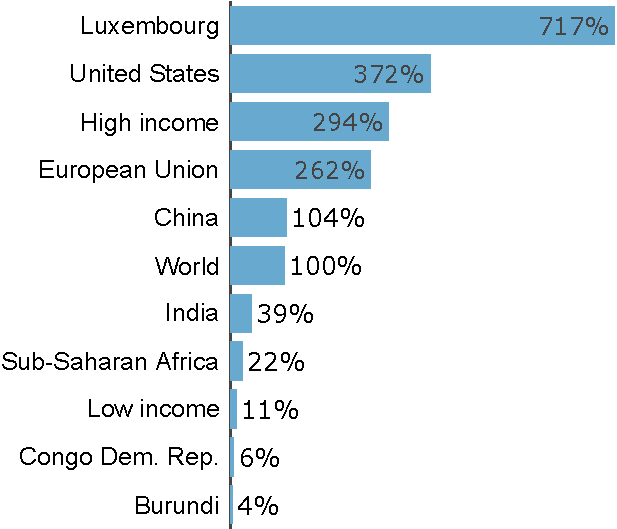
\includegraphics[width=.7\textwidth]{../figures/policies/GDP_pc_PPP.pdf}}%
\end{figure}

China's GDP per capita is now around the world average, at \euro{}1,000 per month.\footnote{Nominal GDP per capita according to \href{https://data.worldbank.org/indicator/NY.GDP.PCAP.CD?end=2022&locations=CN-1W&start=2015}{World Bank (2022)}.} %
In comparison, GDP per capita is three times higher in high-income countries and ten times lower in low-income countries (Figure \ref{fig:GDPpc}). It is hard to exaggerate the gap in living standards between countries. In fact, a transfer of just 1\% of GDP from high-income countries %
would mechanically double average income in 
low-income countries, home to 700 million people.\footnote{
Of the 26 low-income countries, defined by GDP per capita %, the following are of particular interest.
below \$1,135\/year, 22 are in sub-Saharan Africa and 4 outside (Afghanistan, North Korea, Syria and Yemen). 1.2 billion people live in a high-income country (with a GDP/capita of over \$13,845\/year).
} %

\section{The link between climate and poverty} 

Anyone who cares about the well-being of human beings wants to put an end to poverty. 
Similarly, it is not necessary to attach any intrinsic value to Nature or biodiversity in order to fight climate change; it is sufficient to be concerned about human well-being. Climate change jeopardizes the living conditions of large sections of the population, not only for future generations, but also right now, %.
particularly in tropical countries. Indeed, global warming is all the more problematic in areas that are already hot --- and home to most of the world's poor ---, as these areas are more exposed to drought, lower agricultural yields, and the difficulty of working outdoors (or without air conditioning). While the poorest are bearing the brunt of climate change, they also lack the means to cope with it: %
they don't have the resources to buy an air conditioner, build a dyke or migrate to an unscathed area. Not only does poverty increase vulnerability to climate change, climate change also increases the risk of poverty. It is estimated that between 32 and 132 million people will fall into extreme poverty by 2030 as a result of climate change (particularly through its effects on health and agricultural commodity prices).\footnote{\citet{jafino_revised_2020}.} By reducing growth in the poorest countries, climate change increases inequality: it is estimated that the income gap between the richest and poorest countries has already increased by 25\% as a result of climate change.\footnote{\cite{diffenbaugh_global_2019,khalfan_climate_2023}.} %

Climate change raises the question of the international and temporal distribution of power and wealth. %
Indeed, the distribution of greenhouse gas emissions is extremely uneven: while the richest 1\% of U.S. Americans emit an average of 318~tCO$_\text{2}$e per year, the average Indian emits 2~t and the poorest 10\% of Rwandans emit just 0.1~t.\footnote{The concept used here is the carbon footprint, i.e. the emissions attributable to individual consumption, both direct (such as gasoline consumption) and indirect (the emissions involved in producing the products consumed).} %
Globally, the top 1\% are responsible for 50\% more emissions than the bottom half of humanity.\footnote{\citet{bruckner_impacts_2022,chancel_carbon_2015}.} 
And unlike many poor Africans or South Asians who have yet to be born, wealthy, elderly Westerners with large carbon footprints are unlikely to suffer much from climate change, and therefore have little interest in changing their opulent lifestyles, unless they care about the well-being of their descendants or humans in general.\footnote{As shown by vulnerability indices \citep{chen_university_2015} or estimates of climate change damage as a function of country GDP \citep{burke_global_2015}.} 
So, to prevent the dramatic impacts of climate change, it is misleading to frame the question simply in terms of temperature, %.
because the heart of the problem lies in the inequalities between human beings who differ in terms of wealth, location or generation. As such, a solution to climate change or its impacts can only be coherent if it is equitable, and therefore involves a substantial transfer of resources from today's rich to tomorrow's poor. %


\chapter{The need for global redistribution\label{ch:redistribution_necessaire}}

\section{A moral prescription}
Whether religious, philosophical or intuitive, morality generally prescribes transfers from high-income earners to low-income earners, and therefore from high-income countries to low-income countries. This is the case with utilitarianism, the reference ethical theory used in economics. Utilitarianism attributes the same weight to each person, and thus justifies the transfer of one euro from a rich person to a poor one, since one euro will bring more satisfaction to the latter. According to the theory of optimal taxation, this reasoning is valid as long as an increase in taxes does not encourage the richest to expatriate, conceal or reduce their activity to the point of diminishing the revenues obtained. Economists have calculated the optimal tax system taking these effects into account.\footnote{In these calculations, \citet{kopczuk_limitations_2005} assume a single tax rate (a \textit{flat tax}) and do not allow for a progressive tax schedule. Without this restriction, the true optimum would be even more redistributive.} %
The theory of optimal taxation can only rationalize the current situation by turning moral on its head. Indeed, researchers have shown that the virtual absence of international transfers is only optimal if we assign a value 2,000 times higher to an U.S. American than to a Congolese (or, alternatively, if we assign a value 100 times higher to the U.S. American and consider that only one-twentieth of the money transferred will reach its recipient, the rest being diverted by corruption). %

\section{A legal-diplomatic commitment}
Beyond ethical considerations, the imperative of global redistribution has legal foundations. In 2015, all countries adopted the Sustainable Development Goals (SDGs), at the forefront of which is the elimination of extreme poverty by 2030. Yet low-income countries do not have sufficient domestic resources to eliminate extreme poverty. Indeed, in the poorest countries, expropriating all incomes from 7\textit{\texteuro} a day would not be enough to finance sufficient transfers to lift their entire population above 2\textit{\texteuro} a day by 2030.\footnote{Cf. \citet{fabre_shortfall_2024}.} %
In other words, It is impossible to achieve the first SDG without international transfers. And this, while the first SDG is limited to ensuring an income barely sufficient to avoid hunger. The transfer needed for this first SDG corresponds to 0.1\% of global GDP, or as much as is spent on pet food.\footnote{Cf. \href{https://www.grandviewresearch.com/industry-analysis/pet-food-industry}{grandviewresearch.com/industry-analysis/pet-food-industry}.} %

To ensure a decent life, which guarantees access to water, sanitation, education, a health system and a minimum ability to move about and socialize, it is estimated that an income of at least \textit{\texteuro{}}7 per day is required.\footnote{Cf. Chapter \ref{ch:premier_pas}.} 
620 million people live in a country where GDP per capita is below this threshold, and where it is therefore strictly impossible to ensure a decent life for everyone by mobilizing domestic resources alone. 
In total, half of the world's population lives below that poverty line.\footnote{Cf. \href{https://ourworldindata.org/grapher/distribution-of-population-between-different-poverty-thresholds-up-to-30-dollars}{ourworldindata.org}.} Closing the gap between their income and this threshold would cost 2\% of global GDP in 2030.\footnote{In purchasing power parity, this gap (the \textit{poverty gap}) is \textit{\$}4,800 billion, or 3.4\% of global GDP of \textit{\$}140,000 billion. Assuming annual world growth of 3.5\% (the rate observed over the last 20 years), we find a poverty gap of 
2.1\% of world GDP in 2030.} %

In 1970, industrialized countries pledged to allocate 0.7\% of their GDP to official development assistance, including 0.2\% of GDP for the least developed countries. This commitment, renewed in 2005 and 2015, has never been fulfilled.\footnote{More precisely, actual foreign aid amounts to only half of the aid promised, including only 0.06\% of GDP for the least developed countries, and only a handful of countries are meeting their commitments: Luxembourg, Sweden, Norway, Germany and Denmark. 
\citep{oecd_oda_2023}.} 
It is estimated that the bulk of the SDGs could be achieved if industrialized countries finally honored this commitment.\footnote{\citet{sdsn_sdg_2019}.} To achieve a maximalist version of the SDGs (including ensuring access to clean energy) or another ambitious target in relation to the status quo (such as ensuring \textit{\texteuro{}}7 per day for everyone), high-income countries would need to transfer more resources, probably between 2 and 5\% of their GDP.%.
% TODO %\footnote{%La \citet{cnuced_world_2023} estime à 4~\% du PIB mondial les besoins en financement pour les ODD, mais la majeure partie peut-être couverte par le secteur privé et les ressources domestiques. Une meilleure estimation repose sur 
%L'étendue de la pauvreté au seuil de 7~\textit{\texteuro{}} par jour correspondra à 4,5~\% du PIB des pays à hauts revenus en 2030, et une partie de ce coût pourrait être pris en charge domestiquement.}.% PNON unctad_world_2023


\section{An imperative for decarbonization in the South}

Lastly, a climate justice solution should be supported even by someone who would not feel bound by ethics or international commitments and would only care about the climate out of concern for her own well-being and that of her descendants. Indeed, to put an end to climate change, %--- dont les dégâts déjà supérieurs au coût de la décarbonation\footnote%{\citet{kotz_economic_2024}.} ---, TODO
the whole world needs to decarbonize. 
However, international transfers are a prerequisite for low-income countries to decarbonize. On the one hand, these countries have other priorities than decarbonization, and therefore deploy the most affordable energy system --- often based on coal. On the other hand, these countries argue --- and rightly so --- that they are the most vulnerable to climate change and have contributed only marginally to it.\footnote{Africa and South Asia combined are responsible for 6\% of cumulative CO$_\text{2}$ emissions.} 
In international negotiations, these countries generally announce two emission reduction targets: an unconditional unambitious target and an ambitious target conditional on external financing. For example, Ethiopia has pledged to unconditionally reduce its emissions by 14\% by 2030 compared with a no-climate-action scenario, and is making a 69\% reduction conditional on \$250 billion in financing. %
At the same time, developing countries (supported by the UN General Secretariat) are calling for annual transfers of \$100 billion to compensate for the loss and damage caused by emissions from developed countries.\footnote{Cf. \cite{tc_proposal_2023,sgnu_bridgetown_2023}.} While experts estimate that the transfers required would be two to four times this amount, only \$700 million were \textit{promised} in 2023 at COP 28.\footnote{Cf. \cite{songwe_climate_2023,markandya_integrated_2019,robinson_valuing_2021} and \href{https://www.theguardian.com/environment/2023/dec/06/700m-pledged-to-loss-and-damage-fund-cop28-covers-less-than-02-percent-needed}{www.theguardian.com/environment/2023/dec/06/700m-pledged-to-loss-and-damage-fund-cop28-covers-less-than-02-percent-needed}%
.}

More generally, the international arena is tending to polarize between the South, which is demanding a fairer world order, and the North, which is reluctant to give up its dominant position. For example, the African Union recently called for a global carbon pricing regime, a tax on financial transactions and a reform of the financial system, in order to benefit from dedicated, affordable and sustainable climate financing, dissociated from national and geopolitical interests.\footnote{\citet{african_union_african_2023}.} Global South countries are also critical of international negotiations on corporate taxation, which are taking place under the aegis of the OECD and exclude many low-income countries. In November 2023, although the OECD countries voted against it, the Global South countries pushed through a resolution at the UN establishing a Convention on International Tax Cooperation (akin to the climate COPs). Global South countries hope that this negotiating framework will be more favorable to their interests than the OECD. 

Despite the tendency of countries in the North to defend their short-term financial interests, there is hope that they will accede to certain demands from the South. 
Whether in defense of humanist values or to restore its often tarnished image, 
the West seeks to present itself as a model based on human rights, democracy and sustainable development. 
For example, Ursula von der Leyen, President of the European Commission, recently came out in favor of global carbon pricing,\footnote{Cf. her \href{https://twitter.com/vonderleyen/status/1700416700238225659}{Tweet} of September 9, 2023.} and a working group on international taxation (including carbon) was launched in December 2023 jointly by France, Kenya, %Spain 
and Barbados.\footnote{Cf. \href{https://www.elysee.fr/admin/upload/default/0001/15/91b013291db03bcc5f2f6b84de39a81ae0c04c7d.pdf}{https://bit.ly/taskforce\_tax}.}

Humanist values would at last be properly defended in the event of an international climate and fair taxation agreement that would make the Global North pay. Such an agreement would have the potential to rebuild geopolitics on sound foundations and pacify international relations. Conversely, it has been shown that climate change increases the risk of armed conflict, particularly in Africa.\footnote{\citet{burke_warming_2009,eberle_heat_2020}.}

In the next chapters, we propose a Global Plan to end climate change and extreme poverty, involving major North--South transfers, accepted by a majority of 
the populations of Global North countries.




\chapter{The heart of the Global Climate Plan\label{ch:coeur}}

We saw in Chapter \ref{ch:statu_quo} that there is a carbon budget that must not be exceeded to keep global warming below a given target. The Paris Agreement sets this target. Signed by all countries in 2015, it aims to contain warming ``well below 2 \textdegree{}C (...) and to pursue efforts to limit the temperature increase to 1.5 \textdegree{}C''. \\

How can we guarantee an emissions trajectory in line with this carbon budget? 

The safest approach would be to cap global emissions, with an annual cap that decreases in line with the target. \\

How then to allocate the CO$_\text{2}$ emissions allowed? 

The simplest %.
is to allocate the same emissions permit to each human. \\

Should the resale of emissions permits be authorized? 

Yes, %
Setting up a carbon market is preferable to a system of non-tradable individual carbon quotas for several reasons, detailed in the Frequently Asked Questions (FAQ, p. \pageref{q:rationing}). In particular, the market is more favorable to the poorest, as it provides financial compensation to those who do not use up all their quota.

These three answers suffice to grasp the essence of the Global Climate Plan.

\paragraph{Preventing misunderstandings}
It is important to understand that by introducing a cap on emissions, global emissions are by construction equal to this cap, thanks to mechanisms (detailed in Sections \ref{sec:pcp_quota} and \ref{sec:implementation}) that prevent it from being exceeded. This is the main advantage of this Plan.

This cap settles the temperature issue, %.
but not the social question: It is the distribution of emissions permits that determines how efforts are shared. The egalitarian distribution we propose will bring about a major North--South redistribution and put an end to extreme poverty. 

To avoid common confusion, it should be noted from the outset that this system would not allow carbon offset credits to be purchased through reforestation projects. The proposed system resembles the European carbon market in place since 2005, but is radically different from the dysfunctional and greenwashing carbon offset market.\footnote{The European market caps emissions from the industry and electricity sectors, on a trajectory that decreases to zero by 2040. It will be supplemented in 2027 by a second carbon market covering emissions from transport and buildings. These carbon markets should not be confused with the carbon offset market, which allows companies or individuals to buy carbon credits to offset their emissions through projects (such as reforestation) in developing countries. Carbon offsetting is problematic because it does not guarantee a reduction in global emissions. Indeed, it is not clear whether the projects financed result in a reduction in emissions that is \textit{permanent} (for example, an area reforested during the project may be deforested later) and \textit{additional} (for example, a forest could have grown back even in the absence of financing, or reforestation in one place may generate \textit{carbon leakage} by inducing deforestation in another). For these reasons, carbon credits are not eligible on European carbon markets. Carbon markets truly reduce European emissions.}



\paragraph{Functioning}
The system outlined above can be implemented as follows. Each year, a limited number of emissions permits are created, in line with the emissions trajectory set. These emission permits are auctioned to the companies at the source of the CO$_\text{2}$ emissions, and in particular to those who market % of their emissions.
coal, oil or gas. These companies must purchase permits corresponding to their emissions. Finally, the revenue generated by the sale of permits is redistributed as an equal basic income for all human beings. 

\paragraph{Who pays? Who receives?}
The basic income is equal to the revenue generated divided by the population. The revenue generated is equal to the carbon price multiplied by global carbon emissions. Thus, the basic income is equal to the carbon price multiplied by the average human carbon footprint. 

Although, for practical reasons, we would distribute money rather than emission permits to individuals, these two options are equivalent. Let's imagine that every human being received the same emission permit and could sell it to polluting companies on the carbon market. The amount he or she would receive would be equal to the carbon price multiplied by the individual quota, i.e. exactly the basic income. In this way, there is a perfect match between egalitarian allocation of emissions permits and egalitarian allocation of revenues. %

Even if it would be advantageous %.
to assert that the carbon price is paid by polluting companies, it is more accurate to explain that it is consumers who bear the cost. 
This is because polluting companies pass on the cost of emission permits in the form of higher prices, so that each individual faces a higher expense, equal to the carbon price multiplied by her carbon footprint. As a result, the basic income exactly covers the carbon price paid for an individual whose carbon footprint is equal to the world average. Individuals with a carbon footprint higher than the world average lose purchasing power\footnote{This result stems from assumptions justified in Appendix \ref{app:indiv}. The carbon footprint and its global average mentioned are those \textit{after} the Plan comes into force.
}. Conversely, people with a low carbon footprint gain. In other words, the proposed system operates a global redistribution from the polluters to the frugal --- so, to a first approximation, from the rich to the poor. 

To find out more, the FAQ (p. \pageref{q:riches}) contains justifications for this system compared to others, explaining how it is favorable to the poorest and would force the rich to reduce their emissions.


\paragraph{Tax or quota?}
In conclusion, this system sets a quantity: the regulator sets an emissions quota and lets the market determine the carbon price. Conversely, we could imagine a carbon tax: the regulator sets the price and lets the market determine emissions. Provided that the carbon price is the same in the system that sets the quantity and the one that sets the price, the two systems are strictly equivalent (they result in the same emissions priced at the same level). Our proposal is based on a system that fixes the quantity, since the primary objective is to respect the carbon budget (and fixing the price does not make it possible to forecast emissions accurately). The FAQ (p. \pageref{q:taxe}) explains this further. 


\paragraph{Conclusion}
To sum up, we can put an end to global warming by capping emissions, and eliminate extreme poverty with a basic income. A simple and effective system for dealing with both problems is to combine these two solutions. This is the heart of the Global Climate Plan, %.
which constitute the first two principles detailed in Chapter \ref{ch:principes}. For reasons of justice and geopolitics, a few adjustments are necessary to complete our proposal: I also describe them in Chapter \ref{ch:principes}. %
Finally, this Global Climate Plan must be complemented by other measures%.
: I outline them in Chapter \ref{ch:premier_pas}.


\chapter*{\textit{A day at Poitiers hospital}}\label{ch:narr_poitiers}
\addcontentsline{toc}{chapter}{\nameref{ch:narr_poitiers}} 

Catherine is a nurse at Poitiers Hospital. Today, she baked cakes to celebrate the end of construction work with her colleagues: now that the hospital has been renovated, there's no more drilling noise and, above all, no more unbearable temperatures during the summer months. Catherine, for her part, did not wait for the Global Plan to raise the price of gas before carrying out work on her house. When she inherited the house in 2028, the energy audit revealed that, given the anticipated price rise, the most economical option for heating was to insulate the walls and attic, and replace the oil-fired boiler with a heat pump. Repaying the works costs Catherine a little less than she would have spent on fuel oil, and by the time she finishes paying off her loan in 2041, she will really be making up for lost time. 

In her well-to-do hamlet of Charassé, almost everyone has an electric car. Catherine opted for an electric scooter when she got rid of her old Renault Twingo. She made this choice to be able to finance her daughter's business school: doing without a car saves a lot of money, especially with the rising price of petrol. And she doesn't miss the traffic jams. Even if she was apprehensive about no longer doing her shopping by car, she likes having it delivered after all. In fact, the most annoying thing is when she goes on vacation with her youngest child. Whereas it used to take her two hours to drive to her parents' home in Les Sables-d'Olonne, it now takes her six hours door to door: one bus then three trains. That's when she can't find a carpool. Thanks to the alert she's set up, she still manages to spend weekends at her parents' as regularly as before. She jumps at the chance when a driver makes a round trip similar to hers, and sometimes makes some nice encounters. Last time, she had a crush on her driver: a former worker at the closed-down aircraft engine factory, now a solar panel installer. Thinking back to his angelic smile and sun-kissed complexion, Catherine really hopes to bump into him again on the next trip.


\chapter{A widely supported Plan\label{ch:soutien}}

In addition to this book and a YouTube video\footnote{The video summarizing the book in 30 minutes is available at \href{https://bit.ly/CH_GCP}{bit.ly/CH\_GCP}.}, other volunteers and I are advocating the Global Climate Plan to multiple stakeholders through the advocacy association we founded, \textit{Global Redistribution Advocates}.\footnote{To discover all our proposals, sign our petitions, join the association or make a donation: \href{http://global-redistribution-advocates.org/}{global-redistribution-advocates.org}.} % TODO %
Our motivation to defend this Plan stems from the results of my academic research. Since my Ph.D., I have specialized in opinion surveys on climate and redistribution. I conducted an international survey in 20 countries on attitudes towards climate policies, and a complementary survey in the U.S. and Europe on opinions towards global redistribution. Although the idea at the heart of the Global Climate Plan --- a global carbon quota with egalitarian redistribution of revenues --- is long-standing and considered the canonical climate policy by economists, no survey had tested this proposal with public opinion. Surveys, however, reveal majority support worldwide. What's more, various survey methods indicate that support is sincere and could materialize electorally. 
It is this new element --- the fact that the public supports such a Plan, even in countries that would lose out financially --- that justifies putting this idea back on the international negotiating table, and giving it serious consideration. In this chapter, I will describe the history of the idea, followed by the results of opinion surveys.


\section{An old idea} 

\subsubsection{The genesis of the idea}
The polluter pays principle is a basic idea in economics, dating back to \citet{pigou_economics_1920}. The principle consists in making external costs (in this case, the damage caused by climate change) paid for by the person who causes them (in this case, the greenhouse gas emitter). This can take the form of a quota market or a tax. The cost to the polluter encourages her to reduce her activity or make it less polluting, as these alternatives are now comparatively less costly. %
Furthermore, the revenues generated by pollution pricing must be spent in the most beneficial way possible for society.  
In the case of climate change, the simplest solution is probably to share the revenues equally. This egalitarian sharing can thus be conceived as an equal emissions permit for each human. 

Given this theoretical framework, it is hardly surprising that a global carbon quota distributed on an egalitarian basis has emerged as the canonical solution to climate change ever since it first emerged into public debate. It seems that it was Michael \citet{grubb_greenhouse_1990}, a professor at University College London, who first advocated this solution when the first IPCC report was being drafted in 1990. In his article, Grubb writes that ``by far the best combination of long-term effectiveness, feasibility, equity, and simplicity, is obtained from a system based upon tradable permits for carbon emission which are allocated on an adult per capita basis.'' A year later, Anil Agarwal and Sunita Narain, of New Delhi's Centre for Science and Environment, published a seminal text on climate justice that advocated much the same solution, while castigating the ``environmental colonialism'' of developed countries. %
Since then, many have expressed their support for such a solution: \citet{bertram_tradeable_1992,baer_equity_2000,jamieson_climate_2001}, or more recently the report by \citet{blanchard_major_2021}\footnote{``The North should
frankly acknowledge its responsibility for future climate damage, and
consider the possibility of paying the South for the implementation of investments
necessary to green its economy. This could be achieved by asking the countries of the South to join a % TODO? English quote? The European Union should aim at forming a coalition of climate-ambitious countries (including the United States) with a unified ETS market. This climate coalition should encourage other countries to join its ETS in exchange for the distribution of free permits.
market mechanism and offering them free permits in proportion to their population, which would at the same time increase incentives for mitigation in developing countries.''} (former IMF Chief Economist and ``Nobel Prize'' winner, respectively) or \citet{rajan_global_2021} (former Governor of the Indian Central Bank and former IMF Chief Economist). 

\subsubsection{The failure of climate negotiations}
Alas, \citet{bertram_tradeable_1992} reports that diplomats from wealthy countries such as the U.S. and Japan evacuated this option from climate negotiations as early as 1990. At the 1992 Earth Summit, George Bush made it clear that his administration was not prepared to make any contribution to the rest of the world with his famous quote: ``the American way of life is not up for negotiation.'' %
As texts must be adopted unanimously, the UN framework has always sought a consensual solution. In the 1990s, proposals involving large-scale international transfers were rejected by countries such as the United States, while developing countries refused to accept any binding targets in the absence of such transfers. In 1997, negotiations on the Kyoto Protocol resulted in national targets for developed countries only.\footnote{\citet{gupta_history_2010}.} This division into two categories of countries turned the Kyoto Protocol into a stalemate: emissions from developing countries were not limited, while developed countries only agreed to a small reduction in their emissions (not to mention the United States, which demanded that developing countries contribute and therefore never ratified the Protocol). To break the deadlock, diplomats meeting in Copenhagen in 2009 sought to negotiate a differentiated emissions reduction for each country. Developed countries put unilateral emission reduction commitments on the table, along with a promise to contribute \$100 billion annually (one thousandth of global GDP). However, developing countries considered these commitments insufficient (the least developed countries, for example, called for a contribution of at least 1.5\% of developed countries' GDP) and refused to make binding commitments.\footnote{\citet{dimitrov_inside_2010}.} As a result, no agreement was reached in Copenhagen. Since then, ambitions have been scaled back. The Paris agreement signed in 2015 had the merit of ratifying a universal objective for limiting temperature rise, but it also formalized the transition to a non-binding regime in which each country voluntarily defines its contribution in terms of emissions reductions. 

Not only are the targets set by each country insufficient to achieve the Paris agreement objective, but the policies implemented are also likely to miss these targets. Thus, current policies and actions are taking us towards a warming of 2.6\textdegree{}C to 2.9\textdegree{}C by 2100\footnote{Cf. \href{https://climateactiontracker.org/global/temperatures/}{climateactiontracker.org/global/temperatures}.} and a temperature that would continue to rise at an alarming rate after 2100. 

In the light of the history of climate negotiations, two elements seem to be essential to obtaining a binding agreement on emissions reductions: substantial North--South transfers (of the order of 1\% of world GDP) and the abandonment of the aspiration to universality (the United States having always refused any binding agreement, to name but one).

\subsubsection{Ever-growing support from economists}
In a book entitled ``Global Carbon Pricing: The Path to Climate Cooperation''\footnote{\citet{cramton_global_2017}.}, a number of experts, including three ``Nobel Prize'' winning economists (Joseph Stiglitz, Jean Tirole and William Nordhaus), take turns extolling the merits of global pricing of CO$_\text{2}$ emissions. In this book, \citet{gollier_negotiating_2015} set out the various possible options for distributing the revenues from this pricing system according to a generosity parameter, and describe the egalitarian allocation of revenues as being the most generous towards the most disadvantaged.\footnote{The least generous allocation being that (known as \textit{grandfathering}) where revenues are allocated in proportion to emissions.} 
In another chapter, \citet{cramton_international_2015} assume that each state defends its national interest and propose the following agreement between proactive countries. %.
The generosity parameter would be chosen by countries with per capita emissions around the world average, then the climate ambition would be set at the minimum level proposed by the participating countries.\footnote{\citet{cramton_international_2015} proposes to set the price, but we could adapt their proposal to an ETS by setting the carbon budget. So I prefer to use the more general term \textit{climate ambition}.} As countries with average emissions are little affected by the international transfers implied by the agreement, they would strategically choose the parameter of generosity that would maximize climate ambition: neither too high, so that rich countries propose a high level of ambition, nor too low, so that poor countries gain and subscribe to a high level of ambition. \citet{van_den_bergh_dual-track_2020} propose a ``dual-track transition to global carbon pricing'': a \textit{climate union} that would merge existing emissions trading systems and gradually integrate new ones, and a reorientation of international negotiations (the COPs) to determine the rules of global carbon pricing and the level of generosity. The \citet{imf_how_2019} also supports global carbon pricing and, in the short term, a carbon price floor. To move towards climate justice, the institution proposes either differentiated prices between countries, or the solution we defend: a uniform price with international transfers. 

Support for global carbon pricing is not confined to \textit{mainstream} economists: it is also backed by environmental economists who favor degrowth. For example, a system equivalent to the Global Climate Plan (called \textit{cap and share} by \citealp{douthwaite_degrowth_2012}) is the first of six policy measures proposed in \textit{the economics of degrowth} by \cite{kallis_economics_2012}. Similarly, heterodox economists such as Elinor Ostrom and Robert Costanza advocate a variant of global pricing, where half of the revenues would fund a basic income and the other half low-carbon projects.\footnote{\citet{barnes_creating_2008}.}

\section{A recent discovery: public support} \label{sec:support}

In international negotiations, diplomats seem to defend short-term national interests rather than climate justice. 
But do their attitudes correctly represent the values of their peoples? 
Surprisingly, it is only recently that opinion polls have taken up the issue. All converge in finding broad support for a global, redistributive climate policy. Before presenting in detail the results of surveys carried out by my colleagues and myself examining attitudes towards the Global Climate Plan in 20 countries, %.
let's take a look at other surveys dealing with similar issues. 

\subsection{Support for global climate policies}

Over the past dozen years, a series of academic studies have focused on uncovering attitudes on the distribution of the decarbonization effort between countries. These studies cover many countries, using representative surveys of the population. While the various studies are difficult to compare, as they differ in their approach and the way they ask the questions, two regularities stand out. Whatever the country in which the survey is carried out, the preferred options are those in which the decarbonization effort is universal, and those that appear egalitarian.\footnote{For example, \citet{carlsson_is_2011} find that Swedes prefer all countries to be allowed to emit the same amount of emissions per capita. In a survey of the U.S., Germany, France and the UK, \citet{bechtel_mass_2013} reveal that a climate agreement is most preferred when it includes a large number of countries, %.
and less appreciated if rich countries are the only ones to bear the decarbonization effort compared to the option where ``rich countries pay more than poor countries'' or where countries ``pay in proportion to their emissions''. Similarly, \citet{carlsson_fair_2013} highlight that the option least appreciated by U.S. Americans or Chinese people is that where low-emission countries are exempted from any effort; while in a survey covering 28 countries (including the most populous), a large majority agree that all countries should contribute to reducing emissions \citep{dabla-norris_public_2023}. 
\citet{schleich_citizens_2016} report an identical ranking of options in China, the U.S. and Germany, with a preference for the polluter-pays principle followed by consideration of ability to pay, and last place for the option where countries that pollute the most have more rights to pollute. The authors also find that only 13 to 28\% of people (depending on the country) consider their personal position adequately represented in international negotiations; and 73 to 87\% think that the fight against climate change requires new international treaties. Finally, \citet{meilland_international_2024} find that the principle preferred by the French and the U.S. Americans is that ``all countries commit to converge to the same average of total emissions per inhabitant, compatible with a controlled climate change''.} %

Furthermore, the surveys all reveal strong support for the fight against climate change. For example, in a large-scale survey of 125 countries covering 94\% of the world's population, \citet{andre_globally_2024} find that 89\% of humans want a more ambitious climate policy, and 69\% are willing to contribute 1\% of their income to fighting climate change (a value which is a credible estimate of the cost of decarbonization). 
On the other hand, 81\% underestimate the proportion of the population willing to contribute: %.
This share is perceived on average at 43\%, 26 points lower than the reality. This underestimation (known as ``pluralistic ignorance'') of environmental concerns may explain the lack of ambition in international climate agreements. %

While most surveys investigate general or theoretical issues, very few have tested adherence to well-defined global climate measures. In fact, apart from my own studies, I know of only one, published in the scientific journal \textit{Nature}. In this five-country survey, \citet{carattini_how_2019} test different variants of a global carbon tax. For the variant with egalitarian redistribution of revenues, they find support close to 50\% in high-income countries (the U.S., Australia, UK) and South Africa, and over 80\% support in India. These results are consistent with those of the surveys I have collaborated on, detailed in \citet{fabre_international_2023} and summarized below. 

\begin{figure}[b!] %
  \caption[Support for global climate policies]{Support for global climate policies.} 
  \makebox[\textwidth][c]{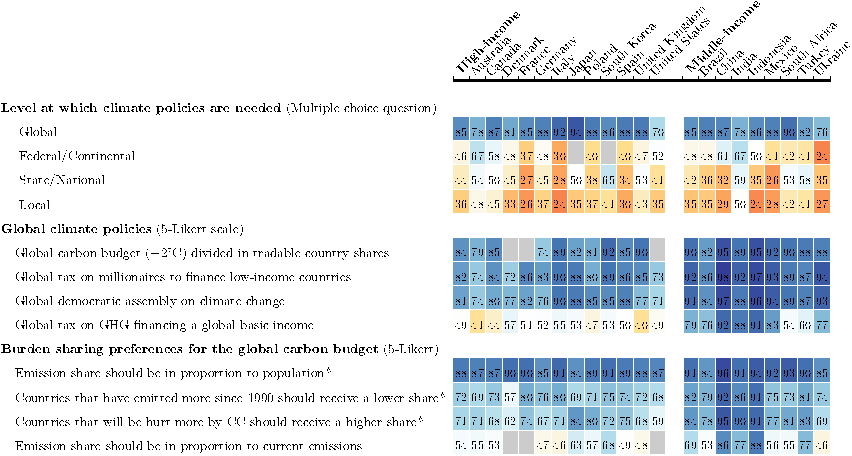
\includegraphics[width=\paperwidth]
  {../figures/OECD/Heatplot_global_tax_attitudes_share.pdf}}\label{fig:oecd} %
  {\footnotesize $\quad$ Note 1: Percentage of responses \textit{Strongly} and \textit{Somewhat support}, excluding \textit{Indifferent} responses ($n$ = 40,680). Source: \citet{fabre_international_2023}. %
  Blue denotes a relative majority. %
  \\ Note 2: *In Denmark, France and the United States, questions with an asterisk were asked differently. %
  } 
\end{figure}

The first of these surveys was carried out in 20 countries %.
between 2021 and 2022.\footnote{With my co-authors Antoine Dechezleprêtre, Tobias Kruse, Bluebery Planterose, Ana Sanchez-Chico and Stefanie Stantcheva, we conducted a survey on attitudes towards climate change and climate policies. The survey covered 20 countries accounting for 72\% of global CO$_\text{2}$ emissions (more or less the G20 countries), with representative samples of around 2,000 respondents per country. Its main aim was to study attitudes towards national climate policies, but we also asked a few questions about global measures.} It turned out that among the most supported climate measures were three global ones, each with a strong redistributive dimension: a quota of tradable emissions permits, a democratically elected world assembly that would propose a climate treaty, and a global wealth tax to fund low-income countries that meet climate targets. In every country, each of these measures receives a majority of absolute support\footnote{With one exception: the global climate assembly receives \textit{only} 48\% absolute support in the U.S.} 
and over 70\% relative support (i.e. excluding \textit{Indifferent} responses), 
as shown in Figure \ref{fig:oecd}. These results are consistent with another question which asked at what scale(s) climate policies are required: %
the overwhelming majority answered the global scale, while the continental or national scale was chosen by only a small half of respondents. 

The question on the global quota did not specify the allocation of emissions permits between countries, but the following question tested support for this measure according to different variants of permit allocation. Consistent with the preferences for the distribution of effort revealed by the above-mentioned studies, our survey uncovered a consensus in favor of allocating permits in proportion to a country's population, which corresponds to the egalitarian distribution at the heart of the Global Climate Plan.\footnote{In fact, it was precisely following this consensus that I defined the Plan on this egalitarian basis. If it were up to me, I would have preferred an even more redistributive approach than egalitarian.} This variant obtains between 84\% and 96\% relative support depending on the country, and an absolute majority of support in all countries (even including the \textit{Indifferent} responses).\footnote{The least popular variant (but still garnering a majority of relative support in most countries) allocates emissions permits in proportion to current emissions, and thus implies no North--South redistribution. An intermediate level of support (which therefore remains high) is obtained by variants that are even more redistributive than the egalitarian option: the one that takes account of historical responsibilities by allocating fewer permits to countries that have emitted more in the past, or the one that takes account of vulnerability to climate change by allocating more permits to countries that will suffer greater damage.}

Despite extremely strong support for an egalitarian global quota, a global carbon tax to fund a global basic income gets much lower support, around 50\% in high-income countries. Yet the two measures are equivalent from an economic point of view, as long as the carbon price is the same in both systems, as we saw in Chapter \ref{ch:coeur}.\footnote{Indeed, as long as the carbon price is the same in both systems, consumers face the same price increases; and the basic income distributes revenues in proportion to the countries' adult population.}  
Two factors explain this difference in support. On the one hand, people may prefer a quota to a tax, because with a quota it is certain that emissions will be reduced in line with the target. On the other hand, when asked about the carbon tax, respondents were informed of the cost of this policy on their purchasing power. Without a complementary survey, we could not know the level of support for the Global Climate Plan (i.e. the equal quota) when people are informed of the loss of purchasing power it would entail.\footnote{The amounts of these losses are reported in notes \ref{fn15}-\ref{fn16} and the method of calculation in Appendix \ref{app:pays}.}   


\subsection{Strong support for the Global Climate Plan}

To gain a deeper understanding of attitudes towards the Global Climate Plan, in 2023 I conducted a complementary survey with two new co-authors: Thomas Douenne and Linus Mattauch. This survey is based on a representative sample of 3,000 Europeans (in Germany, Spain, France and the UK) and two representative samples of (respectively) 3,000 and 2,000 U.S. Americans. 

Even with a clear understanding of the loss of purchasing power involved, 76\% of Europeans and 54\% of U.S. Americans support the Global Climate Plan (see Figure \ref{fig:gcs_support}).\footnote{\label{fn15}
Here is how we described the measurement to respondents:
\begin{quote}
At the Paris agreement in 2015, all countries have agreed to contain global warming ``well below +2 $\mathrm{{}^\circ}$C''. To limit global warming to this level,~\textbf{there is a maximum amount of greenhouse gases we can emit globally}.\\
To meet the climate target, a limited number of permits to emit greenhouse gases can be created globally. Polluting firms would be required to buy permits to cover their emissions. Such a policy would~\textbf{make fossil fuel companies pay}~for their emissions and progressively raise the price of fossil fuels.~\textbf{Higher prices would encourage people and companies to use less fossil fuels, reducing greenhouse gas emissions.}\\
In accordance with the principle that each human has an equal right to pollute, the revenues generated by the sale of permits could finance a global basic income.~\textbf{Each adult in the world would receive } \textbf{\euro{}30/month}, thereby lifting out of extreme poverty the 700 million people who earn less than \$2/day.\\
\textbf{The typical }[\textbf{German}]\textbf{ would lose out financially }[\textbf{\euro{}25}]\textbf{ per month}\footnotemark{\label{fn16}} (as he or she would face [\euro{}55] per month in price increases, which is higher than the [\euro{}30] they would receive). 
\\The policy could be put in place as soon as countries totaling more than 60\% of global emissions agree on it. Countries that would refuse to take part in the policy could face sanctions (like tariffs) from the rest of the World and would be excluded from the basic income.
\end{quote}
We then made sure that respondents had understood who would gain or lose from this measure, and in particular that it would be costly for typical people in their country. To do this, we asked comprehension questions, then displayed the correct answer. Finally, we described the measure again, more succinctly, before testing support with a Yes/No question.} 
\footnotetext{\label{fn16}This median net monthly cost is adjusted by country. It is \$85 in the United States, \euro{}10 in France, \euro{}5 in Spain and £20 in the United Kingdom.} 
In Europe, whatever the country or political position, a large majority supports the Global Climate Plan. 
In the United States, there is a strong polarization: 74\% of Biden voters support the Plan while 74\% of Trump voters oppose it, with abstainers supporting it at 53\%.  
These results show that most Westerners are willing to lose a few dozen euros a month if it will put an end to climate change and extreme poverty.\footnote{Support is greater for the quota than for a carbon tax (tested in the 20-country survey), confirming that the population prefers a measure that they are certain will sufficiently reduce CO$_\text{2}$ emissions.}

\begin{figure}[h!]
  \caption[Support for the Global Climate Plan]{Support for the Global Climate Plan (percentage of \textit{Yes}).} 
  \makebox[\textwidth][c]{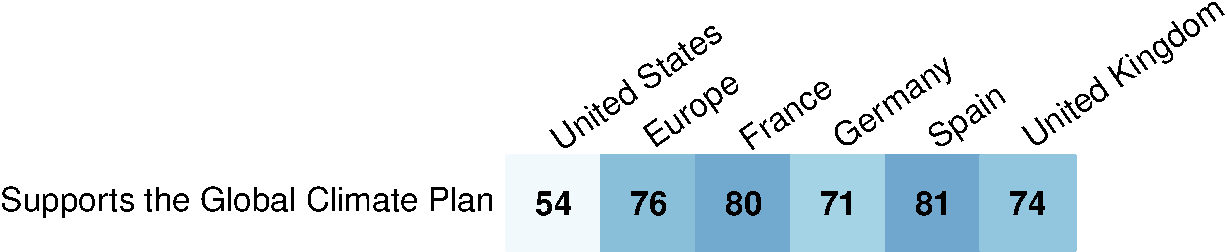
\includegraphics[width=\textwidth]
  {../figures/country_comparison/gcs_support_positive.pdf}}\label{fig:gcs_support} 
\end{figure}

\subsection{Genuine support} %

Despite the very favorable responses to the Plan, one might question the declared support. 
The only way to be absolutely certain that a majority of the population sincerely supports the Plan would be to organize a referendum. That said, even a simple survey can give a good indication of the sincerity of responses, and we used a number of methods to test this sincerity in the remainder of the survey.

To get as close as possible to the stakes involved in a referendum, we asked respondents whether they would be prepared to sign a petition in support of the Global Climate Plan, in the knowledge that the results of this question (asked to a representative sample of the population) would be forwarded to the Head of State's office. In this way, respondents understood that their response could influence official policy. In the U.S., a majority is prepared to sign the petition, and the difference with direct declared support is not significant. In Europe, 69\% of respondents are prepared to sign the petition: this is 7 points less than for declared support, but still a large majority. 

Using a technique called ``list experiment'', we show that support is genuine and not driven by a possible social desirability bias. This experiment works as follows: we ask respondents \textit{how many} measures they support from a list of measures, and so we don't know which measure a respondent supports.\footnote{As a result, respondents no longer face a social desirability bias prompting them to lie about their support for this or that measure.} 
For a random half of the respondents, we add the Global Climate Plan to the list of measures.\footnote{In Europe, the three other measures on the lists are: the death penalty for major crimes, a national redistribution plan and a building insulation plan.} 
By calculating the difference between the average number of measures supported in the groups with and without the Plan in their list, we can estimate the tacit support for the Plan.\footnote{For example, if the \textit{group without} the Plan supports an average of 2.1 measures, and the \textit{group with} the Plan supports 2.86 measures, we can assume that the \textit{group with} the Plan supports the other measures as much as the \textit{group without} (since they are each representative of the population), and that the difference between the number of measures supported corresponds to support for the Plan, i.e. $2.86 - 2.1 = 76\%$ tacit support for the Global Climate Plan.} %
Tacit support is not significantly different from declared support, indicating that respondents are not pretending to support the Plan in order to satisfy a social norm.\footnote{In other contexts, this method has revealed a social desirability bias in favor of the invasion of Ukraine among the Russian population (tacit support being 10 to 20 points lower than declared support), or the under-reporting of racist opinions in Southern U.S. \citep{kuklinski_racial_1997,chapkovski_solid_2022}.} 

\subsection{An electoral gain from campaigning for the Plan}
The most convincing proof that support for the Plan runs deep is that a progressive candidate could win votes by supporting it. We show this through a number of questions. First, we describe a progressive and a conservative program corresponding to the typical programs of the main parties in the country.\footnote{We present the choice between the two programs as that between the two candidates in the next major election, % [country]
and then ask respondents which candidate they would vote for.} For a random half of the sample, we add the Global Climate Plan to the progressive program. In France, the progressive candidate would gain 11 points in vote intentions by including the Plan in her or his program. In the U.S., the progressive candidate could gain 3 points, while in the other countries, the effect is not statistically different from zero.\footnote{The electoral gain is highly significant in France (the $p$ value is 0.5\%). For the U.S., the $p$ value is 13\%, i.e. not statistically significant at the usual 5\% threshold, but with only a 13\% chance that the progressive candidate would have no electoral gain by supporting the Plan. For the other countries, the electoral gain is not significantly different from zero (even at the 20\% threshold).} 
Thus, support for the Global Climate Plan would not cost a progressive candidate votes in any country, and could yield a significant electoral gain in France. 

In the next question, we draw two political programs from a set of (rather progressive) measures, then add the Plan to one of the programs.\footnote{In Europe, respondents are asked to imagine that a left- or center-left coalition will win the next election, and are asked on which program they would prefer this coalition to have been elected. In the U.S., the question is framed as a hypothetical duel in a Democratic primary and asked only to non-Republicans (i.e. Democrats, independents and non-affiliated).} The program containing the Plan is systematically preferred by a majority (ranging from 58\% in the U.S. and UK to 64\% in Spain, cf. Figure \ref{fig:conjoint_left_ag_b}). This question and the previous one reveal that support for the Global Climate Plan is not only sincere, but is also important enough to determine the electoral choice of some voters.\footnote{This interest in 
global redistribution is confirmed in a question asking respondents to allocate 100 points to express their support for a set of measures (the same as above), with the instruction to award more points to the measures they support most. The Global Climate Plan is given higher than average priority, and is one of the most popular climate policies. Conversely, a climate measure enacted in the EU and California (the phase-out of new internal combustion cars) is one of the three least prioritized measures in each country. More generally, this question shows that global redistribution measures are a fairly high priority for the electorate, just behind the most popular measures: raising the minimum wage and improving public services through additional funding for education and healthcare.} 

\begin{figure}[h!] 
  \caption[Influence of Plan on preferred program]{Influence of the Plan on preferred program:\ Preference for random program A containing the Global Climate Plan over program B not containing it (in \%). (In the U.S., question asked only to non-Republicans).}\label{fig:conjoint_left_ag_b}
  \makebox[\textwidth][c]{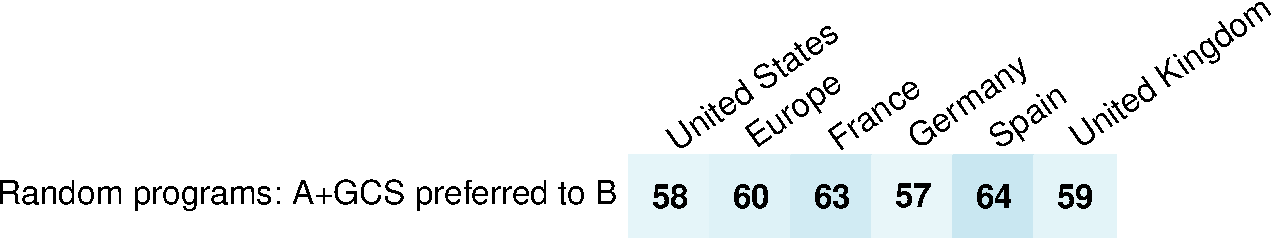
\includegraphics[width=\textwidth]{../figures/country_comparison/conjoint_left_ag_b_binary_positive.pdf}} 
\end{figure}


To sum up, the opinion polls reveal broad and sincere majority support for the Global Climate Plan, and indicate that the population prefers political programs that include this measure to those that do not. And this despite the fact that Western respondents are fully aware that they would lose some purchasing power under the Global Climate Plan. 

If people support this Plan, it is because it is fair and global, and therefore effective in putting an end to climate change. This was not the case with the French carbon tax, which the Gilets jaunes opposed, and whose rejection was clearly measured in opinion polls. In other words, most people are concerned about the climate, and willing to support a solution as long as it is fair and effective. 
To find out more about these surveys, I refer the reader to the academic article entitled \href{https://papers.ssrn.com/sol3/papers.cfm?abstract_id=4448523}{\textit{International Attitudes Toward Global Policies}}, which I co-authored with Thomas Douenne and Linus Mattauch. 

\chapter*{\textit{Unfolding the dream political future}}\label{ch:narr_reve}
\addcontentsline{toc}{chapter}{\nameref{ch:narr_reve}} 

The year I was born, the first conference on climate change was held. It was 1992, and economists were already dreaming up what would later become the Global Climate Plan. This idea was swept aside by the United States during the negotiation of the Kyoto Protocol, but received renewed interest when a study financed by the OECD revealed in 2023 that almost 80\% of the population would support this Plan in all countries. This marked the start of a marathon of advocacy, first with economists, easy to convince, then with associations, less responsive, and finally to the political world. At the time of writing, the Plan has already received the blessing of several ``Nobel Prize'' winners, and we have presented it to the Chinese, Indian, Brazilian, French, German, Spanish and South African governments, all of whom have been receptive. Seventeen candidate lists have officially endorsed it to the European election representing 64 Members of the European Parliament from ten different countries and four political groups (Renew, S\&D, The Greens, The Left). %(including Ecologistes -- EELV, Parti Socialiste and Renaissance -- Besoin d'Europe in France, and Sumar in Spain). TODO [country]
This is the history we can write together, to put an end to climate change and extreme poverty: 

~[\textit{Beginning of fiction}] The Brazilian presidency of COP30 put forward the idea ahead of the 2025 summit. It is immediately supported by Greta Thunberg and UN Secretary-General Antonio Guterres. 
Behind the scenes, the Chinese Foreign Minister is discussing the Plan with his European counterpart.  
Even if the negotiations remain secret, the German Social Democrats and Greens have decided to campaign on this Plan in the 2025 elections. 
Against all the odds, their coalition wins by a landslide. 
All hell breaks loose. In November 2025, Brazil, the European Union, China and India make this plan their common position at COP30. Following Donald Trump's re-election, the United States obviously rejects the agreement, but the governors of California and New York state make it known that their states will join the agreement, even if the federal level does not follow suit. African countries can't believe their eyes: 
are we really going to get an international agreement %?
on a plan that would double the average income of a country like Burundi, by paying every human a basic income of \euro{}50/month? In February 2026, a group of 156 countries and 9 U.S. states, covering 74\% of global CO$_\text{2}$ emissions, sign an agreement in principle to negotiate a cap on their CO$_\text{2}$ emissions. What follows is a five-year battle to negotiate the plan, followed by a painstaking implementation, which is delayed but fully operational by 2037. Boosted by the basic income, Africa experiences an unprecedented economic boom. In the 2050s, the U.S. and Russia finally join the Climate Union. Saudi Arabia is the last country to take the plunge, in 2061. By 2084, the entire world has achieved carbon neutrality, and no one lives on less than \textit{\texteuro{}}7 a day. It is not a foregone conclusion: half of humanity is living below this poverty line at the time of writing. %
And you, strikers --- I am sure you're part of it ---, you've got a lot to do with it. Indeed, none of this would have been possible without the global strike for justice and climate in October 2025, followed by almost a billion people.

\chapter{The main elements of the Global Climate Plan\label{ch:principes}}

The proposal developed in this chapter does not solve all humanity's problems, nor is it a complete answer to climate change. Although it is referred to as the ``Global Climate Plan'' (because it is more punchy), ``International Framework for the Phase Out of Fossil Fuels'' would have been more accurate.  %
As it stands, the Plan only covers fossil and industrial CO$_\text{2}$ emissions, not those linked to land use, forestry or other greenhouse gases. %
Its scope is limited to establishing a framework treaty that guarantees emissions reductions and determines international transfers. It is then up to each State or local authority to take the appropriate (climate and social) policies to ensure that decarbonization proceeds smoothly on its territory. Now that the scope of the treaty has been defined, % of
let's take a look at the Plan's main principles.

\section{1$^\text{st}$ principle: An annual emissions quota}\label{sec:pcp_quota}

The carbon budget --- and with it the future climate --- is the decisive element that the States will have to negotiate. 
Our proposal is based on a net emissions budget and covers the period when net emissions are positive, i.e. when emissions exceed sequestration (see below). Figure \ref{fig:emissions_par_region} illustrates a global emissions trajectory on which countries could agree, and projects the trajectories it might imply in different regions (see details in Appendix \ref{app:pays}). 

\begin{figure}[h!]
  \caption[Emissions trajectories by region]{Estimated trajectories of CO$_\text{2}$ emissions per adult in different regions for a +1.8\textdegree{}C scenario}\label{fig:emissions_par_region}
  \makebox[\textwidth][c]{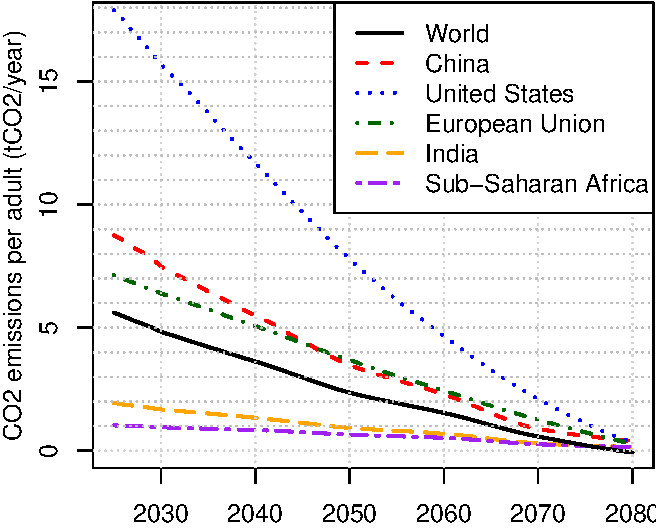
\includegraphics[width=.92\textwidth]{../figures/policies/emissions_per_region_sm.pdf}} %
\end{figure}



The carbon market works as follows. 
The Plan's governing body defines the annual emissions quota, in line with the carbon budget. At the beginning of the year, this quota is auctioned. %
Regulated companies are those that market hydrocarbons (coal, oil, gas) or whose industrial processes emit CO$_\text{2}$ (cement production, hydrocarbons, incinerators). 
Each regulated company announces the quantity of permits it is committed to purchasing at each carbon price level. For each possible price, we thus obtain an aggregate quantity requested by the regulated companies, which decreases with the price. Emission permits are then sold at the price for which the aggregate quantity requested corresponds to the quota. Regulated companies and approved financial institutions can then trade emissions permits on a secondary market. After a few years (possibly one or two), 
the equilibrium price will have been discovered, so that the price on the secondary market will be relatively predictable and equal to the auction price. At the end of the year, emissions from regulated companies are monitored, and these companies are required to deliver permits covering their emissions. %
Deterrent penalties ensure that the system works properly. For example, for every tonne of CO$_\text{2}$ emitted but not covered by an emissions permit, the offending company must pay a fine equal to three times the price of a tonne of CO$_\text{2}$, and must still deliver the missing permit the following year. In addition, a country risks exclusion from the system if it fails to apply the Plan correctly on its territory. %

In short, an emissions trading system (ETS) would be set up to cap CO$_\text{2}$ emissions on an international scale. 
Such a system has already proved its worth in several countries, including the European Union,\footnote{The European ETS is often criticized. However, it has in fact enabled covered emissions (from industry and power generation) to be reduced in line with the target, while uncovered emissions (which will be covered from 2027) have continued to rise. In reality, the European ETS has been criticized for two (good) reasons. Firstly, the target set was not ambitious enough (which explains the very low price until a reform of the system in 2019). Secondly, emission permits were allocated free of charge to polluting companies, rather than being auctioned. The Global Climate Plan avoids these two pitfalls.} 
China and South Korea, and is under consideration in others such as India, Brazil and Nigeria. 17\% of global emissions are already covered by an ETS. What's more, different ETSs can be successfully merged, as California and Quebec have shown.\footnote{\citet{icap_emissions_2023}.} In the case of the proposed Plan, the new ETS would be added to existing ETSs rather than merged with them, to avoid reducing the ambition of any of them. In particular, the European ETS has a rapid decarbonization trajectory, since from 2040 no more emission permits will be created for electricity and large industrial plants.\footnote{\citet{pahle_emerging_2023}.} Incidentally, the ongoing decarbonization of the EU shows that the carbon market is working as intended.

\paragraph{Negative emissions}
There are several ways of sequestering carbon from the atmosphere, including reforestation (and, more generally, biomass gains), bioenergy with carbon capture and storage\footnote{BECCS involves growing plants, incinerating them (which, incidentally, provides energy), recovering most of the CO$_\text{2}$ from the plant's chimneys, and then sequestering this CO$_\text{2}$ in underground cavities.}, or direct capture of CO$_\text{2}$ from the air.\footnote{Direct Air Capture technologies extract CO$_\text{2}$ from the air using a liquid solvent or a solid absorbent.} 
To reach the 1.5\textdegree{}C target by 2100, such negative emissions will be necessary, especially at the end of the century, when more affordable decarbonization actions will have been carried out.\footnote{\citet{minx_negative_2018}.} 

In this book, we interpret the Paris Agreement as allowing for a temporary overshoot of the 1.5\textdegree{}C target, provided that warming does not exceed 2\textdegree{}C. In other words, net negative emissions (from the second half of this century onwards) will make it possible to get back down to 1.5\textdegree{}C, a threshold that will very likely already be crossed in 2040.\footnote{\citet{diffenbaugh_data-driven_2023} estimate that warming will exceed 1.5\textdegree{}C in 2035 in an ambitious decarbonization scenario, which is consistent with Table 4.2 of the \citet{ipcc_climate_2021} report.} 
To fix ideas, say that the positive emissions budget would be 1,000 GtCO$_\text{2}$ from 2025. This carbon budget is in line with the objective of not exceeding 2\textdegree{}C of warming.\footnote{More precisely, there is a two-in-three chance of not exceeding 2\textdegree{}C of warming with a carbon budget of 1,000 GtCO$_\text{2}$ from 2024.} % TODO! update figure to 2025
In the next phase, where net emissions will be negative, there would be two annual carbon budgets: a quota of residual positive emissions (for activities that are impossible to decarbonize), and a tender for negative emissions. An annual call for tenders would enable these negative emissions to be purchased at the lowest cost, and this carbon sequestration would be financed by taxes on the wealthiest, such as a global wealth tax.\footnote{Only projects whose sequestration is indisputable would be financed. For example, sequestration through gains in forest biomass would only be financed if the emissions linked to the loss of forest were also priced. Carbon sequestration could also be financed from the very first phase, again through taxes on the wealthiest. Its value would then be set at the market carbon price, and the sequestration thus remunerated would swell the auctioned emissions quota by the same amount \citep{edenhofer_governance_2023}.} %
After a few decades of net negative emissions, we would reach the Paris Agreement climate target (1.5\textdegree{}C warming), and we could even continue to sequester carbon to achieve a milder climate and limit sea-level rise. In this book, we do not concern ourselves with negative emissions, which will only become significant in a few decades' time, and focus on the first phase of the Plan. 

\section{2$^\text{nd}$ principle: A global basic income}\label{pcp:rdb}

\begin{figure}[bh!]
  \caption[Trajectories (emissions, price, basic income)]{Estimated trajectories of emissions, carbon price and basic income}.\label{fig:trajectory}
  \makebox[\textwidth][c]{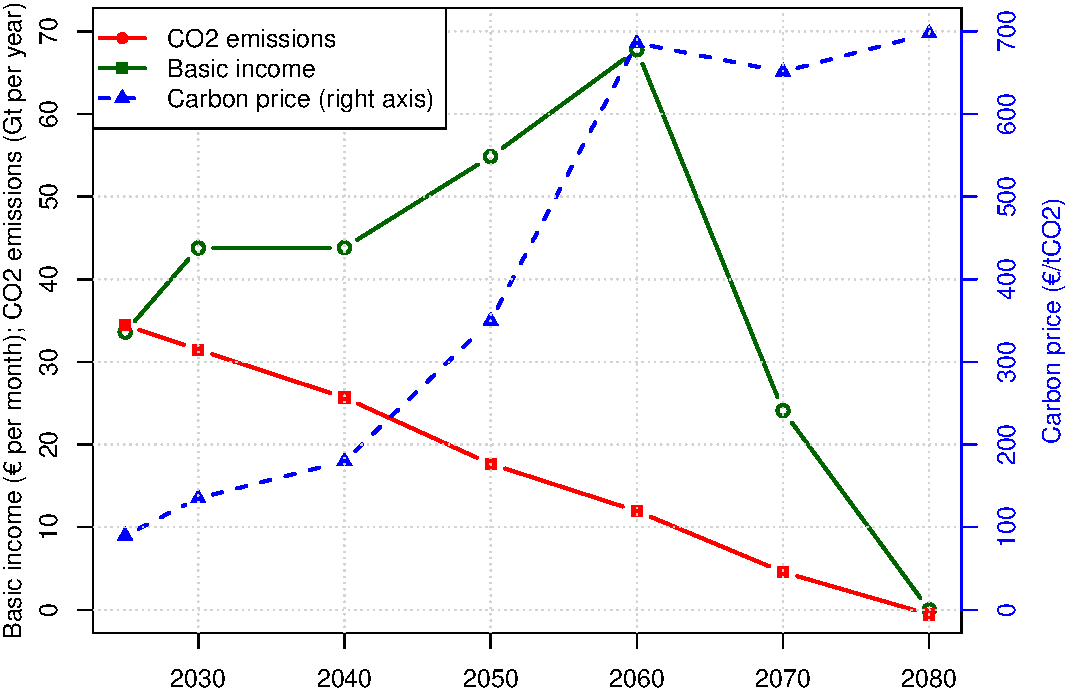
\includegraphics[width=\textwidth]{../figures/policies/GCP_trajectories.pdf}} 
\end{figure} 

The Plan's revenues would be used to finance a global basic income: the same transfer to all humans aged 15 or over.\footnote{In reality, it would be better to also pay a basic income to (parents of) children under 15, of an amount less --- say half --- than that received by adults. This book models the no-basic-income-for-children option to keep in step with the question posed in the survey.
} 
We estimate that the basic income would amount to \euro{}44 per month in the first few years\footnote{The basic income is estimated by multiplying the carbon price by global emissions and dividing by the world's adult population. Those paying close attention will note that this amount is higher than that used in the survey (\euro{}30 in 2030, cf. \citealp{fabre_global_2023}). Indeed, for this book, I have redone the calculations using a more sophisticated model (cf. Appendix \ref{app:pays}), and the resulting carbon price is higher than that of my initial source \citep{stern_report_2017}.} (from 2030 to 2040), which would be enough to lift the 700 million people living on less than \textit{\texteuro{}}2 a day out of extreme poverty. 
The basic income would then increase slightly, reaching an average of around \euro{}50 per month between 2030 and 2060 (see Figure \ref{fig:trajectory}), before declining rapidly as the world approaches zero net emissions (a milestone reached in 2079 in our scenario). 
At its peak in 2030, the Plan's revenues are estimated at 2.5\% of global GDP. The Plan would generate international transfers of around 0.6\% %.
of the world's GDP, the remainder %.
of revenues being repaid inside the country in which they are collected. 
The Plan's distributive effects per person and per country are detailed in Chapter \ref{ch:effets_distributifs}. 
For example, the average European % [country] 
would lose 25\euro{} per month as a result of the Plan in 2030, while the average Indian would gain 25\euro{} per month. %

Compared with alternative uses of revenue, the basic income has the advantage of reaching the poorest and leaving no one behind. What's more, it is adapted to the varied situations of individuals, who decide for themselves how to use the money according to their needs (food, care, equipment, etc.). 
Although distributing a basic income to every person is technically difficult, various options are available %.
(see section \ref{sec:implementation}). If the infrastructure is not ready in time for distribution, or if communities prefer to receive the money in another form, the money could be paid to local or national authorities to develop public services, social protection and infrastructure (see FAQ, p. \pageref{q:rdb}). 

\section{3$^\text{rd}$ principle: A climate union}

The Plan would be launched by a union\footnote{Economists call it a \textit{climate club}.} of voluntary countries and implemented as soon as 60\% of global CO$_\text{2}$ emissions are covered by the participating entities.\footnote{Note that sub-national entities could join the union even if the federal level does not.} This threshold could be reached by the union of China (30\% of global emissions), the U.S. (15\%), India (7\%), the EU and the UK (9\%). If the United States does not participate, this threshold would still be reached in a \textit{prudent} scenario where the union would be formed by the EU, the countries that would benefit financially from the Plan (19\%, including India) and those that would neither gain nor lose financially (36\%, including China).\footnote{The notion of gain or loss refers to the monetary flows of the carbon market and the basic income, and is understood in relation to a situation with the same emissions reductions but without international transfers (cf. Chapter \ref{ch:effets_distributifs} and Appendix \ref{ch:methodo}).} %
In an \textit{optimistic} scenario, where we add to this the other states likely to join the union,%, we will be able to say that we're in the midst of a major change.
\footnote{In addition to the countries that would not lose out financially and the EU, we can expect participation from the following states: Japan, South Korea, Canada, the UK, Norway, Switzerland, New Zealand, as well as the 12 U.S. states where the Democratic Party won the last election by more than 15 points (in particular the West Coast, Illinois and the Northeast with the exception of Pennsylvania).} 
91\% of the population and 74\% of global emissions would be covered (see Table \ref{tab:scenarios_table}). 

\begin{table}[h]

\caption{\label{tab:scenarios_table.tex}Main features of the different scenarios.}
\centering
\begin{tabular}[t]{ccccc}
\toprule
Scenario & \makecell{Emissions\\covered} & \makecell{Population\\covered} & \makecell{Basic income\\in 2040 (\$/month)} & \makecell{EU loss in 2040\\(share of its GDP)}\\
\midrule
All countries & 100\% & 100\% & 47 & 0.8\%\\
All but OPEC & 90\% & 97\% & 41 & 0.9\%\\
Optimistic & 74\% & 93\% & 32 & 1.1\%\\
Central & 67\% & 90\% & 25 & 1.1\%\\
Prudent & 63\% & 88\% & 22 & 1.2\%\\
Africa EU & 12\% & 24\% & 29 & 1.1\%\\
\bottomrule
\end{tabular}
\end{table} 

To prevent the displacement of emissions to countries with less restrictive legislation, imports into the Union would be taxed in proportion to their carbon content: this is the carbon tariff. It is compatible with WTO rules, and the EU is implementing it at its borders.

A climate union would strengthen the Paris Agreement, by operationalizing its Article 6. This article enables states to set up a carbon market, but can only become operational if countries agree on a precise carbon budget and its allocation. The union of a majority of countries could unblock the situation, as long as these countries adopt a common standard to define their Nationally Determined Contribution (using the one implied by the Plan, based on the same carbon budget for each person). This union would thereby accept North--South redistribution and acknowledge the lack of solidarity of recalcitrant countries. 

A universal climate union would make it possible to respect the carbon budget mentioned above, and thus limit the rise in global temperature to 1.8\textdegree{}C, compared with a rise of 2.7\textdegree{}C in the absence of additional measures. In the \textit{central} scenario, where participating countries account for only two-thirds of global emissions, the temperature rise would still be contained at 2\textdegree{}C in 2100.\footnote{The emissions of participating countries are assumed to follow the IPCC RCP-2.6 scenario, and those of non-participating countries the RCP-4.5 scenario, whose temperature rise in 2100 closely matches that projected on the basis of current measurements, according to the IPCC (AR6, WGI, Chapter 1).}

\section{4$^\text{th}$ principle: Participation mechanisms}

Without additional adjustments, the Plan would have the effect of making countries with carbon footprints above the global average net contributors, including some countries whose populations are far from wealthy. To take account of the limited ability of these populations to pay, a \textit{waiver} would prevent countries with intermediate incomes from being net contributors. Such derogatory clause would allow countries whose per capita GDP does not exceed the world average by more than 50\% (such as China, South Africa or Algeria) to keep the revenues collected on their territory. These countries would face the same decarbonization constraints as the others, but would neither win nor lose compared to a carbon pricing system without international transfers. 

The treaty would also allow individual % SJ added 'individual' 
states, % SJ added comma
such as California and New York, % SJ added comma
to join the union independently of the federal level. In particular, these states would be exempt from carbon tariffs, % SJ added 's'
as they cannot impose a tariff on other U.S. states. 
These mechanisms are detailed in Appendix \ref{ch:details}. 


\section{Implementation}\label{sec:implementation}
In addition to the geopolitical challenge, the implementation of the Plan would face two technical challenges. 

\paragraph{Emissions monitoring, reporting, and verification}

The first challenge is that carbon emissions must be reported, monitored and verified, at least % of the time. % SJ is this missing a number? => no
for large industrial units such as coal mines or oil refineries. This could prove difficult in countries without % SJ removed 'an'
efficient administration. However, this challenge is not specific to the Plan, as emissions control is a necessary element of any successful climate policy. In fact, emissions control is likely to be made easier by the Plan than by other climate policies, since the Plan would provide resources to low-income countries which they could use to develop their administration % SJ removed brackets from 'which- administration
and make % SJ 'enable countries to'
countries work together. % SJ added full stop
% SJ added 'in this way, more' 
In this way, more experienced countries would help others. In addition, U.S. and European projects now make it possible to use satellites to measure the emissions of an industrial facility, a locality or a country.\footnote{\citet{pan_potential_2021,shen_national_2023} and the \href{https://www.esa.int/Applications/Observing_the_Earth/Copernicus/Carbon_dioxide_monitoring_satellite_given_the_shakes}{ESA CO2M project}.} These measurements are used to check the reliability of reported emissions.

\paragraph{Distributing basic income} % SJ I think to be consistent, make these headers.
Secondly, the basic income must be accessible to everyone, % SJ changed 'all' to 'everyone' + added comma
and fraud-resistant, % SJ added comma
so that no one % SJ removed hyphen
receives the basic income more than once. % SJ brackets removed from 'so - once'
It is difficult to reach people who have no civil status or who live in remote areas. Similarly, it is difficult to verify people's identities and make sure they aren't registered more than once. However, there are good reasons to be confident that the infrastructure needed to provide % SJ deliver -> provide
a basic income can be deployed within ten years, as various technical solutions are available. Firstly, most countries already have social programs for isolated people % SJ removed commma
and are carrying out population registration campaigns, including electoral registers. %
Secondly, smartphones can now be used as a means of payment and for biometric identification (and the cost of a smartphone would be covered by just a few months' basic income). %
Thirdly, %.
Satellite Internet offers an affordable solution for accessing the Internet from anywhere. In practice, the basic income of the inhabitants of a small village would be more than enough to cover the Starlink subscription (\euro{}17 per month in Nigeria) as well as the equipment (\euro{}190).\footnote{Cf. \href{https://starlinkinsider.com/starlink-price/}{starlinkinsider.com/starlink-price}.} %


\paragraph{Advanced identification}
Progress in these infrastructures has been meteoric. Launched in 2009, India's Aadhaar system has provided a unique biometric identifier for 99\% of the adult population in just 8 years\footnote{Cf. \href{https://www.thehindu.com/business/Aadhaar-covers-99-of-adults-in-India-Prasad/article17104609.ece}{thehindu.com}. 
A number of problems have marred Aadhaar in the past, but % SJ (we can learn from these failures to avoid repeating them. What works is now better known.) This can be replaced by 'lessons have been learned.' 'learnt' - UK English.
For example, the best practice is to use open-source protocols for biometric identification (\href{https://mosip.io}{MOSIP}) rather than proprietary software.} at a cost of just 1\euro{} per registered person. This deployment of biometric identity is now being replicated elsewhere. %
In particular, the World Bank's \textit{Identification for Development} program finances identification systems in % SJ (57)
fifty seven of the world's poorest countries,\footnote{Cf. \cite{world_bank_state_2017,world_bank_benin_2020,world_bank_identification_2022}.} with the aim of % AF " => ``
``providing legal identity for all'' in line with Sustainable Development Goal n\textdegree{}16.9. This identification then makes it possible to offer numerous services % SJ removed comma
and could be used for % SJ removed 'the'
basic income. 

In India, Aadhaar is linked to bank accounts and is % SJ -> added 'is'
already used to distribute social benefits. In less than two weeks, Togo has set up a mobile money transfer for one million people to compensate for the loss of income suffered by informal workers in confined areas during the COVID pandemic.\footnote{\citet{ipa_togos_2021}.} 

Although the technical challenge remains, it seems to be one that can be met by an appropriate combination of existing and new infrastructure, tailored to the specific needs of each region. 

\paragraph{Haiti as first test}
A country like Haiti could be a test case for the successful implementation of a basic income. Taking a small island as a first test would avoid the movement of people from neighboring % SJ 'neighbouring' UK
countries to receive the basic income. % SJ not a \footnote{
The average income in the Dominican Republic is seven times higher than in Haiti, allaying fears of an influx from this single-border % SJ -> added hypen
country. % SJ } 
What's more, Haiti is not only one of the poorest countries in the world, but also one where the administration is failing and overtaken by armed gangs. If the distribution of a basic income is successful even in such a situation, it is reasonable to assume that it can be implemented anywhere. % SJ generalized -> implemented anywhere
Furthermore,% SJ Moreover -> Futhermore
distributing a basic income of 44\euro{} per month to all Haitian adults for four years would cost 17 billion euros, a sum that could be financed by a single state, % SJ -> comma 
or even by a private consortium % SJ (or even by a private consortium) -> or even by a private consortium. %
For example, the French state could provide this financing and thus repay the illegitimate debt that France imposed on Haiti at the time of its independence;
a debt imposed to compensate its slave-owning colonists. % SJ (a debt imposed to compensate its slave-owning colonists) -> a debt imposed to compensate its slave-owning colonists.
\footnote{Cf. \href{http://preferences-pol.fr/Documents/Haïti.pdf}{preferences-pol.fr/Documents/Haiti.pdf}.}%.


\chapter{A major transfer to the Global South\label{ch:effets_distributifs}}

As we saw in Chapter \ref{ch:coeur}, the Global Climate Plan would redistribute resources from people with a higher carbon footprint than the global average to those with a lower carbon footprint. In this chapter, I present estimates of the Plan's effects on the global distribution of living standards, the share of people gaining financially from the Plan in each country, and maps of gains and losses by country. The methodologies used % SJ employed -> used
are explained in Appendix \ref{ch:methodo}.

\section{The end of extreme poverty}\label{sec:fin_pauvrete}

Seventy-one percent % SJ 71% -> seventy-one percent
of humans would benefit financially from the Global Climate Plan. The Plan would involve a redistribution of 1.2\% of global GDP from the twenty-nine percent % SJ 29% -> twenty-nine percent
of humans with a carbon footprint above the global average to the 71\% with a lower carbon footprint. The bulk of this redistribution would be from the richest ten percent % SJ 10% -> ten percent
to the poorest fifty percent. % SJ 50% -> fifty percent.
(Table \ref{tab:gcp_ineq}). 

\begin{table}[t]

\caption{\label{tab:gcp_ineq}Evolution of global inequality following the Plan.}
\makebox[\textwidth][c]{
\begin{tabular}[t]{lccccc}
\toprule
  & \makecell{Poverty gap\\at \textit{\texteuro{}}7/day\\(in \% of GDP)} & \makecell{Top 10\%\\(share in \%)} & \makecell{Bottom 50\%\\(share in \%)} & \makecell{Gini\\(en \%)} & \makecell{D9/D1\\Interdecile\\ratio}\\
\midrule
Before & 2,1 & 53,0 & 8,5 & 67,5 & 53,7\\
After & 1,6 & 51,9 & 9,5 & 65,8 & 32,9\\
\bottomrule
\end{tabular}}
\end{table}

When we plot the global distribution of living standards, the Plan's effect is of the order of the thickness of the line (Figure \ref{fig:evol_distr_a}). In fact, % SJ Indeed -> In fact
for ninety-nine percent % SJ 99% -> Ninety-nine percent
of people, the net gain would be contained between $-$200\textit{\texteuro{}}/month and 50\textit{\texteuro{}}/month (Figure \ref{fig:evol_distr_b}). The financial loss would be greater for wealthier individuals, but would almost never exceed 2.5\% of their % SJ of -> of their
income (Figure \ref{fig:evol_distr_d}). As a result, the Gini index of global living standards, which measures inequality between 0\% and 100\%, would fall by just 2\%. 
However, despite the limited effects on income distribution as a whole, the Plan would be a game changer % SJ game-changer -> game changer
for the poorest humans. Living standards would more than double for the poorest billion people (Figure \ref{fig:evol_distr_c}). No longer would anyone live in extreme poverty; on less than \textit{\texteuro{}}2 a day. % SJ (on less than \textit{\texteuro{}}2 a day) -> ;on less than \textit{\texteuro{}}2 a day.
At present, the standard of living for the % of the population
ninth decile (i.e. the minimum to be included in the richest 10\%) is 54 times higher than that of the top %.
decile (the maximum for the poorest 10\%). The Plan's basic income would reduce this ratio from 54 to 33. 

In addition to eradicating extreme poverty, the Plan would also reduce poverty. Defined as \textit{\texteuro{}}7 per day,\footnote{The \textit{poverty gap} is the gap between the poor population and the poverty line (defined here as \textit{\texteuro{}}7/day). The poverty gap would fall from 2.1\% to 1.6\% of world GDP as a result of the Plan.} poverty would fall by a massive % SJ -> a massive
twenty-five percent. % SJ 25% -> twenty-five percent. 
In addition, more than half of humans would see their standard of living rise by at least 3\%; and for a third, the improvement would be at least 10\%. 

\begin{figure}[h!]
  \caption[Effect of the Plan on Global Income Distribution]{Effect of the Global Climate Plan on Global Distribution of Living Standards.}
\begin{subfigure}{.5\textwidth}
  %
  \caption[]{Distribution before/after.}\label{fig:evol_distr_a}
  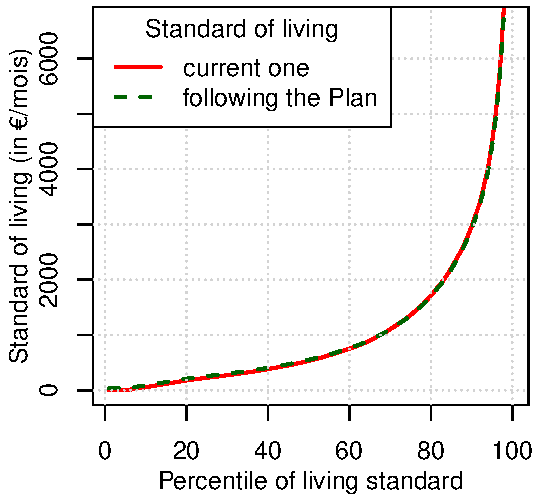
\includegraphics[width=\textwidth]{../figures/policies/gcp_rev_distr_en.pdf}
\end{subfigure} \quad
\begin{subfigure}{.5\textwidth}
  %
  \caption[]{Absolute variation}\label{fig:evol_distr_b}
  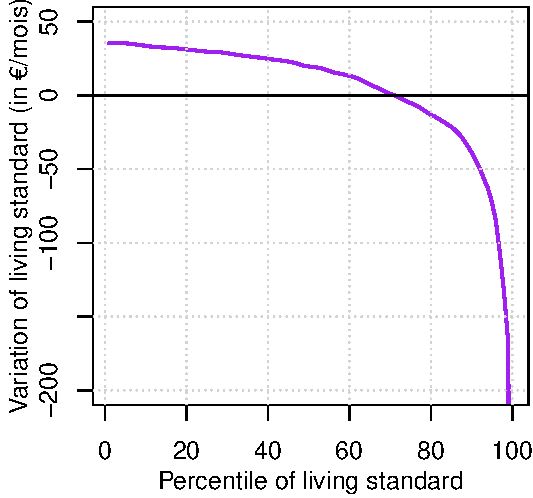
\includegraphics[width=\textwidth]{../figures/policies/gcp_diff_rev_en.pdf}
\end{subfigure}
\quad \quad
\begin{subfigure}{.5\textwidth}
  %
  \caption[]{Relative variation}\label{fig:evol_distr_c}
  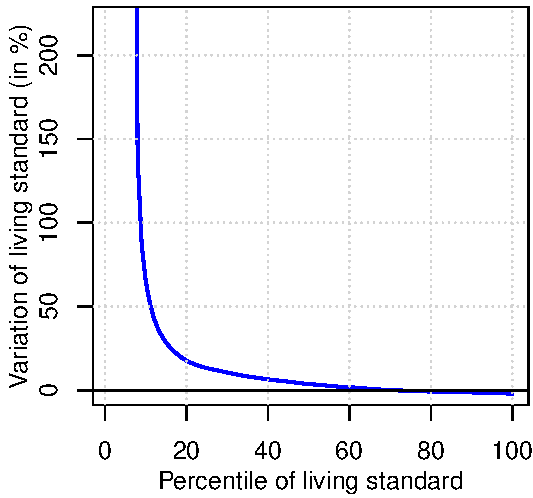
\includegraphics[width=\textwidth]{../figures/policies/gcp_var_rev_en.pdf}
\end{subfigure} \quad
\begin{subfigure}{.5\textwidth}
  %
  \caption[]{Relative variation (top 50\%)}\label{fig:evol_distr_d}
  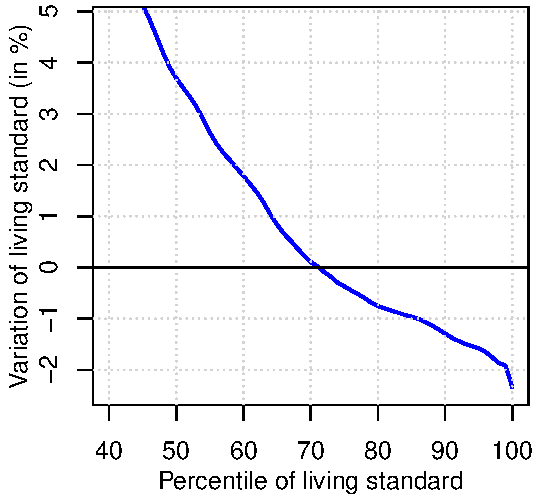
\includegraphics[width=\textwidth]{../figures/policies/gcp_var_rev_rich_only_en.pdf}
\end{subfigure}
{\footnotesize \textit{Note:} Author calculation
(see %methodology in 
Appendix \ref{app:revenus}). Data: carbon footprint by income percentile. Source: Lucas Chancel (World Inequality Database).}
\end{figure}

\section{A majority of winners in most countries}

If the majority of humans end up % SJ would be -> end up
financially better off as a result of the Plan, we might ask what the share of winners would be in each country. Figure \ref{fig:share_below_global_mean} shows these figures, which are equivalent to the proportion of individuals with a carbon footprint below the global average. In India, for example, ninety-four percent of the population would experience a net gain, % SJ there would be 94% winners -> ninety-four percent of the population would experience a net gain,
whereas % SJ while -> whereas
in the EU, % SJ -> comma
it % SJ there -> it
would be just 27 percent. % SJ 27% -> 27 percent.  

Even if the financial loss for the average European caused by the Plan were limited to % SJ would already be limited -> were limited
\euro{}25/month, the Plan would have to be supplemented by national redistribution measures to shift the cost of the ecological transition % SJ moult -> transistion
onto the richest. In Chapter \ref{ch:premier_pas}, I show how a tax increase on the richest %1\% or 
three percent % SJ 3% -> three percent
could finance a transfer that would compensate the typical European or U.S. American, so that they don't lose out financially. Given each country's latitude in distributing the costs of the Plan within its population, the share of winners per country is ultimately less relevant % SJ information -> word deleted
than the distribution of gains and losses between countries, presented below.


\section{A North--South redistribution}

Unsurprisingly, the Global Climate Plan would see a redistribution from the Global North to the Global South. The main contributors would be North America and countries on the Arabian Peninsula, while the main beneficiaries would be sub-Saharan Africa and South Asia. The effects of the Plan country by country can be seen in Figures \ref{fig:gain_2030} (for 2030) and \ref{fig:gain_npv} (for aggregate effects over the whole century). In particular, we can see that, thanks to the participation mechanism mentioned in Chapter \ref{ch:principes}, middle-income countries such as China are neither winners nor losers in monetary terms, compared to the reference situation where decarbonization occurs % SJ takes place -> occurs
at the same pace, % SJ -> comma % 
but without international transfers. 

Obviously, some losing countries like Saudi Arabia or Russia would probably not join the climate union. I have also simulated the Plan's distributional effects in different scenarios where participation would not be universal. Figures \ref{fig:gain_optimist} and \ref{fig:gain_central} present the Plan's effects respectively in an \textit{optimistic} participation scenario and in a \textit{central} scenario. As shown in Table \ref{tab:scenarios_table}, even in a \textit{prudent} scenario (where the union includes only the EU and non-losing countries), % SJ (where the union would include only the EU and non-losing countries) -> where the union includes only the EU and non-losing countries
63\%  %SJ 63% -> 63 percent
of global emissions would be covered. Covered emissions would rise to 74\% %SJ 74% -> 74 percent
in an optimistic scenario in which % SJ where -> in which
most high-income countries join the agreement. While this figure may seem insufficient for a scenario that is supposed to be optimistic, it should be noted that this scenario is above all realistic, since it assumes that the United States would remain outside the climate union, even if the structurally Democratic U.S. states were to join it.\footnote{The structurally Democratic states are those where the Democratic Party won the 2020 presidential election by more than 15 points.} Let's hope % SJ wager -> hope
that these partial participation scenarios will only be valid in the short term, and that the Plan will bring together a critical mass of countries, sufficient to establish a global social norm in favor of the climate union, which will push all countries to join it in the long term.

\clearpage
\begin{figure}[h] %\vspace{-.5cm}
  \caption[Share of winners by country]{Share of winners following the Plan, by country.}\label{fig:share_below_global_mean}
  \centerline{
    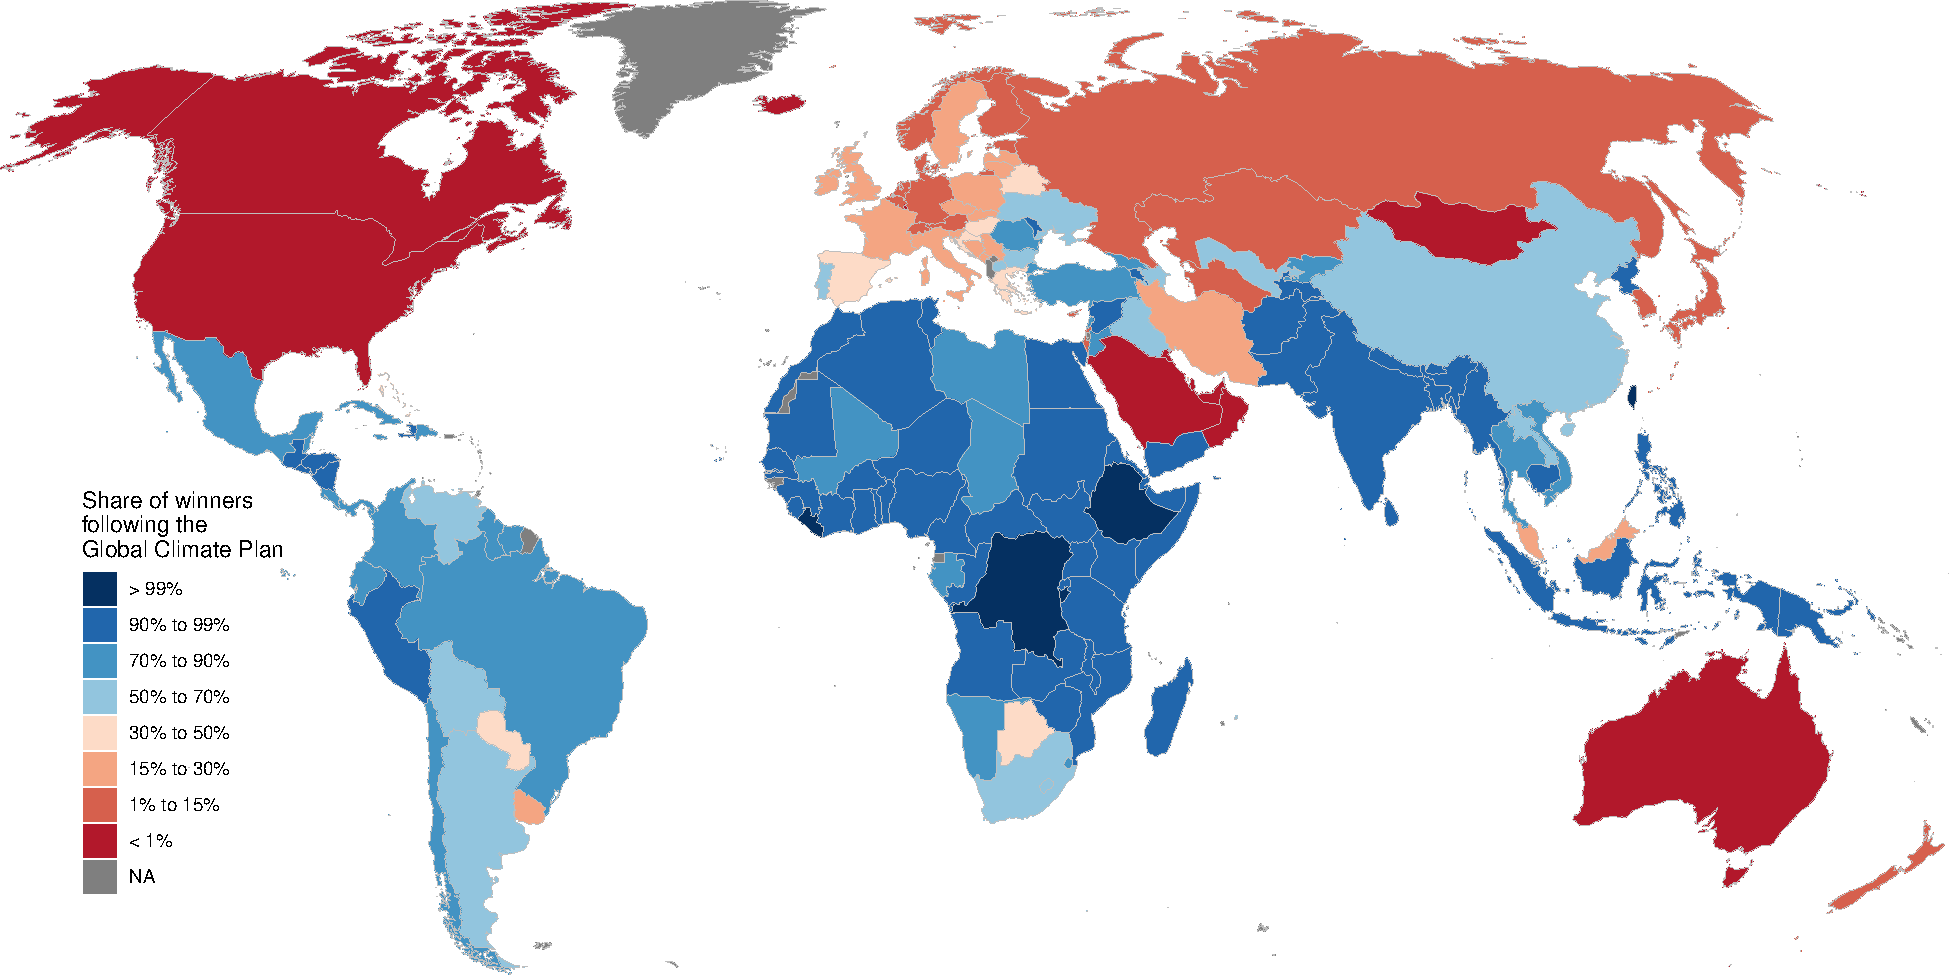
\includegraphics[width=.8\paperwidth]{../figures/maps/share_below_global_mean_en.pdf}
    } 
 {\footnotesize \textit{Note:} Is considered a winner anyone with a carbon footprint below the global average. Source: \href{http://wid.world}{wid.world}.
 }
\end{figure} 
\begin{figure}[h] %\vspace{-.2cm}
  \caption[Net gains by country in 2030]{Monetary gains or losses by country as a result of the Global Climate Plan, in 2030.}\label{fig:gain_2030}
  \centerline{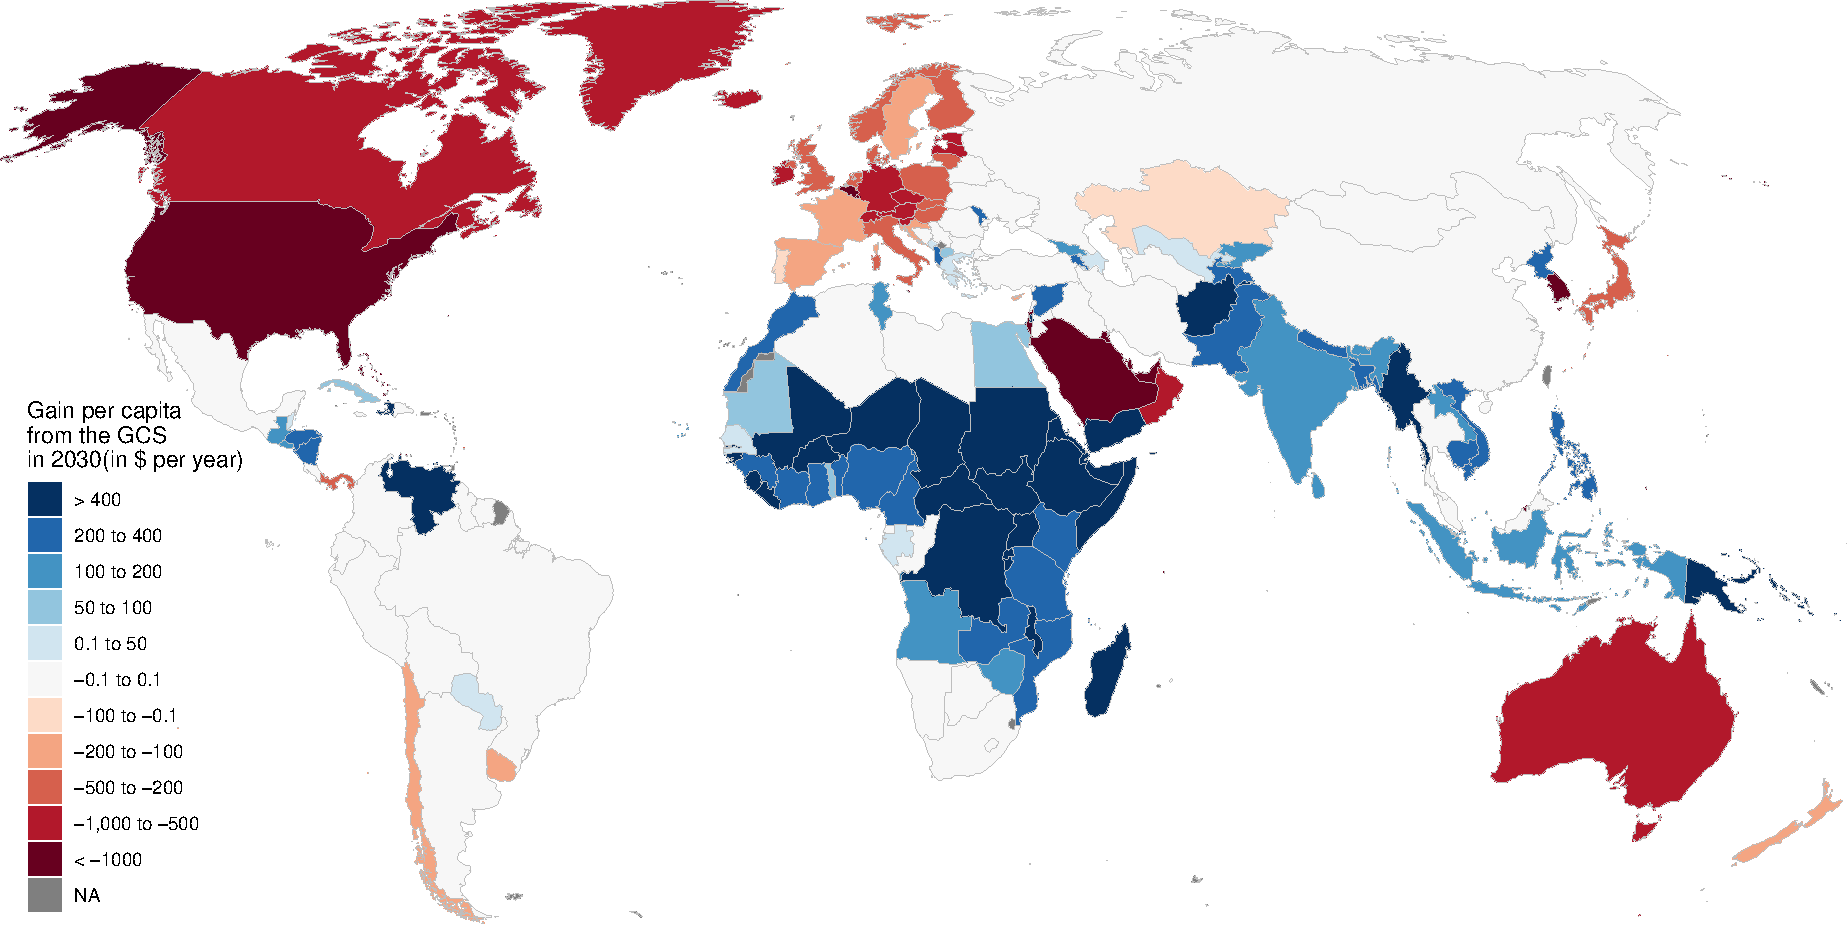
\includegraphics[width=.8\paperwidth]{../figures/maps/gain_adj_2030.pdf}}  \vspace{-3cm}
\end{figure}

\begin{sidewaysfigure}
  \caption[Net gains by country over the XXI$^\text{e}$ century]{Monetary gains or losses as a result of the Global Climate Plan over the XXI$^\text{e}$ century.}\label{fig:gain_npv}
  \centerline{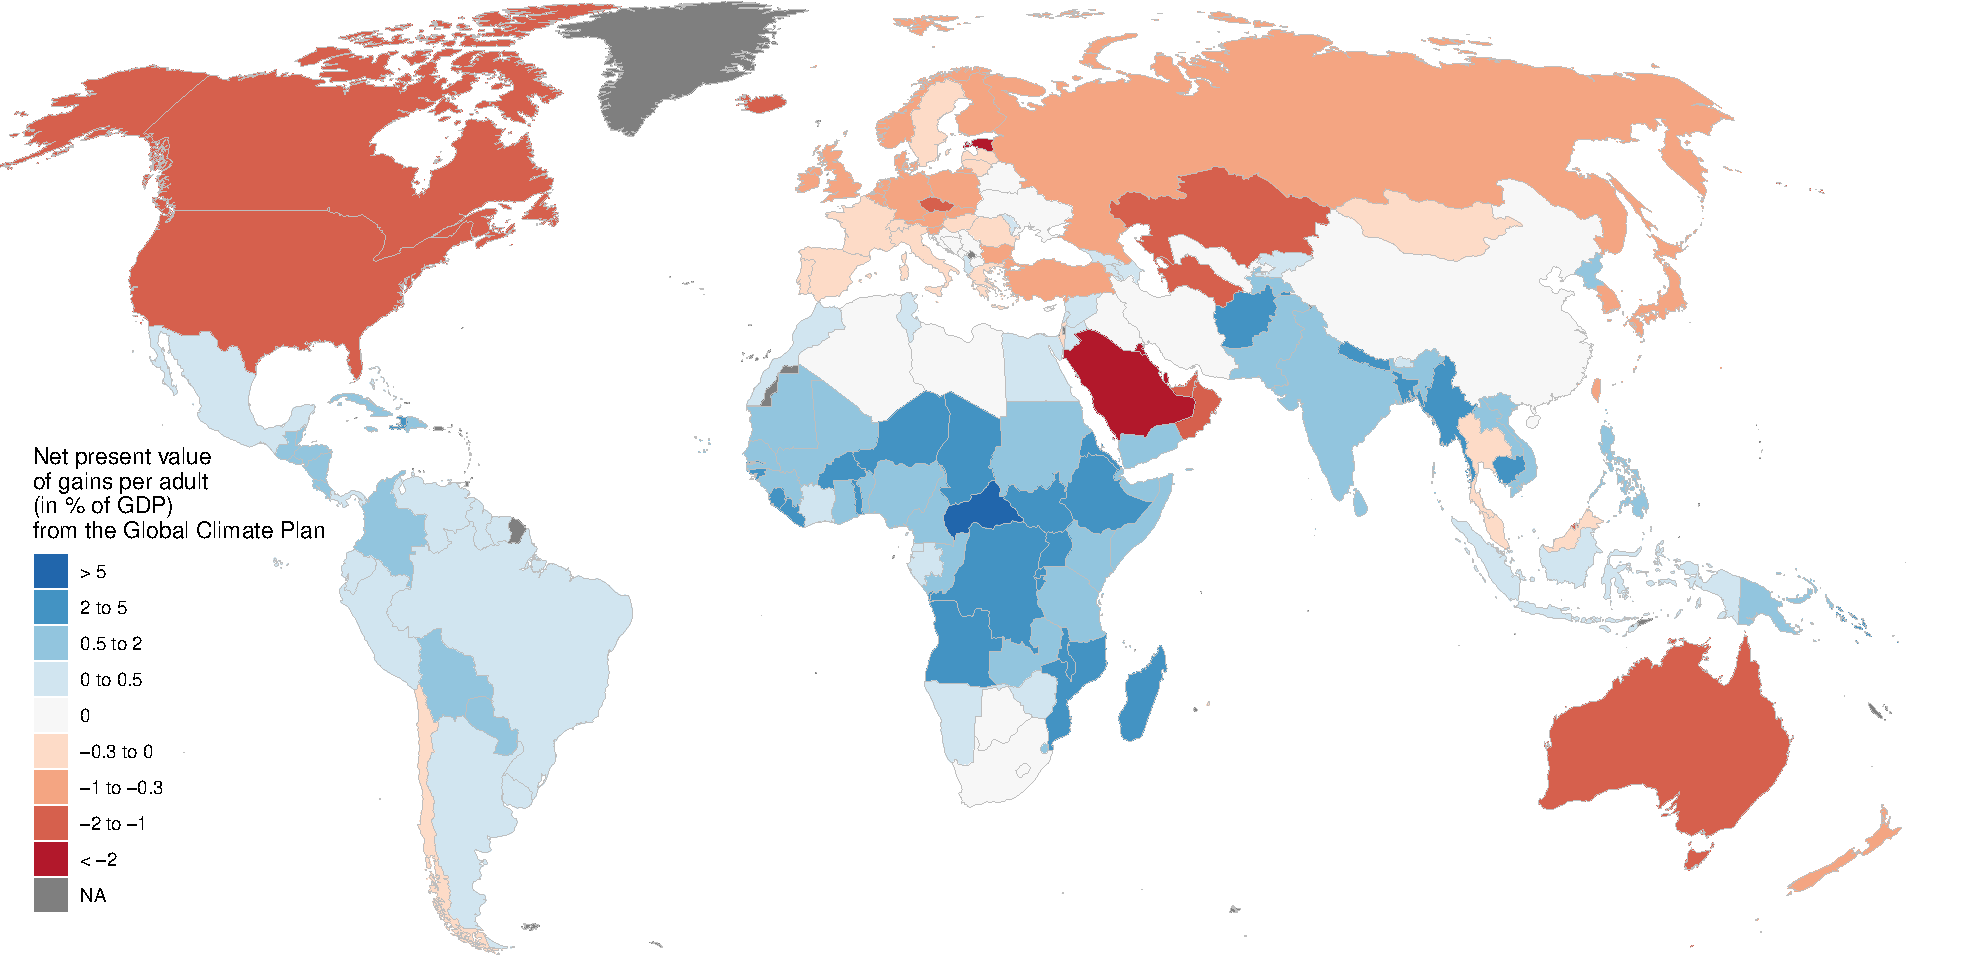
\includegraphics[width=.9\paperheight]{../figures/maps/npv_over_gdp_gcs_adj.pdf}
    } %
  {\footnotesize \textit{Note:} The net present value is calculated using a discount rate of 3\% over the period 2030--2100}.
\end{sidewaysfigure}

\begin{figure}[h!]
  \caption[Net gains in an \textit{Optimist} participation scenario]{Monetary gains or losses by country following the Plan in an \textit{Optimist} participation scenario.}\label{fig:gain_optimist}
  \centerline{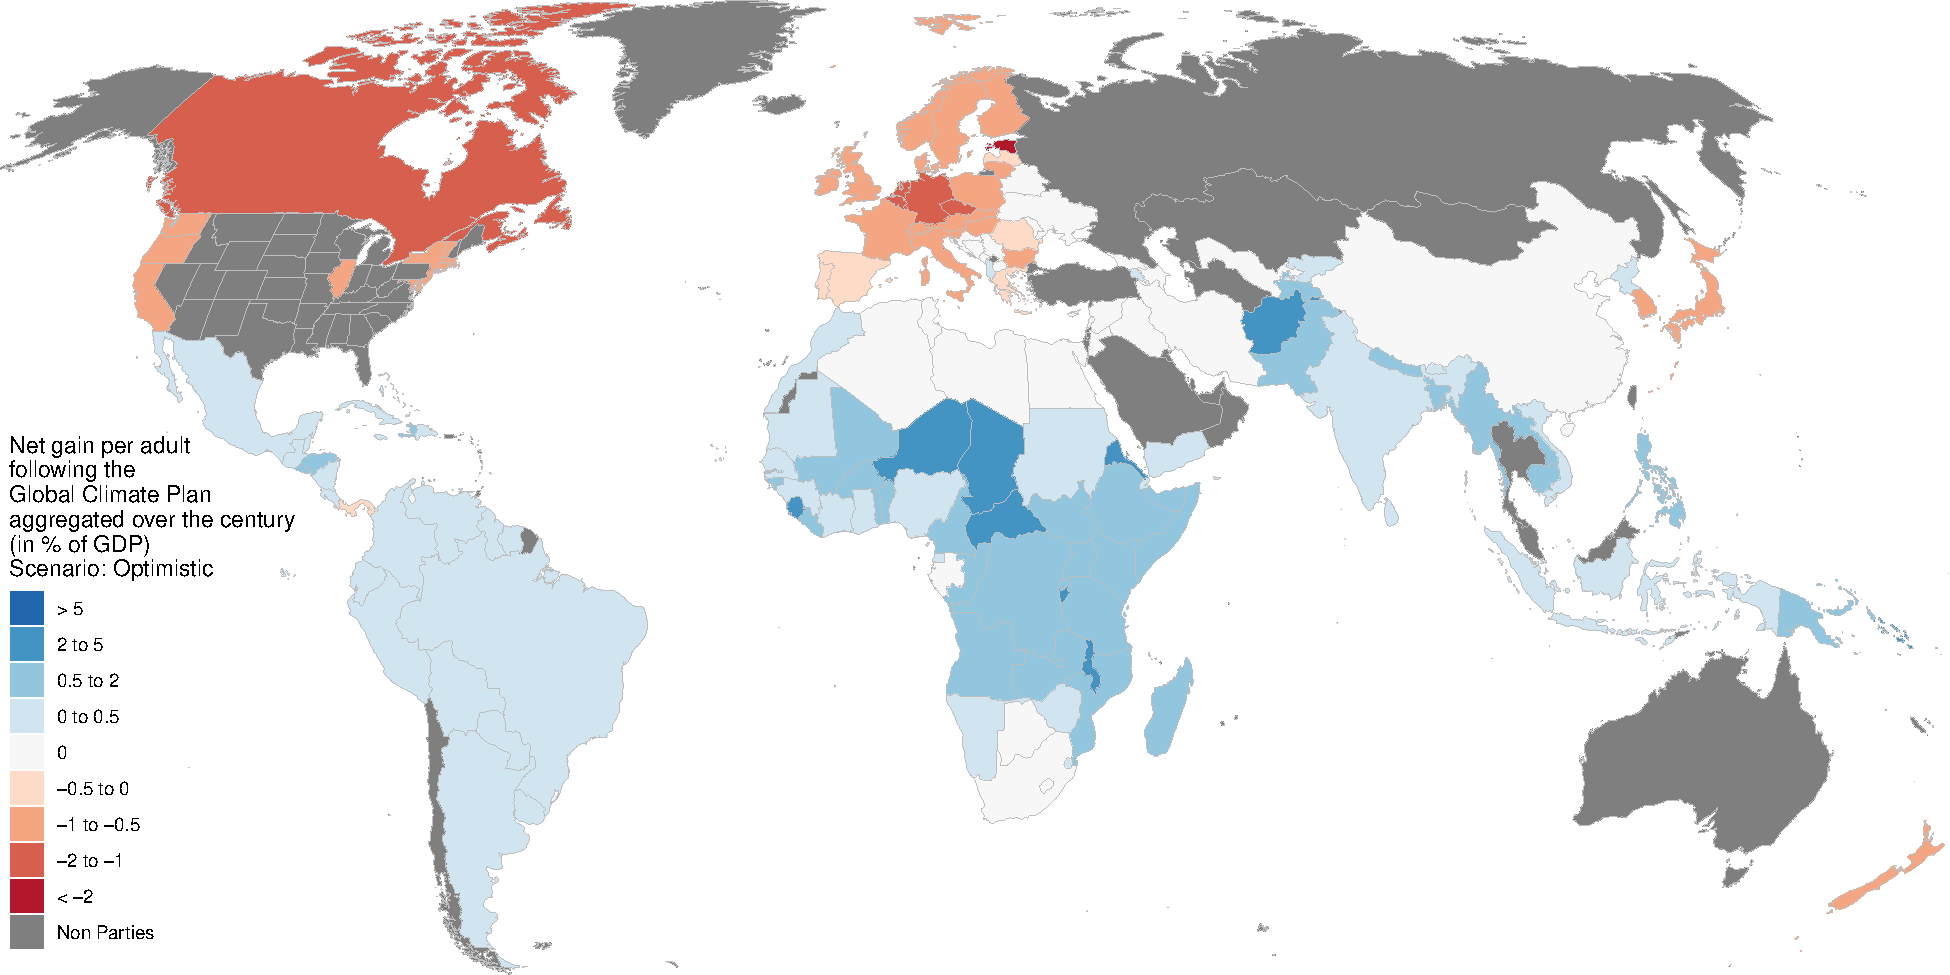
\includegraphics[width=.85\paperwidth]{../figures/maps/Soptimistic_npv_over_gdp_gcs_adj.pdf}} 
\end{figure}
\begin{figure}[b!]
  \caption[Net gains in a \textit{Central} participation scenario]{Monetary gains or losses by country following the Plan in a \textit{Central} participation scenario.}\label{fig:gain_central}
  \centerline{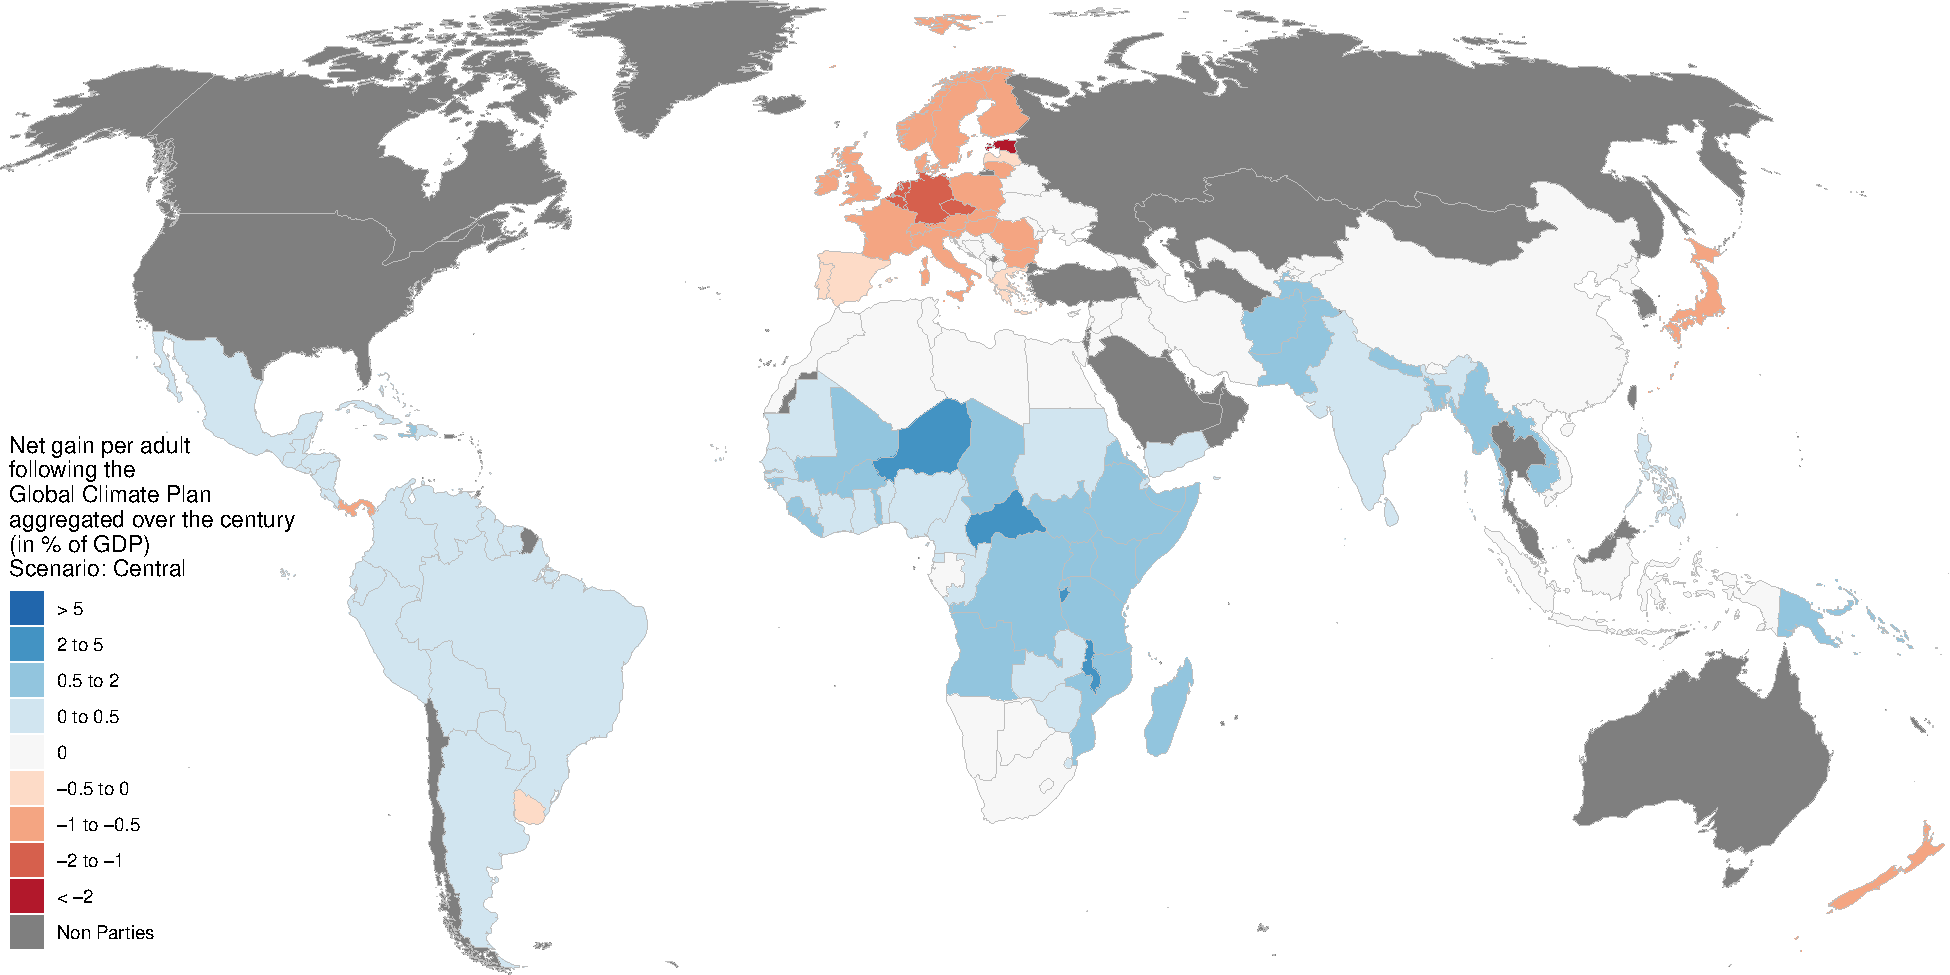
\includegraphics[width=.85\paperwidth]{../figures/maps/Scentral_npv_over_gdp_gcs_adj.pdf}
    } 
\end{figure}

\chapter*{\textit{The concrete effects of the Plan on people's lives}}\label{ch:narr_bilan}
\addcontentsline{toc}{chapter}{\nameref{ch:narr_bilan}} 

Seven years after the Global Climate Plan came into force, three-quarters of India's coal-fired power plants are shut down. % SJ Seven years after the Global Climate Plan came into force, three-quarters of India's coal-fired power plants are shut down -> Seven years after the Global Climate Plan comes into force,  India has shut down three-quarters of it's coal-fired plants.
Firstly % SJ Firstly -> By now, coal
has become % SJ is now -> has become
 more expensive than gas, since it contains twice as much CO$_\text{2}$. This makes it cheaper to generate electricity from gas-fired power stations. Above all, electricity from renewable sources is even cheaper, and it is developing fast. Indeed, in anticipation of the Plan, the Indian government has invested heavily in the deployment of wind power and solar panels. In just seven years, the proportion of electricity generated from renewable sources has risen from 20\% to 80\%. As a result, Indian emissions have fallen by 30\% over the period, and air pollution has been reduced significantly. % SJ significantly reduced -> reduced significantly. 

Rajesh is a cab driver in Calcutta. He's done the math: an electric car now costs the same as a combustion-engine car, when you factor in the price of fuel. Charging stations have been widely installed in the city, and the price of petrol will continue to rise. Rajesh has made up his mind: the next time his old car breaks down, he will get rid of it and invest in an electric Tata. Rajesh earns around \euro{}300 a month, of which \euro{}50 is basic income. Thanks to this stable income, Rajesh was able to borrow money to buy a second-hand car. %
Before becoming a cab driver, he sold samoussas on the street and earned half as much, just enough to live in a small room. Although his monthly expenses have risen by 25\euro{} with inflation, he and his wife can now afford a nice three-room apartment, which they have just moved into with their newborn daughter. Thanks to the basic income, he no longer needs to send money home to his family in the countryside, and he can attend a monthly cricket match with his favourite team. 

Jordan, on the other hand, is upset by this Global Plan. He lives in Vancouver, but his closest family and friends live in Ottawa, where he grew up. Yet the price of a round-trip flight has risen from \euro{}250 to \euro{}400. Jordan would not give up his monthly weekends in his hometown for anything in the world. So he had to cut back on the rest. Jordan did not renew his gym membership --- he's now content with jogging and floor exercises at home, and he lowered his apartment thermostat a little (from 23 to 21\textdegree{}C) to save money. From what he's read in the papers, the price of a ticket is set to rise to \euro{}800 in twenty years' time, when planes will be powered by hydrogen. Never mind, Jordan swears he will continue to make the trip just as frequently, even if it means moving to a cheaper neighborhood if he needs to free up more purchasing power. And to hell with his colleagues urging him to join the self-limitation movement, he won't give in to this sanctimonious fad!

Rosalie, for her part, is all smiles. Thanks to a tontine system, her neighborhood has joined forces to buy a shared tractor. The work in the fields is much easier, and the hours much shorter, since the arrival of the machine. Since the payment of the basic income, construction work has been non-stop in Houndé. Electricity companies are laying cables in every street, the town hall is installing public latrines, not to mention the brand-new hospital paid for by the Burkinabe government. Of the \euro{}50 Rosalie receives each month on her phone, \euro{}20 goes directly to taxes (half to the town, half to the state), and \euro{}10 % goes to the government.
in the tontine. With the \euro{}20 she has left, Rosalie first treated herself to a mattress, taking out a one-year loan with her husband. She now has much less back pain. Above all, she always has enough to buy vegetables and rice. She and her family will never have to go hungry again.


\chapter{A step towards a sustainable world}\label{ch:premier_pas} %

  % SJ  
The proposed Plan % SJ The proposed Plan -> The Plan I have proposed
is just one of the building blocks needed to create a sustainable world. It is not the object of this book % SJ It is not the object of this book -> The objective of this book is not
to detail an exhaustive set of measures for achieving a harmonious society. However, even if it can be negotiated independently of the rest, the Global Climate Plan should not be thought of in isolation, but as part of a system of mutually reinforcing measures. In this chapter, I % SJ we -> I
provide an overview of complementary measures to the %SJ our -> the/my
Plan, at both %SJ -> a
a global and % SJ -> a
a national level. On the %SJ a -> the
global scale, the Plan should be complemented by democratic governance and other measures of North--South redistribution. At the % SJ -> the
national level, the ecological transition %SJ moult -> transition
should be accompanied by more redistributive taxation and sectoral climate policies. 

\section{For a truly sustainable world}

\subsection{The need for additional redistribution}
In a country like Burundi, where GDP \textit{per adult} is around \euro{}450 per year and CO$_\text{2}$ emissions 0.1 tonne per year, the %SJ our -> the
Plan, % SJ --- -> comma
and its basic income of \euro{}50 per month per adult, % SJ --- -> comma
would double the average income. 
However, with an average \textit{per capita} income of around \euro{}50 per month --- or \textit{\texteuro{}}130 per month adjusted for the cost of living,\footnote{As a reminder, we denote the euro in purchasing power parity by the italicized sign \textit{\texteuro{}}.} 
living standards would remain insufficient for most Burundians. More global redistribution is needed to ensure a decent life for everyone. 

It takes at least \textit{\texteuro{}}7 a day to have a decent life in a Global South country.\footnote{It is not easy to define a monetary threshold corresponding to the minimum required for a decent life. Based on the work of \cite{oneill_good_2018}, Jason \cite{hickel_is_2019} measures the attainment of 11 social indicators in each country: healthy life expectancy of at least 65 years, 2,700 kcalories per person per day, secondary school enrolment, access to electricity, sanitation, and so on. He shows that in a country like Sri Lanka, social indicators are almost universally respected, and that they could be perfectly so with the help of additional national redistribution. We can deduce from this that the average Sri Lankan income of \textit{\$}250 
per month, %.
is enough to ensure a decent life in this country. Furthermore, \cite{kikstra_decent_2021} show that \textit{\$}210 per month %.
is generally insufficient for a decent life, defined according to equivalent criteria. Thus, the monetary threshold enabling basic needs to be met is probably between \textit{\$}210 and \textit{\$}250 per month (on average in Global South countries), or between \textit{\$}6.85 and \textit{\$}8.25 per day. In the absence of any academic study calculating such a threshold, I will use the intermediate value of \textit{\$}7.5 (or {\texteuro{}}7) per day as the poverty line.} 
By 2030, an estimated 40\% of the world's population will be living on less than that. %
It would then cost 2\% %.
of global GDP to eradicate poverty defined at a threshold of \textit{\texteuro{}}7 per day\footnote{The poverty rate was calculated for 2030 from data from the \textit{Poverty and Inequality Platform}, assuming global growth of 3.5\% per year between now and then. The extent of poverty in dollars was calculated from the same source and divided by global GDP using World Bank data, with the same growth assumption.} 
by providing each poor person with the income that separates them from this threshold. This figure is consistent with the cost of the investments needed to achieve the Sustainable Development Goals (which largely overlap with the social indicators of a decent life), estimated at around 2\% of world GDP by the \citet{unctad_estimating_2021}. %
The basic income financed by the Plan would transfer around 1\% of world GDP to poor people.\footnote{In fact, the poorest 40 percent % SJ 40% -> 40 percent
of humans currently get 5.1\% of world income, and this share would rise to 6.0\% following the Plan, according to the methodology in Appendix \ref{app:revenus}. As shown in Table \ref{tab:gcp_ineq}, more than half (but not all) of this transfer would reduce the gap separating poor people from the poverty line, with the remainder making certain incomes increase above the poverty line. Thus, it would still take 1.6\% of world GDP to eradicate poverty after the Plan, and we can consider that a third of this sum could be financed by low-income countries themselves.} Therefore, 
additional revenues of at least 1\% of global GDP would be needed to end poverty. %

\subsection{A global tax on wealth} %
There are several ways of raising such a sum. The most promising is undoubtedly the wealth tax. First of all, the wealth tax also fulfills another objective, since it can be presented as a means of settling 
historical responsibility for climate change, rather than as a measure of solidarity. It is generally accepted that rich countries are historically responsible for climate change. However, it may be more fruitful to attribute this responsibility to wealthy individuals. % SJ people -> individuals
Indeed, it seems that people who have inherited assets built on fossil fuels benefit more from past emissions than, for example, a typical Ukrainian, born in a country that used to pollute a lot but has since become impoverished.\footnote{In 2022, Ukraine's GDP per capita in purchasing power parity is 35\% below its 1990 level (and was already 21\% lower in 2021), according to the \href{https://data.worldbank.org/indicator/NY.GDP.PCAP.PP.KD?locations=UA}{World Bank}.} %
Based on the work of \cite{fanning_compensation_2023}, I have calculated that the compensation owed by rich countries for emissions from the 1990--2030 period amounts to a staggering % SJ -> a staggering
26,000 billion dollars, or 25\% of world GDP.\footnote{\cite{fanning_compensation_2023} estimate at 192,000 billion dollars the compensation due by rich countries for having exceeded the emissions quota proportional to their population and corresponding to a warming scenario of 1.5\textdegree{}C. This estimate is obtained by multiplying cumulative emissions over the period 1960--2050 (assuming rapid decarbonization by 2020--2050) %.
with a carbon price trajectory over 2020--2050 corresponding to the 1.5\textdegree{}C scenario. The universal implementation of the Global Climate Plan in 2030 would put an end to the need to offset excess emissions from this date onwards, since these would already be priced in. % SJ -> in
So, to calculate the compensation due for the period 1960--2030, we can use the cumulative emissions over this period and the average carbon price over the period 2020--2030 (i.e. 135\$/tCO$_\text{2}$) rather than 2020--2050 (288\$/tCO$_\text{2}$). This would give 75,000 billion. However, the assumptions of \cite{fanning_compensation_2023} can be challenged as being too radical: the dangerousness of % SJ dangerousness of -> threat posed by
climate change was only universally recognized in 1990, and the target on which countries have unambiguously agreed is a warming of 2\textdegree{}C rather than 1.5\textdegree{}C. Considering a 2\textdegree{}C scenario over the period 1990--2020 (or alternatively, taking the initial assumptions with a price of 45\$/tCO$_\text{2}$), we obtain 26,000 billion. These calculations can be reproduced on \href{https://github.com/bixiou/compensation-atmospheric-appropriation}{github.com/bixiou/compensation-atmospheric-appropriation}.} 
By attributing this debt to multimillionaires and spreading its repayment over the future, we end up with a flow from rich to poor of the order of just % SJ -> just
1\% of world GDP.\footnote{It is financially equivalent to transferring % SJ transfer -> transferring
capital directly or to paying % SJ pay -> paying
out the annual return on this capital forever. Assuming a credible rate of return on the % SJ -> the 
capital of % SJ -> of
4 percent, % SJ 4% -> 4 percent no brackets
a debt of 25 percent % SJ 25% -> 25 percent
of world GDP can therefore be converted into an annual flow of 1\% of world GDP.} 
Apart from addressing the historical responsibility for climate change, there are two other advantages to a wealth tax. Primarily, % SJ On the one hand -> primarily
such a tax exists in only a handful of countries, and can therefore be set up to finance third countries without encroaching on existing national budgets. Secondly, this tax has the potential to collect the large revenues we are looking for, while sparing the average person. %

For example, the sum of 1\% of world GDP could be collected by a global tax that would tax individual wealth at a rate of 2\% per annum % SJ (per annum) -> per annum
from 5 million.% upwards.
\footnote{
The \href{https://wid.world/world-wealth-tax-simulator/}{wid.world/world-wealth-tax-simulator} website developed by \cite{chancel_world_2022} allows you to simulate the tax scale of your choice.} %
With such a scale, the 99.9\% of people who own less than 5 million in assets would not pay any tax, and a person owning 10 million would pay 1\% tax on their % SJ her -> their
wealth.\footnote{In effect, the tax would be 2\% on their % SJ her -> their
wealth above 5 million, or 2\% of $10-5=5$ million, which in relation to 10 million corresponds to 1 percent of their wealth  % SJ --- in relation to 10 million --- corresponds to 1\% -> in relation to 10 million corresponds to 1 percent of their wealth.
} 



\subsection{Towards a more radical redistribution}
Such a tax would therefore not be revolutionary: it would not prevent the emergence or maintenance of billionaire fortunes, whose returns are generally in excess of 7\%.\footnote{\cite{chancel_world_2022}.}  
This moderate approach would win the support of a large majority of the population. However, a society that maintains both billionaires and people living on \textit{\texteuro{}}7 a day would be far from socially just. To achieve a truly sustainable world, we would need much less inequality. % SJ : -> .
For example, we might consider that the highest income should be limited to five times the minimum income (a standard attributed to the very first ``Nobel Prize'' in economics, Jan Tinbergen). So, the proposals put forward in this book are just one step towards a sustainable world. The road is a long one because infrastructures and social structures do not change overnight, % SJ --- because infrastructures and social structures do not change overnight --- -> because infrastructures and social structures do not change overnight,
but it is worth it.  

Not only do we have to go down this road, we also have to make sure we don't go backwards. And that's % SJ that's -> that is exactly
what could happen if we don't take further measures to complement our Plan, when decarbonization comes to an end. %
At that point, the revenues linked to the carbon price will collapse. It would be disastrous if the basic income were to collapse alongside it. % SJ  with them -> alongside it.
We will need new resources % SJ New resources will therefore be needed -> We will need new resources
to maintain, or even increase  % SJ maintain (or even increase) -> maintain, or even increase
the basic income, 
from taxes on wealth, high incomes or companies. 

\subsection{The other global projects to be undertaken}
Global redistribution is not the only thing that needs to be done --- far from it. % SJ --- far from it. -> ; far from it!
Worldwide % SJ Global -> Worldwide
democracy is another. %
Indeed, all decisions should be taken at the relevant level, in accordance with the principle of subsidiarity. This means that decisions with global repercussions must be taken on a global scale. %
This is notably the case for decisions relating to climate change, pandemics, artificial intelligence and the financial system. %
The precise form of global governance has yet to be defined, but it must be democratic, if inequalities in decision-making power are to be considered as unfair as inequalities in wealth. %

In addition, the Plan should be supplemented by other international treaties on uncovered greenhouse gases such as methane, % SJ (such as methane) -> such as methane
land use and deforestation. 

Finally, we need to adapt the international financial system to make it more advantageous to % SJ for -> to
developing countries. In particular, decarbonization % SJ decarbonisation UK
requires the development of \textit{climate finance}, i.e. the financing of low-carbon projects. The financing of projects in low- and middle-income countries is hampered by the disadvantageous and risky conditions they face: high interest rates, exchange rate volatility and the  unsustainability % SJ , unsustainability -> and the unsustainability
of public debt.  % SJ debt\dots{} -> debt.
Numerous proposals have been made, notably by the United Nations General Secretariat and the Green Climate Fund:\footnote{Cf. \href{https://www.un.org/sustainabledevelopment/blog/2023/04/press-release-with-clock-ticking-for-the-sdgs-un-chief-and-barbados-prime-minister-call-for-urgent-action-to-transform-broken-global-financial-system/}{Bridgetown Initiative 2.0}, \href{https://www.greenclimate.fund/sites/default/files/document/scaling-climate-finance-context-covid-19-full-report\_0.pdf}{Scaling Climate Finance}, \citet{hourcade_accelerating_2021}.} public guarantees on credit and foreign exchange markets, recapitalization of multilateral development banks, cancellation of public debt, issuance of climate remediation assets, increased inter-state lending and allocation of Special Drawing Rights. Behind these technical mechanisms lies a simple idea: to provide the funds and guarantees needed to finance the ecological transition. % SJ moult -> transition
These mechanisms are often based on relatively painless bookkeeping arrangements, which basically involve creating money to finance low-carbon projects. Under pressure from Global South countries, these initiatives are making progress, but % SJ but -> but they are moving
too slowly in relation to the needs.


\section{For a smooth transition % SJ moult -> transition
in every country}\label{sec:mue_nationale}

In low-income countries, the establishment of a % SJ the -> the establishment of a
basic income will represent a considerable influx of resources, and will greatly increase the capacity of states to raise taxes. With the help of progressive income taxes, among other things, % SJ taxes (among other things) -> taxes, among other things
these states could increase their budgets and finance public services, social protection and new % SJ and -> and new
infrastructure. In these countries, only the wealthiest people, those with a carbon footprint above the global average, % SJ --- those with a carbon footprint above the global average --- ->, those with a carbon footprint above the global average,
would lose out financially. 

\subsection{A national redistribution} %
Conversely, % SJ On the other hand, -> Conversely,
in high-income countries, most individuals would lose some % lose -> lose some
purchasing power in the absence of additional measures. Of course, richer people would lose more, as they have a higher average carbon footprint. However, it would be both unfair and unpopular for the middle classes to suffer a drop in their standard of living if the well-off can cope with price rises on carbon-intensive goods simply by dipping into their savings or cutting back on a few superfluous expenses. To avoid this inequality, the ecological transition % SJ moult -> transition
must be accompanied by redistribution in high-income countries. The contribution of the most affluent would fulfill % SJ fulfill -> fulfil
three roles: compensating the middle classes to prevent them from losing out financially, financing low-carbon infrastructures to avoid passing the cost on to unlucky groups,(such as households heated with oil), % SJ groups (such as households heated with oil) -> groups, such as households heated with oil,
% and reducing the cost of carbon emissions.
and reducing, or even eliminating completely, % SJ and the reduction (or even elimination) of -> and reducing or even eliminating completely
superfluous, high-emission activities that undermine social cohesion.

In the European Union, increased taxes on the richest 1\% would be enough to offset the typical person. % SJ persone -> person
Thus, an  eight point % SJ a 8-point -> an eight point
increase in the tax rate on individual incomes above \euro{}10,000 per month would finance a transfer of \euro{}25 per month to each European, preventing the typical European from losing purchasing power as a result of the Plan. Such a transfer could be achieved by raising minimum social benefits and slightly reducing income tax for 99\% of the population. But it might be better to make this transfer in kind, by financing public education and health services. In the United States, where carbon footprints are much higher, a more substantial redistribution would be needed to compensate the typical U.S. American. Such compensation would require a transfer equivalent to \$140 per month to each U.S. American, which can also be financed by an increase in tax rates for the richest 3\%, those earning more than \$25,000 per month.\footnote{Such a transfer could be financed by taxing capital gains and profits as income, and raising the marginal tax rate from 32\% to 33\% for annual incomes between 315,000 and \$400,000, from 35\% to 40\% between \$400,000 and \$600,000, from 37\% to 50\% between \$600,000 and \$5 million, and from 37\% to 60\% above \$5 million. The scale is based on the simulator \href{https://taxjusticenow.org/}{taxjusticenow.org} from \cite{saez_triumph_2019}.}%.

Low-carbon equipment  such as public transport, thermal renovation % SJ (public transport, thermal renovation, etc.) ->  such as public transport, thermal renovation
and loss of revenues from fossil fuel taxation % SJ taxes on fossil fuels -> fossil fuel taxation
can also be financed by additional taxes on the wealthiest\footnote{In addition to the Global Climate Plan, the other measures discussed in this chapter require the redirection of around 4\% % SJ 4\% -> 4 percent
of global GDP, 2 percent  % SJ 2\% -> 2 percent
of which could finance carbon sequestration and a global basic income once decarbonization is complete. %
This cost could be borne entirely by the richest 1\% of human beings, those earning over \euro{}10,000 per month, % SJ (those earning over \euro{}10,000 per month), -> ,those earning over \euro{}10,000 per month,
who account for around 16\% of after-tax income. To achieve this, it would be sufficient to increase the tax rate on income above \euro{}10,000 per month by 15 points, and to make the wealth tax mentioned above more progressive, by raising the marginal rate to 6\% on wealth above 100 million and to 10\% above 1 billion. Income tax revenues are estimated on the basis of the average world income (\textit{\texteuro{}}1,550/month) and the average income of the top 1\% (\textit{\texteuro{}}30,000/month) given by the \href{https://wid.world/data/}{WID}; and those of the wealth tax on the basis of the \href{https://wid.world/world-wealth-tax-simulator/}{WID} simulator.
} (see Table \ref{tab:redistr_policies}). 
For example, an income tax schedule more progressive than the one mentioned above would make it possible to collect the additional percentage of GDP needed to finance decarbonisation.\footnote{\citet{aie_net_2021}.} 

\begin{table}[h]
  \caption[Redistribution measures]{\label{tab:redistr_policies}Six redistribution measures, each collecting about 1\% of global GDP.}.
  \makebox[\textwidth][c]{
  \begin{tabular}[t]{cccc}
  \toprule
  \makecell{Measure} & Variant & \makecell{Usage,\\effect} & \makecell{North--South\\Transfers} \\
  \midrule
  \multicolumn{2}{c}{Global Climate Plan} & \makecell{Global basic income,\\End extreme poverty} & $\checkmark$ \\[1em]
  \multirow{2}{*}{\makecell{Global\\Wealth\\Tax}} & \makecell{2\% rate\\above \euro{}5~M} & \makecell{Public spending (in the Global South),\\End poverty and repay the climate debt} & $\checkmark$ \\[0.9em]
    & \makecell{Progressive rates\\above \euro{}100~M} & \makecell{Compensation of fiscal revenue loss\\from taxes on fossil fuels} & \\[1em]
  \multirow{2}{*}{\makecell{Hike in\\income\\tax\\above:}} & \makecell{\euro{}20,000/month} & \makecell{Green investments\\then carbon sequestration} & $\sim$ \\[0.9em]
  & \makecell{\euro{}10,000/month} & \makecell{Compensation of the middle class\\then basic income} & $\sim$ \\[0.9em]
  & \makecell{\euro{}6,000/month} & \makecell{Improved public services} & \\[0.2em]
  \bottomrule\\[-0.81em]
  \end{tabular}}
  \footnotesize{Note: $\sim$ means North--South transfers only at the end of the century}.
\end{table}

Finally, in order to achieve a more % SJ with a view to an -> in order to achieve a more
egalitarian transformation of society, certain superfluous items of consumption could be banned outright, such as yachts or private jets. In fact, we could even consider that above a certain income, consumption is necessarily superfluous, and cap incomes at this level. This level could be determined each year by taking the median preference of a representative sample of citizens. In a representative survey of a thousand French people, a majority favored % SJ favoured UK
the introduction of a legal maximum income, with a preferred value of \euro{}100,000 per month as the median.\footnote{To calculate the median, the 44\% not wishing to impose a legal maximum income were treated as preferring an infinite value. The remainder reported the amount of their choice. A variant of the question asked respondents what the maximum income would be in an ideal society: only 16\% replied that there would be no limit, and the median was then \euro{}15,000 per month \citep{fabre_determiner_2022}.} 

As you can see, I am in favor % SJ favour UK
of sharply limiting inequalities, and convinced that ecological constraints will be better accepted in a less unequal society. I would also support % SJ I am also in favor of -> I would also support
a global agreement on the taxation, or even capping % SJ (or even capping) -> , or even capping
of large fortunes, to prevent tax evasion. However, most of the redistribution measures I have just proposed can be decided at national level, according to the sensitivity of each people, so that the choice of the level of redistribution does not complicate the adoption of the Global Climate Plan. The Plan only determines the  trajectory of global decarbonization  % the global decarbonization trajectory -> the trajectory of global decarbonization / decarbonisation UK
and the transfers from polluters to the frugal, and preserves the sovereignty of each State to implement the appropriate complementary measures.

\subsection{National climate measures} %{National climate measures} %{National climate measures

There are also a number of reasons why we need additional climate policies. % SJ In particular, additional climate policies are needed for a number of reasons. -> There are also a number of reasons why we need additional climate policies.
Firstly, the public authorities have the competence to plan the territory and the capacity to take charge of long-term investments: rail network, public transport, low-carbon energy and thermal renovations. % SJ energies, thermal renovations -> energy and thermal renovations. 
Secondly, to ensure that private choices of investment, equipment and R\&D %SJ (of investment, equipment, R\&D) -> of investment, equipent and R\&D
are aligned with our values and with planned long-term decarbonization % SJ decarbonisation,
the State must define standards, whether for emissions from new vehicles, the energy efficiency of new buildings or animal husbandry. %
Thirdly, the assumption of decarbonization % SJ decarbonisation UK
costs by public authorities helps to spread the financial effort more evenly and combat the so-called ``horizontal'' inequality arising from the wide variation in carbon footprints for the same level of income. %

Because of this horizontal inequality, the application of the polluter-pays principle through the carbon price results in disparities in the effects on purchasing power. For example, % SJ power: -> power, For example, 
someone who heats with oil and drives to work will lose much more than someone who lives in a well insulated home and commutes by bike. 
These horizontal disparities are not always justified, insofar as individuals are penalized when alternatives to fossil fuels are often non-existent or unaffordable, due to collective or past choices for which they bear little responsibility (single-family homes, thermal boilers, etc.). By pooling decarbonization % decarbonisation UK
costs such as thermal renovation and the replacement of an oil-fired boiler with a heat pump, someone who heats with electricity in a well-insulated house will, thanks to tax-financed subsidies, be helping people living in a poorly-insulated, oil-heated house. 

Emissions reductions due to complementary climate policies in certain countries 
will produce four effects: a reduction in horizontal inequality in these countries, a fall in emissions in these countries, a fall in the global carbon price,\footnote{Let us take an example to understand. 
To encourage people to renovate their homes and replace their gas boiler with a heat pump, we can either raise the carbon price (and therefore fuel oil), or subsidize the work. 
Subsidies reduce the cost of the work, thus lowering the carbon price at which it becomes profitable. 
If many countries subsidize this type of work, demand for emissions permits is reduced, as is the carbon price. 
A boiler ban would force homeowners who need to replace their boilers to use a non-fossil fuel energy source, and would also lower the demand for emissions permits, and the carbon price with it. More generally, all complementary climate policies reduce the carbon price.} 
and a reduction in the contributions made by these countries to the rest of the world (paid for through the carbon price). Thanks to the latter mechanism, the Global Climate Plan will % SJ would -> will
encourage each participating state to implement complementary climate policies. 


\chapter{The call for global redistribution\label{ch:appel}}

\section{Global Redistribution Advocates}

In April 2023, two months after learning of survey results revealing strong support for global redistribution measures, I co-founded an advocacy association for these measures with other convinced people. \textit{Global Redistribution Advocates} (that's its name) advocates the three measures tested in the 20-country survey which received over 70\% support in each country (see Figure \ref{fig:oecd}). In addition to the Global Climate Plan, we support: 
\begin{itemize}
  \item A \textbf{Global Wealth Tax}: applied by voluntary countries to wealth in excess of 5 million euros, half of its revenue would be allocated to lower-income countries.
  \item A \textbf{Global Climate Assembly}: elected by proportional representation on global lists, its role would be to draft a treaty on climate change.
\end{itemize}

More generally, Global Redistribution Advocates (GRA) is dedicated to advocating measures for the global redistribution of wealth or power that are supported by a majority within the populations concerned. For each of these measures, we run % SJ  deploy -> run
a campaign: a note describing the measure, a petition, and advocacy with political leaders. We chose these three measures because they cover three key issues: climate, inequalities and democracy % SJ (climate, inequalities, democracy) -> : climate, inequalities and democracy
and are not supported by other associations. Addtionally, % SJ What's more -> additionally
we work closely with various networks of those % SJ -> those
associations. 

\subsection{Partner associations}

On climate, we are part of the \textit{Cap And Share Climate Alliance} (CASCA), a coalition of associations that promote % SJ advocate -> promote
a \textit{Cap and share} system, of which the Global Climate Plan is a variant. \textit{Cap and share} means \textit{capping} emissions, \textit{and sharing} the revenue generated by the sale of emissions permits equally among all humans. It was the Irish association \textit{Feasta}, and through it the economist Caroline Whyte, % SJ (and through it the economist Caroline Whyte) -> , and through it the economist Caroline Whyte,
that first campaigned for a \textit{Cap and share}, back in 2005. At present, it is the \textit{Equal Right} association, and in particular its director Laura Bannister, % SJ (and in particular its director Laura Bannister) -> , and in particular its director Laura Bannister,
which is central to CASCA, and has brought together some twenty associations, most of them African, % SJ (most of them African) -> , most of them African,
under this banner. The variant of the \textit{Cap and share} defended by Equal Right is slightly different from the Global Climate Plan: it does not include a participation mechanism, which means that middle-income countries like China would lose out, % SJ (which means that middle-income countries like China would lose out) ->  , which means that middle-income countries like China would lose out
and proposes planning in the allocation of quotas rather than a market-based auction. More generally, CASCA's proposal has a more radical, anti-capitalist tone than ours. This does not prevent GRA from supporting the Equal Right proposal, and vice versa. Our differences are, in fact, complementary % SJ are in fact complementary -> are, in fact, complentary
and this is reflected in our approaches to advocacy: Equal Right seeks above all to unite the climate movement behind the \textit{Cap and share}, while GRA seeks to convince political parties and governments. 


With regard to global democratic governance, the world federalist movement is also federated around an organization: % SJ organisation UK
the World Federalist Movement (WFM). It was thanks to the WFM's advocacy that the International Criminal Court was created in 1998.\footnote{\citet{schiff_building_2008}.} 
The WFM's flagship campaign is now the UNPA, which stands for United Nations Parliamentary Assembly. This campaign proposes a gradual reform of the UN, culminating in a directly elected assembly with binding legislative powers. Rather than UN reform, other associations in the global federalist movement are working to set up assemblies drawn by lot: the Global Assembly, which brought together 150 humans selected % SJ drawn -> selected
by lot to adopt a common position on climate change, was the first experiment of this type in 2022. 
At GRA, we support these initiatives, but are exploring a third, complementary path: 
an assembly elected from worldwide lists, in volunteer countries, with the role of proposing treaties on climate change. 
Its role would only be consultative, as we realize % SJ realise UK
that a global democratic assembly would first have to prove itself before being endowed with legislative power. However, the emergence of a global public debate on climate justice would, in itself, be fruitful. % SJ would in itself be fruitful. -> would, in itself, be fruitful. 

Finally, various associations are campaigning for an international tax system. While Oxfam campaigns for a wealth tax, without specifying the use of its revenues, % SJ (without specifying the use of its revenues) -> , without specifying the use of its revenues,
the other associations focus on the current agenda of negotiations on these subjects: ICRICT\footnote{For \textit{Independent Commission for the Reform of International Corporate Taxation}.} 
proposes an equitable version of the international agreement on corporate taxation, Attac has come together to defend a tax on financial transactions, while Tax Justice Network is fighting to put an end to tax evasion through automatic exchanges of information between authorities and the eventual creation of a global register listing all assets (a kind of land register extended to financial securities). Although this coincides with their values, none of these associations is directly dedicated to North--South redistribution. So, while our proposal for a wealth tax to finance low-income countries is not revolutionary, it is the most radical proposal in this network of associations. 

\subsection{The strategy}

GRA's ambition is for an international coalition of political parties and governments to campaign on one or more % SJ (or more) -> or more
common measures for global redistribution. Since our launch, we have met dozens of political leaders: MEPs, ministerial advisors and senior civil servants % SJ leaders (MEPs, ministerial advisors, senior civil servants) -> leaders: MEPs, ministerial advisors and senior civil servants
from China, India, Brazil, Colombia, Germany, France, Spain and South Africa. Our most popular proposal is the global wealth tax. In France, it is supported by Nicolas Sansu (PCF), Manon Aubry (la France insoumise), Sandrine Rousseau (EELV), Aurore Lalucq (Place publique), and Pascal Canfin (Renaissance). %
For 2024, our hope is that Lula will take advantage of Brazil's presidency of the G20 to put global redistribution on the agenda. Brazil is likely to take up Gabriel Zucman's proposal for a global tax at 2\% on billionaires' wealth. The crux of the matter is what Brazil will propose to do with the proceeds. The risk is that each country will keep the revenues it collects. At GRA, we are campaigning for a significant share to be allocated to lower-income countries, where there are very few billionaires.

To get this coalition off the ground, we intend to publish an open letter in major newspapers around the world. We are working hard to ensure that the list of signatories is as extensive as possible, % SJ --- -> ,
and I invite you to add your name on \href{https://global-redistribution-advocates.org/fr/signer-les-petitions}{global-redistribution-advocates.org}. This call for global redistribution takes up the proposals put forward by the associative world (including GRA) and by the political world (in particular by Global South countries). It concludes with a call for a global demonstration, one year after its publication. Indeed, the key to success lies in popular pressure. Below, I reproduce the text envisaged for this call (a new version will be proposed to signatories if the context so requires).%.

\section{The text of the call}

\begin{center}
\textbf{We urge world leaders to implement policies of global redistribution!}
\end{center}

We urge world leaders to enact policies to end poverty, halt global warming, and reduce inequality. 

To achieve the first Sustainable Development Goal and end extreme poverty by 2030, we need international transfers.\footnote{World Bank (2022), \href{https://www.worldbank.org/en/news/statement/2022/10/05/world-bank-group-president-david-malpass-foreword-to-the-poverty-and-shared-prosperity-report}{World Bank Group President David Malpass: Foreword to the Poverty and Shared Prosperity 2022 Report}.} 
To foster decarbonization in lower-income countries, we need international transfers.\footnote{IEA (2023), \href{https://www.iea.org/reports/net-zero-roadmap-a-global-pathway-to-keep-the-15-0c-goal-in-reach/}{Net Zero Roadmap}.} 
To allow a decent living for all, we need international transfers.

The chasm between the standards of living in high-income countries, where 1.2 billion people live, and low-income countries, home to 700 million people, is staggering.\footnote{Low-income countries are defined by the World Bank as those with a GDP per capita of less than \$1,135 per year. They comprise 25 countries in sub-Saharan Africa and 4 outside (Afghanistan, North Korea, Syria and Yemen). When we use the term ``lower-income countries'', we extend this group to countries with a GDP per capita of less than \$6,000/year.} %
GDP per capita is 66 times higher in high-income countries than in low-income countries.\footnote{World Bank (2023), \href{https://data.worldbank.org/indicator/NY.GDP.PCAP.CD?end=2022\&locations=EU-ZG-XD-XM-1W-IN-US-CD-BI-LU-CN\&start=2022\&view=bar}{NY.GDP.PCAP.CD indicator}.} 
A mere 1\% of high-income countries' GDP redirected to low-income countries would mechanically double their national income. A transfer of this magnitude can be financed by a modest 2\% tax on individual wealth over \$5 million, leaving 99.9\% of the population unaffected.\footnote{Chancel et al. (2022), \href{https://wid.world/world-wealth-tax-simulator/}{World Wealth Tax Simulator}.}%

Overwhelming majorities around the world support global redistribution policies.\footnote{Fabre et al. (2023), \href{https://papers.ssrn.com/sol3/papers.cfm?abstract\_id=4448523}{International Attitudes Toward Global Policies}.} 
Global South countries have put forward a range of proposals and demands for redistribution policies at the global level.\footnote{E.g. African Union (2023), \href{https://media.africaclimatesummit.org/NAIROBI+Declaration+FURTHER+edited+060923+EN+920AM.pdf}{Nairobi Declaration (2023)}.} Now is the time to act. The solutions are ripe: % SJ The solutions are ripe: -> It's an opportune time for the solutions:

First, \textbf{we need an enforceable tax system}. To crack down on tax evasion, tax authorities must intensify cooperation through automatic exchange of information and the creation of a global asset registry, facilitating the identification of asset owners.\footnote{ICRICT (2020), \href{https://static1.squarespace.com/static/5a0c602bf43b5594845abb81/t/5c988368eef1a1538c2ae7eb/1553498989927/GAR.pdf}{A Roadmap for a Global Asset Registry}.} 
To thwart tax dumping, minimum tax rates must be established, particularly on corporate profits. Corporate taxation must be structured fairly for low-income countries, and the apportionment of a multinational company's profits must take into account the location of its employees at least as much as the location of its sales.\footnote{ICRICT (2019), \href{https://static1.squarespace.com/static/5a0c602bf43b5594845abb81/t/5d979e6dc5f7cb7b66842c49/1570217588721/ICRICT-INTERNATIONAL+CORPORATE+TAX+REFORM.pdf}{International Corporate Tax Reform}.}%

Second, \textbf{we need an inclusive financial system}. Access to financing remains a formidable challenge for lower-income nations, hamstrung by prohibitively high borrowing rates. The Bridgetown 2.0 initiative, put forward by the UN Secretary-General and the Prime Minister of Barbados, offers a suite of solutions.\footnote{United Nations General Secretariat (2023), \href{https://www.un.org/sustainabledevelopment/blog/2023/04/press-release-with-clock-ticking-for-the-sdgs-un-chief-and-barbados-prime-minister-call-for-urgent-action-to-transform-broken-global-financial-system/}{Bridgetown Initiative 2.0}.} %
To de-risk sustainable projects, we need public guarantees on credit and foreign exchange.\footnote{Green Climate Fund (2021), \href{https://www.greenclimate.fund/sites/default/files/document/scaling-climate-finance-context-covid-19-full-report\_0.pdf}{Scaling Climate Finance}.} 
To scale up development finance, Multilateral Development Banks should be recapitalized and granted Special Drawing Rights; lower-income countries' public debt should be canceled % SJ cancelled UK
or restructured; and official development financing should be expanded to reach \$500 billion per year (a long-overdue stimulus for the Sustainable Development Goals). % SJ (a long-overdue stimulus for the Sustainable Development Goals). -> ; a long-overdue stimulus for the Sustainable Development Goals.

Third, \textbf{we need international taxation}. To meet the climate target universally adopted in the Paris Agreement, we should create a global carbon taxation regime, as called for by the African Union.\footnote{African Union (2023), \href{https://media.africaclimatesummit.org/NAIROBI+Declaration+FURTHER+edited+060923+EN+920AM.pdf}{Nairobi Declaration (2023)}.} 
Ultimately, this could take the form of a global cap on CO$_\text{2}$ emissions, making polluters pay for their emissions and with revenues financing a global basic income.\footnote{Global Redistribution Advocates (2023), \href{https://github.com/bixiou/global\_tax\_attitudes/raw/main/paper/policy\_brief\_GCS.pdf}{A Global Climate Plan}.} 
As a first step, we should introduce carbon taxes on shipping and aviation.\footnote{Chancel et al. (2023), \href{https://wid.world/wp-content/uploads/2023/01/CBV2023-ClimateInequalityReport-3.pdf}{World Inequality Report}.} 
We also need a Financial Transactions Tax to generate revenue quickly, and wealth taxes to combat inequality.\footnote{Oxfam (2023), \href{https://oxfamilibrary.openrepository.com/bitstream/handle/10546/621477/mn-survival-of-the-richest-methodology-160123-en.pdf}{Survival of the richest}.} 
At least a third of the revenues from these new taxes should be allocated to lower-income countries according to the principle: the poorer the country, the more it should receive.\footnote{Global Redistribution Advocates (2023), \href{https://github.com/bixiou/global\_tax\_attitudes/raw/main/paper/policy\_brief\_tax.pdf}{A Global Wealth Tax}.}

Fourth, \textbf{we need democratic global governance}. Global redistribution also applies to decision making. % SJ decision-making. -> decision making.
To make decisions that pertain to the global level, we should move towards a directly elected UN Parliamentary Assembly with binding power.\footnote{\href{https://www.unpacampaign.org/}{unpacampaign.org}.} In the short term, we could experiment with world federalism using global assemblies limited to a consultative role, either elected\footnote{Global Redistribution Advocates (2023), \href{https://github.com/bixiou/global\_tax\_attitudes/raw/main/paper/policy\_brief\_assembly.pdf}{A Global Climate Assembly}.} 
or by drawn by lot.\footnote{\href{https://globalassembly.org/}{globalassembly.org}.} In all cases, world citizens must benefit from proportional representation.

We call on world leaders to examine global redistribution policies such as those outlined above at the UN, G20, and COPs. We urge policymakers to implement global policies redistributing at least \$1 trillion per year which is equivalent to 1 percent of global income, % SJ (i.e., 1\% of global income) -> which is equivalent to 1 percent of global income,
from higher-income countries to lower-income countries. This would only be a first step towards a less unequal world.

We are a diverse group of civil society organizations, scholars, politicians, trade unions, religious groups, celebrities, and world citizens. Anyone is welcome to join our movement by signing  % SJ endorsing -> signing
this open letter,
\footnote{\href{https://global-redistribution-advocates.org/fr/signer-les-petitions/?238=true}{global-redistribution-advocates.org/en/sign-the-petitions}.} 
spreading its message, campaigning for global redistribution, or donating to the cause. Endorsing this letter does not mean fully agreeing to each each policy proposed but % SJ each policy proposed -> each policy proposed but
only supporting the overarching goal of global redistribution. We will demonstrate our strength and determination % SJ  one year from now, -> deleted
on Friday, October 17$^\text{th}$, 2025, for the International Day for the Eradication of Poverty. Mark this date on your calendars, as it will be % SJ for it shall be -> as it will be 
a defining moment in the global quest for justice and equity.

\section{The European Citizens' Initiative}

As I was completing % SJ While I was finalizing -> As I was completing 
this book, I discovered that the Volt party had just submitted a European Citizens' Initiative, calling on the European Union to strengthen its climate policy, in particular by promoting a worldwide climate union similar to the Global Climate Plan. If a million signatures are collected, the European Commission will have to take a position on this initiative. I invite you to sign it on: \href{https://citizens-initiative.europa.eu/initiatives/details/2024/000005_fr}{bit.ly/ICEclimat}.

\chapter{Epilogue} % SJ {Postface} -> {Epilogue}

The proposals in this book are the culmination % SJ fruit -> culmination
of a decade of painstaking research, are in line with the scientific consensus, and are supported by a majority of the population worldwide. 
Admittedly, there are no perfect solutions to challenges as complex as climate change and extreme poverty. 
However, few dispute the need to limit CO$_\text{2}$ and % emissions.
a less unequal distribution of wealth worldwide. We need % SJ -> this
this redistribution between countries, within a supranational framework. 

It is challenging % SJ It is not easy -> It is challenging
to propose a precise political measure, and few authors % SJ essayists - > authors
venture to do so. It is easier to criticize % SJ criticise UK
a proposal, because none is ideal. To judge a measure, therefore, it seems useful to compare it with alternatives; to oppose it if you prefer the status quo, to favor % SJ favour UK
it if it improves society over the most likely alternative, and to defend it if it is the best possible alternative. Also, the most constructive way to criticize % SJ criticise UK
a measure is generally not to point out its limitations  as these are often already known, % SJ (these are often already known)  ->  as these are often already known,
but to propose a preferable alternative. 
The proposals I am putting forward % SJ relaying -> putting forward
may be missing out on better ways to achieve % SJ of achieving -> to achieve
climate justice, and I am already working on a new version of the Plan with diplomats. 
But while global redistribution of resources is necessary to solve the ecological crisis, the ambition of this book is simply to bring it to the center % SJ centre UK
of public debate, not to provide a ready-made solution. 

The debate has already been taken up by economists at the Paris School of Economics. Thomas Piketty proposes % SJ is proposing -> proposes
a progressive global tax on the wealth of millionaires, with revenues allocated to states in proportion to their population.\footnote{\citet{piketty_brief_2022}.} 
Gabriel Zucman has drafted a proposal for the Brazilian presidency of the G20 that there is no reason to reject: a global 2\% tax on billionaires' wealth. %
The ``Nobel Prize winner'' % SJ ``Nobel Prize'' -> ``Nobel Prize winner''
Esther Duflo, on the other hand, is propounding % SJ  proposing -> propounding
that global taxes on billionaires and corporate profits fund payments to citizens in Global South countries suffering the damage from % SJ of -> from
climate change, to the tune of \$500 billion a year. This proposal is complementary to the Global Climate Plan. Although % SJ While -> Although
it does not directly tackle CO$_\text{2}$ emissions or poverty, it fits perfectly into the current agenda of international negotiations, and links, through the common thread of North-to-South redistribution,  % SJ links --- through the common thread of North--South redistribution --- -> links, through the common thread of North-to-South redistribution, 
several hitherto separate discussions. Indeed, while climate conferences are failing to mobilize the \$100 billion promised for the Loss and Damage Fund, proposals for global taxes are often evasive on the use of the revenues from these taxes. 

I fully endorse all % SJ -> all
the above proposals. I have formulated a detailed Plan in order to stimulate constructive debate. I look forward to reading the criticisms; I hope there will be some % SJ criticisms --- I hope there will be some --- -> criticisms; I hope there will be some 
and we will have to work out collectively what form this global redistribution will take. 

I already know that some will criticize % criticise UK
the proposals in this book as unfair, % SJ not being fair -> unfair
because much more redistribution is needed to provide a decent life %.
for every human. That is % SJ THat's -> That is
absolutely true, but there is % SJ there's -> there is
a reason for the conservatism proposed here. 
I am looking for proposals that we know from opinion surveys (which are the best way of knowing this) are supported by a majority of the population, even in the contributing countries. Perhaps people would be in favor % SJ favour UK
of more redistribution; but this hasn't yet been tested in surveys. We will have to do that in the future.  % SJ (Perhaps people would be in favor of more redistribution; but this hasn't yet been tested in surveys --- we will have to do that in the future). -> Perhaps people would be in favor of more redistribution; but this hasn't yet been tested in surveys. We will have to do that in the future.

Others will criticize % SJ criticise UK
the fact of not starting from the needs expressed by local populations. 
This objection is largely a red herring because, although I may not have devoted enough lines to it, I am convinced that before acting with or on certain populations, we need to engage in dialogue. In fact, my proposal is aimed above all at the rich countries: it is a question of rethinking geopolitics, which should no longer be based on the defence % SJ defense -> defence
of national interests (or what is perceived as such), but on the defence % SJ defense -> defence
of a dignified life for each and every one, now and in the future. 

We need to offer resources to low-income countries, and tell them % SJ them -> them that
we are ready for global redistribution. Then, it is up to these populations to say what they expect from us. 
So, the central message is to initiate a dialogue with generous, humanistic values. If this dialogue were to begin, it would be wonderful. 

\chapter*{Frequently Asked Questions}\label{ch:faq}
\addcontentsline{toc}{chapter}{\nameref{ch:faq}}

This FAQ is available on \href{http://global-redistribution-advocates.org/}{global-redistribution-advocates.org}. Don't hesitate to ask a new question at info@global-redistribution-advocates.org, and we will answer it by e-mail and on the website.

\section*{\normalsize Is it possible to ensure a decent life for everyone in a decarbonized % SJ decarbonised UK
world?}\label{q:decent}
\addcontentsline{toc}{section}{\nameref{q:decent}}

Yes, the problem is not technical, but political. There are numerous scenarios showing how we can transform our society to achieve climate neutrality worldwide. The IPCC publishes scenarios compatible with warming limited to 1.5\textdegree{}C, others to 2\textdegree{}C, and so on. The most ambitious scenarios in terms of climate and poverty reduction call for a major reduction in consumption in high-income countries, through both efficiency gains and resolve. % SJ sobriety -> resolve.
\cite{oneill_good_2018,hickel_is_2019} show that a decent life could be ensured for 7 billion humans while respecting planetary boundaries, provided that % SJ provided -> provided that
there is a decrease in consumption in high-income countries. \cite{millward-hopkins_providing_2020} calculate that a decent life could be assured for all humans in 2050 while reducing energy consumption to its 1960s level, despite a population three times larger (this would require a 60\% reduction in energy consumption per human). While it is clear that restraint % SJ sobriety -> restraint
would make it much easier to achieve ecological goals, some scenarios detail how warming could be limited to 1.5ºC with ``green growth''. For example, the \cite{international_energy_agency_net_2023} presents a scenario in which % SJ  where -> in which
the planet could % SJ would -> could
achieve climate neutrality by 2050, while doubling global GDP by that time. 

Detailed models show the transformation required to decarbonize % SJ decarbonise UK
each sector in each country. In these scenarios, the bulk of decarbonization % decarbonisation UK
is based on technologies already deployed on a large scale: renewable energies, batteries, building insulation and heat pumps, % SJ (renewable energies, batteries, building insulation, heat pumps) -> (renewable energies, batteries, building insulation, heat pumps)
or in the process of being deployed: green hydrogen, low-carbon steel and cement and carbon capture. % SJ -> : green hydrogen, low-carbon steel and cement and carbon capture.
In other words, technologies can be deployed to do without fossil fuels and to remove the CO$_\text{2}$ from the atmosphere due to residual emissions. Without these technologies, we would have no way of halting climate change, since reducing emissions is not enough; we need to bring them down to zero. % SJ ->  --- we need to bring them down to zero. ->  ; we need to bring them down to zero. 

However, it is unlikely that technologies will be deployed quickly enough to limit warming to 1.5\textdegree{}C. Current policies and actions are taking us towards a warming of 2.6\textdegree{}C to 2.9\textdegree{}C by 2100\footnote{Cf. \href{https://climateactiontracker.org/global/temperatures/}{climateactiontracker.org/global/temperatures}.} and a temperature that will continue to rise at an alarming rate after 2100. In this context, the greater the effort % SJ efforts -> effort
to reduce consumption, the more warming will slow % SJ be slowed -> slow
down. 

These observations should bring the proponents of degrowth into line with those of green growth. On the one hand, we need to stimulate growth in \textit{productivity}, in particular to improve our energy efficiency and deploy greener technologies. On the other hand, we need to encourage a decline in \textit{overconsumption}, to reduce the damage that exceeding planetary boundaries inflicts on the most vulnerable. 

\section*{\normalsize Who pays in the proposed system: companies or consumers?}\label{q:incidence}
\addcontentsline{toc}{section}{\nameref{q:incidence}}

In economics, we distinguish between \textit{legal} and \textit{economic} incidence. Legally, it is the companies upstream of the production chain that would be regulated and obliged to buy emissions permits. But this legal incidence does not make it clear who will pay. In principle, % SJ principle, the -> companies
companies subject to the measure could react in one of three ways: by reducing their profits, cutting their wages, or raising their prices. The cost of the measure would then be passed on respectively to shareholders, workers in polluting sectors, or consumers. \cite{ganapati_energy_2020} estimates that around 70\% of the energy price rises faced by the manufacturing sector are passed on to consumers in the short to medium term, with the remainder absorbed by shareholders. In the long term, we can expect the rate of profit to stabilize, and consumers to pay the full cost. This is the mechanism described in Chapter \ref{ch:coeur}: the carbon price is paid by consumers, in proportion to their carbon footprint. In fact, that's the whole point of carbon pricing: unless the price of carbon-intensive goods rises relative to low-carbon options, there would be no incentive to reduce emissions.

\section*{\normalsize What about other greenhouse gases? Other planetary boundaries? Biodiversity?}\label{q:scope}
\addcontentsline{toc}{section}{\nameref{q:scope}}

Alas, the proposed Plan does not address these issues. It is therefore necessary to consult other works % SJ -> in order -> deleted
to create % SJ put together -> create
a program that would respond to all the ecological challenges.\footnote{For example \citet{strassburg_reducing_2009,karsenty_geopolitique_2021} in the case of forests.} %
Let us % SJ Let's -> Let us
just note that the Plan's logic could be replicated to solve some of the other problems. % SJ to solve other problems (not all of them) -> some of the other problems
For example, we could imagine an equivalent quota system for exhaustible resources such as metals or fish stocks. Extraction or fishing permits would be auctioned off, and the proceeds distributed equally among all humans.

\section*{\normalsize Won't emissions rise if we double the incomes of the poorest?}\label{q:emissions}
\addcontentsline{toc}{section}{\nameref{q:emissions}}

If we were simply to redistribute income, emissions would rise, since the poorest people devote a greater proportion of their income to the consumption of carbon-intensive goods than the wealthiest. Even so, the increase would be fairly limited. \cite{sager_income_2019} estimates that a complete equalization of U.S. American incomes, at constant average income, % SJ (at constant average income) -> , at constant average income,
would increase their greenhouse gas emissions by 2\%. Similarly, \cite{oswald_global_2021} find that with near-complete equalization of human incomes; reducing the maximum income to twice the minimum, % SJ (reducing the maximum income to twice the minimum) -> ; reducing the maximum income to twice the minimum 
energy consumption would increase by 7\%. 
But, by construction, the Global Climate Plan would cap emissions on a downward trajectory. As a result, emissions could only fall. The spectacular rise in consumption and therefore emissions, % SJ (and therefore emissions) -> and therefore emissions,
by the poorest would be more than offset by the fall in consumption by the richest, and by decarbonization (i.e. the reduction in emissions linked to a given level of consumption).

\section*{\normalsize Doesn't this system benefit the richest, by allowing them to buy a right to pollute?}\label{q:riches}
\addcontentsline{toc}{section}{\nameref{q:riches}}

A recurring argument against carbon pricing is that it would give the richest a free pass to pollute, and shift the cost of decarbonization onto the middle classes, who can't % SJ can't -> cannot
afford the price rises. 

The short answer to this objection is that we need to be clear about what we're % SJ we're -> we are
comparing ourselves to. If we compare the Global Climate Plan with a far more radical proposal, such as a way out of capitalism where incomes would be capped at \euro{}3,000 per month, then the richest people are indeed doing well. On the other hand, compared to the status quo, the richest lose out, and all the more so when when we implement the complementary measures described in Chapter \ref{ch:premier_pas}. % SJ when the complementary measures described in Chapter \ref{ch:premier_pas} are implemented. -> when we implement the complementary measures described in Chapter \ref{ch:premier_pas}.

For the long answer, it is best to % SJ let's -> It is best to 
start by recalling the Plan's distributional effects: individuals with a high carbon footprint would lose out financially, while individuals with a carbon footprint around the world average could make the ecological transition % SJ moult -> transition
without losing purchasing power. These ``average'' individuals would be incentivized % SJ incentivised UK
to change their equipment and habits by the carbon price, and those who switched to decarbonized % SJ decarbonised UK
options faster than others would benefit financially, as their carbon footprint would fall below the global average. % SJ (since their carbon footprint would fall below the global average). -> , as their carbon footprint would fall below the global average. 
On the other hand, the middle classes in high-income countries have a carbon footprint higher % SJ a carbon footprint higher -> a higher carbon footprint
than the world average. % SJ : -> .
They would therefore lose out financially if they did not adapt and, in any case, adaptation itself presents a cost in terms of money or comfort levels. % SJ adaption itself presents a cost (monetary or comfort) in any case. -> and, in any case, adaptation itself presents a cost in terms of money or comfort levels.
However, the better-off would lose even more, since they have an even higher carbon footprint. 

Of course, it is fair to say that the better-off % SJ better-off -> better off
have more leeway to adapt, and should be asked to contribute even more than the Plan implies. It is for this reason that I advocate additional measures of national redistribution (cf. Chapter \ref{ch:premier_pas}) to ensure that the full cost of decarbonization % SJ decarbonisation UK
is borne by the most affluent, and to preserve the standard of living of the middle classes in high-income countries. However, if the majority of the population supports national redistribution measures, it is because they consider the distribution of wealth too unequal, whether there is a climate policy or not. In other words, we can separate the two proposals: on the one hand, a climate policy that does not aggravate inequalities (in fact, the Global Plan reduces them); on the other, a national redistribution policy that puts an end to an indecent level of inequality. If we were looking for a complete political program, we would % SJ we'd -> we would
have to include these two proposals, as well as many others. But that is % SJ that's -> that is
not the purpose of this book. Here we focus % SJ We focus here -> Here we focus
on one proposal, and design it in such a way that it can be supported by individuals and governments of all stripes. 

To sum up, I believe that the Global Climate Plan is preferable to the status quo, and should be complemented by additional redistributive measures. In the following questions, I will explain why I believe it is preferable to alternative climate measures. 


\section*{\normalsize Would not this Plan allow capitalism to continue, when it should be overthrown?}\label{q:capitalism}
\addcontentsline{toc}{section}{\nameref{q:capitalism}}

In order % SJ So as -> In order
not to enter into an endless debate between reformism and revolution, I will confine myself to three arguments. Firstly, we can support the Global Climate Plan as a step in the right direction, while preferring and developing a more ambitious plan. Secondly, the redistribution brought about by the proposals in this book seems to me among the most radical we can hope for in the coming decade, given the current balance of power, which is % SJ  --- -> , which is
dominated by affluent social groups who value their % SJ their -> their current
current level of comfort. %
Thirdly, even in a post-capitalist society, emissions would have to be capped in a binding way, and the proposed Plan seems to me the best option for doing this, as explained below. % SJ (as explained below) -> , as explained below.

\section*{\normalsize Should not we just %.
prohibit activities destined to disappear and subsidize those destined to develop?}\label{q:interdiction}
\addcontentsline{toc}{section}{\nameref{q:interdiction}}

There are certainly standards to be introduced, activities or products to be banned and others to be subsidized. % SJ subsidised UK
For example, we could ban the sale of combustion-engine vehicles and gas or oil-fired boilers, as well as the construction of steelworks, cement works and power plants that exceed a certain level of emissions. Subsidies could make the cost of decarbonized % SJ decarbonised UK
equipment bearable for households, and new low-carbon plants competitive with existing polluting plants. For decarbonization % SJ decarbonisation UK
to take place in this way in the Global South, the Global North would undoubtedly have to finance their subsidies, but this is also conceivable. There's nothing to stop such measures being put in place as a complement to the Global Plan % SJ  --- -> deleted
and that's what the proposals in Chapter \ref{ch:premier_pas} are all about. If these bans and subsidies were to reduce emissions below the agreed cap, the price of carbon would be zero, as there would be no need to incentivize % SJ incentivise UK
further emissions reductions. The Global Climate Plan would then be painless. But it would be no less useful. Indeed, it is not certain that bans and subsidies will generate sufficient emissions reductions: In this respect, the cap introduced by the Plan offers a valuable guarantee. % SJ the cap introduced by the Plan offers a valuable guarantee in this respect. -> In this respect, the cap introduced by the Plan offers a valuable guarantee.

In addition, standards, bans and subsidies have a number of shortcomings that make them unsuitable for certain situations. Firstly, they do not % SJ don't -> do not
always benefit the poorest; % SJ : -> ;
for example, subsidies for thermal renovation can disproportionately benefit homeowners, whose homes will increase in value following renovation,  % SJ (whose homes will increase in value following renovation) -> , whose homes will increase in value following renovation,
while bans on polluting vehicles in city centers % SJ centres UK
affect poorer households. Secondly, standards and subsidies often create a rebound effect, reducing their effectiveness by driving up consumption; for % SJ . For -> ; for
example, subsidizing % SJ subsidising UK
electric cars encourages increased use of cars % SJ encourages car use - > increased use of cars,
rather than cycling or public transport. 
Economically, a bonus/malus on the purchase of an electric/polluting vehicle is equivalent to a standard on the emissions (of the average) of new vehicles, and these measures both lead to greater use of the car compared to carbon pricing.\footnote{\citet{fullerton_suggested_2003}.} And if we subsidize % SJ subsidise UK
all means of transport so as not to favor % SJ favour UK
the car, we are unnecessarily encouraging mobility, and with it urban sprawl and journey times. %
Thirdly, sector % SJ sector- -> sector
or technology-specific regulations are less efficient than indiscriminate emissions pricing, as they discretionarily favor % SJ favour UK
specific sectors or technologies. This effect is not even related to the fact that specific regulations may be more prone to lobbying, corruption or administrative errors. 
To understand, let's imagine that a country favors % SJ favours UK
renewable electricity through subsidies or binding targets, rather than pricing CO$_\text{2}$ emissions from the power sector. This is broadly what the United States has done. Coal is thus not penalized % SJ penalised UK
in relation to gas, which is less polluting % SJ (which is less polluting) -> , which is less polluting
and its use in electricity generation is therefore excessive. %

These shortcomings need to be set against the shortcomings of carbon pricing and in particular, % SJ pricing, and in particular -> pricing and in particular,
the disparities in situations it creates (see Section \ref{sec:mue_nationale}). % SJ  creates, see Section \ref{sec:mue_nationale}. -> creates (see Section \ref{sec:mue_nationale}).
In the absence of a silver bullet, the optimum solution is to implement a panoply of complementary measures, in which pricing, % SJ  pricing ->  pricing,
as well as standards, bans and subsidies have their place. The Global Plan has a place in this array % SJ panoply -> array
because it offers two major advantages: firstly, it makes it possible to define and guarantee an international climate ambition, in the form of a carbon budget; secondly, this Plan is easier to negotiate than alternative agreements. Indeed, the main element of the Plan to be negotiated is the carbon budget. Alternative agreements are conceivable, for example transfers from Global North countries in exchange for climate action by Global South countries\footnote{South Africa, Indonesia, Senegal and Vietnam have each signed a Just Energy Transition Partnership (or JETP) with a group of Global North countries. Indonesia, for example, has pledged to accelerate its phase-out of coal and the decarbonization % SJ decarbonisation UK
of its electricity system in exchange for \$20 billion in financing, mainly in the form of concessional loans \citep{ha-duong_just_2023}. A group of Global North countries have pledged to provide this financing, subject to the fulfillment % SJ fulfilment UK
of this commitment. Compared to the Global Climate Plan, JETPs suffer from several shortcomings: they finance middle-income %(rather than middle-income)
countries, do not tackle poverty, and involve relatively low transfers from the Global North. In reality, JETPs enable banks in the Global North to finance profitable projects in the Global South. What's more, the coverage of JETPs is far from systemic, since they concern only a few countries in the South, and are unlikely to extend beyond the power sector. In short, JETPs cannot guarantee compliance with the carbon budget or put an end to extreme poverty.} 
(such as a credible plan to decarbonize a growing electricity sector). If countries manage to negotiate an agreement that determines a decarbonization trajectory as ambitious as the Plan's, with equivalent North--South transfers (around 1\% of global GDP), then this agreement could well replace the Plan. In the meantime, it seems to me easier to agree on the Plan than on a set of measures differentiated by region and sector.


\section*{\normalsize Why a carbon market rather than a tax?}\label{q:taxe}
\addcontentsline{toc}{section}{\nameref{q:taxe}}

The advantage of a carbon market is that it places a cap on emissions, ensuring that the desired emissions trajectory is followed. If the trajectory of the tax is set in advance, there's % SJ there's -> there is
a good chance that the level required to achieve the climate target will be wrong, and that the tax will be set either too low or too high. If the level of the tax is automatically re-evaluated
each year so as to keep emissions on the desired trajectory, we end up with a system rather like the carbon market. The difference between the two is one of detail: the market adjusts immediately to new situations, such as war or the entry of a new country into the system, % SJ (such as war or the entry of a new country into the system), ->  , such as war or the entry of a new country into the system,
at the cost of an ecosystem of financial players who analyze, % SJ analyse UK
operate and earn a return on this market. As the two systems are very similar, an automatically reassessed tax would be just as appropriate. However, I prefer to present the Plan in the form of a market, so as not to be confused with the usual carbon taxes, whose trajectory is fixed in advance. 

Finally, if the level of the tax were re-evaluated each year by a political decision, rather than automatically, % SJ (rather than automatically), -> rather than automatically, 
this would offer interest groups endless opportunities to question the level of climate ambition and deviate from the climate target. To better resist such pressures, it seems to me preferable to set the emissions trajectory in advance. This preference means prioritizing % SJ prioritising UK
the climate objective, even if it means accepting major reductions in living standards if decarbonization % SJ decarbonisation UK
proves more costly than expected. 
In contrast, % SJ On the contrary, -> in contrast,
some would probably prefer to limit efforts in the short term, even if it means inflicting more damage on future generations if efforts prove less effective than expected. If this latter inclination were in the majority, the climate objective could no longer be guaranteed. We would then have to resolve to have a ceiling price on the carbon market, or a carbon tax whose level would be chosen politically. \footnote{We could then set the tax level at the median of the preferred levels, as suggested by \cite{weitzman_world_2017}.}

\section*{\normalsize Why not a progressive carbon tax?}\label{q:taxe_progressive}
\addcontentsline{toc}{section}{\nameref{q:taxe_progressive}}

Some authors, such as Thomas \cite{piketty_capital_2019}, advocate a progressive carbon tax, with the first few tonnes of individual emissions taxed little or not at all, the next tonnes taxed more, and so on up to a maximum level of emissions. In my opinion, this is a false good idea. 

First of all, we are far from having the administrative means to accurately calculate an individual's carbon footprint. To achieve this, an international treaty obliging companies to declare their transactions would be ideal. Of course, even without such a treaty, carbon footprints could be approximated. But approximating carbon footprints would reduce incentives to decarbonize. % SJ decarbonise UK
For example, by attributing the same carbon content to each smartphone, a smartphone manufacturer would have no incentive to make any effort, since it would not be distinguished from the others. Both administratively and economically, it is more efficient to make the producer upstream in the value chain pay the price, rather than the consumer downstream. 

But the real pitfall lies elsewhere; % SJ : -> ;
the effects of such a measure would not necessarily be desirable. Let us % SJ Let's -> Let us
take two individuals with an income of \euro{}2,000 a month: one lives in a poorly insulated bungalow, heated by oil, and drives 50 km a day to work; the other lives in a well insulated building, heated by geothermal energy, and gets around by bike. The former has a carbon footprint five times higher than the latter. With conventional carbon pricing, the former already loses purchasing power to the latter. With taxation that increases with carbon footprint, the disparity widens even further. On the contrary, we should probably seek to reduce the disparities in the effects of climate policies between these two types of people. This is the sense of the complementary measures proposed in Chapter \ref{ch:premier_pas}). % SJ (this is the sense of the complementary measures proposed in Chapter \ref{ch:premier_pas}). -> . This is the sense of the complementary measures proposed in Chapter \ref{ch:premier_pas}).
Ultimately, such a proposal would be interesting if the carbon footprint at which the tax rate increases were high enough to spare the middle classes (say, at 30 tonnes of CO$_\text{2}$ per year), or if it only applied to aviation. %

But progressive carbon taxation could take a more relevant form; % SJ  form: -> form;
the tax rate could rise with the individual's \textit{income}, rather than with their  % SJ her -> their
\textit{carbon footprint}. This would avoid exacerbating disparities in effects for the same level of income, while disproportionately penalizing the richest. Such a solution would make it possible to impose a comparable level of decarbonization effort on all income levels. 

% These two forms of progressive taxation would come up against a common problem: the case of companies. At what rate should a company's emissions be taxed? If taxed at a low rate, the more affluent will have an incentive to pass off their personal expenses as business expenses. Taxing them at a high rate, on the other hand, would encourage informal work, as well as fraud in the other direction, where employees would pass off business expenses as personal expenses (in exchange for bonuses). It would therefore probably be necessary to tax corporate emissions at an intermediate rate. To avoid fraud, a small gap could be chosen between the minimum and maximum rates, but this would reduce the scope of the measure. Another option would be to allocate certain company expenses (travel, catering, accommodation) to the individuals who benefit from them (generally employees), and to tax these individuals, at least above a certain expenditure threshold. 

That said, if the aim of such proposals is to reduce inequalities, it seems simpler to me to complement the Plan with a redistribution of wealth, as proposed in Chapter \ref{ch:premier_pas}. Still, the last suggestion is worth exploring. It is actually not incompatible with the Global Climate Plan: the latter could be supplemented by additional taxation of the carbon footprint of the wealthiest. 

\section*{\normalsize Why not ration individual carbon footprints?}\label{q:rationing}
\addcontentsline{toc}{section}{\nameref{q:rationing}}

Some people\footnote{\citet{wood_rationing_2023}.} propose a system of rationing individual emissions, where emissions trading would be prohibited. In other words, unlike the % SJ our -> the
Plan, which reverts to a system of tradable carbon quotas, rationing would prohibit individuals from buying permits if they have a shortage, or selling them if they have an excess. %
Rationing would be problematic for several reasons. 

For a start, if emissions permits were not tradable, this would mean either that hundreds of millions of people, particularly in the Global North, % SJ  (particularly in the Global North) ->  , particularly in the Global North
would have to cut their emissions by a factor of two or three overnight, making it impossible for them to continue their daily activities; or that more emissions permits would be initially allocated  % SJ would be allocated (initially) ->  would be initially allocated
to those who pollute more, breaking with the egalitarian principle dear to the advocates of non-tradable quotas. Conversely, if permits were tradable, polluters would have some latitude regarding their emissions, and time to gradually adapt their activities and change their equipment. As for people with a low carbon footprint, they could resell their unused emissions permits and thus gain purchasing power. In this way, both polluters and the frugal would benefit from the flexibility enabled by the market. In fact, the potential benefit would be so great that the emergence of a black market would be difficult to prevent in the case of a non-tradable quota system. 

\section*{\normalsize Is it moral to let the rich buy rights to pollute?}\label{q:moral}
\addcontentsline{toc}{section}{\nameref{q:moral}}

You may be thinking that a carbon market would be immoral or unfair, as it would allow the richest to continue polluting. However, such a system would redistribute resources from the % SJ from -> from the
polluters to the frugal: the former would have to pay to buy emission permits from the latter. Beides, % SJ What's more, -> Besides,
setting up a carbon market would not prevent us from banning consumption deemed superfluous, such as yachts, private jets and even SUVs. Finally, if we consider it unfair that the wealthiest are able to maintain an expensive lifestyle in such a system, isn't it because we consider extreme wealth to be unfair? If that's the case, we might as well attack wealth directly, rather than through the back door. Indeed, capping Rupert Murdoch's emissions would not have prevented him from using his media empire to minimize or even deny climate change. Moreover, capping billionaires' emissions would not even prevent them from using a private jet: they would %SJ they'd -> they would
simply replace kerosene with agrofuels or hydrogen. If the aim of rationing is to prevent lavish activities, we should rather ban\footnote{If we wish to limit (rather than ban) a particular activity such as flying, we could ration this activity. However, even from this point of view, where we are not satisfied with a uniforme % SJ uniforme -> uniform
carbon price, it seems preferable to devise a system of differentiated authorization, % SJ authorisation UK
or even taxation, % SJ (or even taxation) -> , or even taxation,
to distinguish justifiable flights, such as those for business or family reasons, % SJ justified flights (business or family reasons) -> justifiable flights, such as those for business, or family reasons,
from those that might be considered superfluous, such as for tourism.} % SJ from superfluous flights (tourism). -> from those that might be considered superfluous, such as for tourism. 
 these activities or cap wealth.  %

\section*{\normalsize Is a basic income the best way to distribute resources to the poorest?}\label{q:rdb}
\addcontentsline{toc}{section}{\nameref{q:rdb}}

A basic % SJ Basic -> A basic
income offers several advantages. Firstly, if properly implemented, it can reach all humans, leaving no one behind. Conversely, if funds were allocated to institutions rather than individuals, certain social groups, such as urban dwellers, men, or groups in power % SJ (such as urban dwellers, men, or groups in power) ->  , such as urban dwellers, men, or groups in power
could be favored % SJ favoured UK
to the detriment of others. On the other hand, a basic income meets the needs of each individual and empowers everyone. Finally, scientific studies show that unconditional cash transfers in low-income countries bring significant improvements in nutrition, well-being and health, as well as an increase in activity and lasting enrichment; with many taking advantage of the basic income to invest in their micro-businesses.  % SJ (with many taking advantage of the basic income to invest in their micro-businesses) -> ; with many taking advantage of the basic income to invest in their micro-businesses.
\footnote{\citet{egger_general_2022,haushofer_short-term_2016,standing_little_2014}.} Compared with targeted transfers to certain countries or to the most disadvantaged % SJ (to certain countries or to the most disadvantaged) -> to certain countries or to the most disadvantaged
or conditional transfers, for example on children's attendance at school, % SJ (e.g. on children's attendance at school) -> , for example on children's attendance at school,
a basic income has the immense advantage of simplicity and universality, making its distribution less prone to error, abuse and criticism. The main disadvantage of the basic income is that its distribution requires an infrastructure that has yet to be built in some countries (see Section \ref{sec:implementation}).  %

The alternatives have their advantages too. Distributing resources to the government enables the development of public services and social protection. Allocating the money to local authorities such as communes, village chiefs, citizens' associations, or economic interest groups,  % SJ (communes, village chiefs, citizens' associations, economic interest groups) -> such as communes, village chiefs, citizens' associations, or economic interest groups, 
makes it possible to finance collective works (sanitation, irrigation, etc.). % SJ (sanitation, irrigation, etc.) -> : sanitation, irrigation etc.
In addition, the development of countries in the South also requires the financing of large-scale projects: (dams, railway networks, etc. % SJ (dams, railway networks, etc.) -> : dams, railway networks, etc.
managed by the State or development agencies. 

If these institutions deserve to be funded, their financing can be based on the basic income rather than replacing it. In fact, by increasing the population's income and developing a means-of-payment infrastructure, the basic income will enable local and national authorities to levy more taxes. Also, rather than deducting the same amount from every human being (which would be the case if all or part of the basic income were paid directly to the authorities), % SJ (which would be the case if all or part of the basic income were paid directly to the authorities) -> , which would be the case if all or part of the basic income were paid directly to the authorities,
these taxes could be progressive, i.e. concentrated on the wealthiest. 

For these reasons, a basic income is the most desirable option. That said, as explained in the Plan's timetable (Appendix \ref{ch:details}), the form the payment will take must be chosen by the local population. If the basic income proves unsuitable in certain contexts, or if the infrastructure for its distribution is not yet ready in some places, an alternative could be preferred, respecting the principle of allocating revenues proportionally to the local population. 

\section*{\normalsize Can fraud be avoided?}\label{q:fraude}
\addcontentsline{toc}{section}{\nameref{q:fraude}}

A well-designed system would largely prevent fraud. Section \ref{sec:implementation} shows that it is possible to check that emissions are correctly reported thanks to satellite observations, and to guarantee that no one % SJ no-one -> no one
receives the basic income more than once thanks to biometric identification. What's more, a country that fails to implement carbon pricing or pay the basic income correctly on its territory would face sanctions that could go as far as exclusion from the climate union. 

Another type of fraud occurred when the European carbon market was launched in 2009: % SJ 2009: -> 2009;
VAT fraud on carbon allowances. This fraud was made possible by a design flaw in the system for making allowances subject to VAT, which was corrected in 2010.\footnote{\citet{cour_des_comptes_fraude_2012}.} Such fraud has not been repeated on other carbon markets, since the authorities are now vigilant about their design.


\section*{\normalsize Won't the public oppose the Plan when they realize the magnitude of the effort required?}\label{q:soutien}
\addcontentsline{toc}{section}{\nameref{q:soutien}}

While it's impossible to predict the future, it seems unlikely that the public will oppose the Plan, and even less likely that it will oppose the Plan more than a national climate policy of equivalent ambition, for a number of reasons. 

On the one hand, representative surveys accurately reflect public opinion. 
For example, during the Yellow Vests movement, 
only 13\% of French people said they supported the carbon tax. Note that a few months before and a few months after, support was at a much higher level. A new survey showed 38\% support for the same measure two years after the beginning of the movement.\footnote{\citet{douenne_les_2020}.} While these surveys reveal that opinion on a climate policy can change substantially with the context, the variation in support from one year to the next remained contained at less than 25 points. Similarly, the effect of a negative media campaign on the Plan was estimated at 11 points less support 
in the United States.\footnote{\citet{fabre_international_2023}.} Even if support for the Plan were to fall by 25 points, it would still be in the majority in Europe, since it currently stands at 76\% (see Chapter \ref{ch:soutien}). Admittedly, with a change in opinion, support could become a minority in the U.S., but we are already working on the assumption that the U.S. will probably not participate in the Plan anyway. % SJ Plan. -> Plan anyway. 

Furthermore, surveys converge on a number of aspects consistent with strong support for the Plan. Firstly, the surveys all show that most people are concerned about climate change and support climate action. For example, representative surveys in 125 countries show that 89\% of the world's population believe their national government should do more to combat climate change, and 69\% say they are willing to contribute 1\% of their income to do so.\footnote{\citet{andre_globally_2024}.} %
Secondly, surveys have shown that two-thirds of U.S. Americans and eight out of ten French people are ``willing to adopt a sustainable lifestyle [i.e.] eat little beef and use almost no fuel for driving, heating or flying'', % SJ (for driving, heating or flying)'', -> for driving, heating or flying'',
assuming that ``all countries in the world agree on wide-reaching measures to fight climate change [through] a large expansion in the availability and use of non-polluting transport, a faster transition to renewable energy, and efforts from everyone according to their means.''\footnote{In France, there are 65\% of \textit{Yes} vs. 17\% of \textit{No} \citep{douenne_french_2020}; in the United States, it is 51\% vs. 26\% (unpublished results from \citealp{dechezlepretre_fighting_2022}), the rest are undecided.} %
Thus, a large majority of humans declare themselves ready for the ecological transition, % SJ moult -> transition
even when the monetary cost or change in lifestyle required is made explicit. 

If these statements seem disconnected from everyday choices, it is mainly because individual efforts are conditional on a systemic shift. In addition to aspirations to justice and material needs, this conditionality is also linked to the tendency of individuals to conform to the norm of their social group. Research in social psychology has shown that individuals have ambivalent attitudes, linked to aspirations that conflict with one another, and that, depending on the context, one facet of their identity is activated rather than another.\footnote{\citet{kim_normative_2012,fielding_social_2016}.} %
If, at present, the social context favors % SJ favours UK
the activation of a consumerist and individualist identity, the balance could quickly change, as many people are ready to activate another mode of their personality, more frugal and altruistic.

Finally, studies on the subject have highlighted three key perceptions for public support for a climate policy: whether the measure is perceived as % SJ (perceived as) -> perceived as
effective in combatting climate change, in the interests of the poorest, and in one's own interest.\footnote{\citet{dechezlepretre_fighting_2022}.} The importance of effectiveness helps explain why climate policies on a global scale are preferred to decarbonization % SJ decarbonisation UK
measures that are just as rapid, but confined to the national level: only global action can put an end to climate change. The Global Climate Plan meets the first two criteria (effectiveness and social justice), and provided it is complemented by national redistribution (as proposed in Chapter \ref{ch:premier_pas}), it will also protect the interests of the Western middle classes. By shifting the bulk of the cost of the ecological transition % SJ moult -> transition
to the better-off, % SJ better-off -> better off
this solution has every chance of being supported by the majority of the population, even in high-income countries. Insofar as the Western middle classes would be no more affected by the proposed solution than by a national decarbonization % decarbonisation UK
program, they would have no reason to protest against the Global Plan. In view of this, it seems far less likely to me that a social movement will arise against the Global Plan than against a carbon tax that harms the middle classes, such as the one behind the Yellow Vests % SJ (such as the one behind the Yellow Vests) -> , such as the one behind the Yellow Vests
or against the ban on the sale of new combustion-engine cars which is due in 2035 in the EU. % SJ (due in 2035 in the EU). -> which is due in 2035 in the EU.
Of course, there is a chance that the wealthiest will oppose the Plan, as they will be the big losers. The challenge will then be to ensure that the majority of the population prevails over the elite, as is supposed to happen in a democracy.


\section*{\normalsize In what currencies will the exchange of permits and the distribution of the basic income be carried out?\label{q:devise}}
\addcontentsline{toc}{section}{\nameref{q:devise}}

During the auction, any national currency will be accepted to buy emission permits.\footnote{The conversion rate used will be the market rate at the time of the deadline for the transmission of purchase options.} The basic income will be distributed in the national currency. The organization % SJ organisation UK
responsible for auctioning and paying out the basic income will enter into \textit{currency swaps} with the central banks of various countries to acquire the necessary local currencies. In practice, the central banks of low-income countries will accumulate reserves of heavily-used currencies: dollar, euro, renminbi, % SJ (dollar, euro, renminbi), -> : dollar, euro, renminbi,
which will improve the financial stability of these countries and enable them to finance imports.

\section*{\normalsize What will be the macroeconomic consequences of the Plan (growth, inflation, unemployment)?}\label{q:macro}
\addcontentsline{toc}{section}{\nameref{q:macro}}

As with any decarbonization % SJ decarbonisation UK
policy, the Plan will boost activity in certain sectors, such as renewable energies, construction and mining, % SJ (renewable energies, construction, mining) -> such as renewable energies, construction and mining,
 while reducing activity in others like fossil fuels and aviation. % SJ and reduce activity in others (fossil fuels, aviation). -> while reducing activity in others like fossil fuels and aviation.

This will result in job creation outstripping job destruction in most countries, as well as the relocation of workplaces and housing. As a result, unemployment is set to fall overall, even if it will rise in some areas. The effect on global growth should be positive, although final household consumption will grow less rapidly than in the absence of ecological transition. % SJ moult. -> transition.
This is because a greater proportion of activity would be devoted to investment, the benefits of which, in terms of energy savings in particular, % SJ (in terms of energy savings in particular) -> , in terms of energy savings in particular,
would only materialize after the fact. 

Although hydrocarbon-exporting countries will lose significant resources as a result of decarbonisation, % SJ decarbonisation  -> decarbonization (decarbonisation UK)
\footnote{The countries most affected will be those in the Gulf. In particular, Iraq, Iran and Algeria combine an economy heavily dependent on fossil fuels with a GDP insufficient to overcome the loss of revenue from hydrocarbon sales \citep{muttitt_equity_2020}. Countries like Nigeria, Angola and Congo are also heavily dependent on fossil fuels, but the basic income would provide them with significant net transfers, thanks to their low carbon footprint.} we should not overestimate the job losses it would generate worldwide. These are estimated at 28 million (against 52 million jobs created) by a study,\footnote{Cf. \cite{jacobson_100_2017}. According to the study, 22 countries are facing a net loss of jobs. The hardest-hit countries would be Brunei (9\% of jobs destroyed on net), Libya (7\%), Qatar (6\%), Norway (5\%), Kuwait (5\%), Saudi Arabia (3\%) and Iraq (2\%).} and 9 million (versus 14 million created) by another study.\footnote{\cite{pai_meeting_2021}. More than the quantity of jobs, it is the quality and location of the jobs created that may pose a problem \citep{haywood_welfare_2021}.} In other words, decarbonization % SJ decarbonisation UK
would destroy at most 1\% of global jobs but % SJ and -> but
create twice as many. In terms of employment, the scale of the transition is therefore limited, compared with automation, which threatens 10 to 50\% of jobs,\footnote{\cite{frey_future_2017,lassebie_what_2022,hatzius_global_2023}.} or the mechanization of agriculture, which for example reduced the share of farmers in French employment from 36\% to 10\% between 1946 and 1976\footnote{Cf. \href{https://ourworldindata.org/grapher/urbanization-last-500-years?country=~FRA}{ourworldindata.org} and \href{https://ourworldindata.org/grapher/share-of-the-labor-force-employed-in-agriculture?tab=chart&time=1800..latest&country=FRA}{\cite{herrendorf_chapter_2014}}.} and has caused urbanization % SJ urbanisation UK
to grow at the same rate. On the other hand, we should not underestimate the lifestyle changes required by the ecological transition, % SJ moult -> transition
and in particular the decline of the private car and beef consumption.

As with any global redistribution, the Plan will increase consumption and activity in the Global South, and decrease consumption by the wealthiest. Consumption of basic goods and services: food, infrastructure, healthcare and education  % SJ (food, infrastructure, healthcare, education) -> : food, infrastructure, healthcare and education
will increase, to the detriment of sectors such as luxury goods and tourism. While the economy adjusts, this redistribution will lead to higher prices for basic foodstuffs, and potentially lower prices in certain sectors such as art and hotels. % SJ (art, hotels, etc.) -> such as art and hotels. 
Note that initial inflation in low-income countries will necessarily be lower than the increase in purchasing power due to the basic income; inflation being caused precisely by the increase in purchasing power. % SJ (inflation being caused precisely by the increase in purchasing power). ->  ; inflation being caused precisely by the increase in purchasing power. 

Historical examples of massive inflows of development aid to Africa have shown that these transfers have positive effects in line with expectations: on inflation, trade, the exchange rate, interest rates and growth. % SJ (on inflation, trade, the exchange rate, interest rates and growth). -> : on inflation, trade, the exchange rate, interest rates and growth.
\footnote{\citet{berg_macroeconomics_2007,strand_revenue_2009}.} As another example, Guyana has been able to absorb a doubling of its GDP between 2021 and 2022, following the opening of oil wells, % SJ (following the opening of oil wells) -> , following the opening of oil wells,
while keeping inflation under control.\footnote{\citet{fmi_guyana_2023}.} 

The effect of such redistribution on the GDP of a region like Europe is ambiguous. On the one hand, increased growth in the South will boost exports of goods and services from the North  like machine tools, engineering services and pharmaceuticals. % SJ (machine tools, engineering services, pharmaceuticals) -> like machine tools, engineering services and pharmaceuticals.
On the other hand, the decline of sectors like luxury goods and tourism would reduce national production. 
The total effect on GDP will probably not exceed one or two percent in either direction, and will in any case remain derisory compared to the benefits of the Plan that puts an end to extreme poverty and climate change. % SJ (end of climate change and extreme poverty). -> that puts an end to extreme poverty and climate change.

Even if the macroeconomic mechanisms are well understood, and their quantification subject to the uncertainties inherent in modeling, % SJ modelling UK
such modeling % SJ modelling UK
is necessary to best anticipate the effects of the Plan. I intend to work on this with other academics in the near future.





\section*{\normalsize How does the Plan position itself in relation to other demands such as transfers for loss and damage or the fossil non-proliferation treaty?}\label{q:climate_movt}
\addcontentsline{toc}{section}{\nameref{q:climate_movt}}

Developing countries are demanding at least \$100 billion a year to compensate for the loss and damage caused by emissions from developed countries.\footnote{\citet{tc_proposal_2023}.} This compensation stems from the historical responsibility of states, whereas the Global Climate Plan is concerned with future emissions. What's more, such financing would not be intended to cap CO$_\text{2}$ emissions, and would have no effect on decarbonization. % SJ decarbonisation UK
So the Global Climate Plan is a parallel demand, not a substitute for loss and damage.

The Fossil Fuel Non-Proliferation Treaty is an international initiative for just decarbonization, % decarbonisation UK
spearheaded jointly by the climate movement, scientists and Pacific island countries.\footnote{Cf. \href{https://fossilfueltreaty.org/fra}{fossilfueltreaty.org/fra}} Contrary to what its name might suggest, no treaty has been drafted as part of this initiative, and its demands remain of a general nature. As a result, the Global Climate Plan is fully compatible with this initiative, and can even be understood as a possible instantiation of such a treaty.

\section*{\normalsize How would this system fit in with existing tools, such as the European carbon market?}\label{q:ets}
\addcontentsline{toc}{section}{\nameref{q:ets}} %

To avoid slowing down the decarbonization % decarbonisation UK
of certain already ambitious countries, the Plan should be added to the instruments already in place. 

Let's take the example of the ETS, the European carbon market. Two cases are possible. The least likely case is that the European carbon price, just before the global system comes into force, % SJ (just before the global system comes into force)  -> , just before the global system comes into force,
is lower than the global price. Applying the global price would then be enough to maintain European emissions under the ETS cap, without the need for the European price mechanism; % SJ mechanism: -> mechanism;
the carbon price in the ETS would be zero. In the most likely case, the world price would be lower than the price needed in the ETS to bring European emissions within the European cap. In this case, the total carbon price (global + European) paid in the EU would not change when the global price is introduced, but the global price would absorb part of the European price. In other words, the EU would lose revenue to the rest of the world. Additional revenues would therefore be needed to perpetuate programs financed by ETS revenues, such as subsidies for thermal renovation. Once again, taxing the wealthiest could do the trick (see Table \ref{tab:redistr_policies}).


\appendix

\part*{Technical and Methodological Appendix}\label{annex}
\addcontentsline{toc}{part}{\nameref{annex}} 

\chapter{Plan details\label{ch:details}} 

A number of points remain to be clarified for the Plan to be complete: its timeline, % SJ timelinee, -> timeline
scope, framework, governance, market design and participation mechanisms. 

\paragraph{Timeline} 
The Plan can be put on the agenda of the COPs and the G20, with a view to gradual implementation between 2030 and 2035. During the negotiation and preparation phase (before 2030), it is essential to ask citizens around the world if they would like to benefit from a basic income, and to study their potential concerns. Indeed, each community should have the right to opt out of the basic income (or to receive it in a different form, e.g. as a transfer to the whole community rather than to individuals), to avoid disrupting social structures. In addition, basic income schemes should start with very low amounts to ensure smooth implementation. Indeed, the redistribution effected by the basic income would lead to an increase in the demand (and price) % SJ (and price) -> and price
of commodities. Despite inflation, the basic income would increase the purchasing power of low-income earners, but it is important not to leave anyone out, and to ensure that all those who want the basic income receive it. If the ETS is ready before the basic income, it could be implemented by initially % SJ (initially)  -> initially
allocating the revenues to the states.

\paragraph{Scope} 
A priori, the Plan would exclusively regulate CO$_\text{2}$\footnote{That said, on the model of the European carbon market, the Plan could also cover minor greenhouse gases, such as N$_\text{2}$O or PFCs.}. Although similar policies could be designed to regulate other substances, such as methane, it may be more appropriate to deal with CO$_\text{2}$ separately in order to better manage its specificities. Ideally, the Plan should cover all CO$_\text{2}$ emissions, although it may be more practical to limit it initially to CO$_\text{2}$ from fossil fuels and cement production in large industrial units (i.e. a scope similar to the two European carbon markets combined). The Plan should also cover CO$_\text{2}$ emissions from international shipping and aviation. 

\paragraph{Framework} %
The international treaty establishing the Plan would have to specify certain non-amendable elements, including its scope, the use of its revenues, its governance rules and the carbon budget. The main element to be negotiated would be the carbon budget, and this should be defined in line with the Paris agreement. A reference to the Paris agreement would make it possible to define a carbon budget ``Containing the rise in global average temperature well below 2\textdegree{}C compared with pre-industrial levels and continuing the action taken to limit the rise in temperature to 1.5\textdegree{}C''. One possible interpretation of this objective is to aim for a long-term temperature of +1.5\textdegree{}C, but to allow a temporary overshoot of up to +2\textdegree{}C. 
Considering that aiming for +1.5\textdegree{}C means adopting a carbon budget that gives a 50\% chance of reaching this target, this interpretation would define a carbon budget of 500~GtCO$_\text{2}$ from 2020 onwards,\footnote{\citet{ipcc_climate_2021}.} 
which would determine the Plan's carbon budget by subtracting emissions occurring between 2020 and the launch of the Plan. This budget would cover both the positive emissions budget for the first phase of the Plan and the positive and negative emissions budgets for the second phase (see Section \ref{sec:pcp_quota}). 
The complete emissions trajectory 
could then be chosen in line with the maximum overshoot target and up-to-date understanding of the climate system. 
In particular, the first-phase emissions budget to keep global warming below 2\textdegree{}C could be chosen using a probability of 67\% of achieving this target (implying a budget of 1,150 GtCO$_\text{2}$ from 2020, or 1,000 Gt from 2024) or a probability of 83\% (900 GtCO$_\text{2}$ from 2020). 

\paragraph{Non-universal participation}
If certain countries do not participate in the Plan, the Plan's carbon budget will be adjusted downwards on the basis of equal emission rights for each human adult, in line with the principle of leaving the same emission rights to non-participating countries. % SJ (in line with the principle of leaving the same emission rights to non-participating countries). -> , in line with the principle of leaving the same emission rights to non-participating countries.

\paragraph{Governance} 
The Plan's governing body would define the annual emissions quota, in line with the Plan's framework, % SJ (in line with the Plan's framework) -> , in line with the Plan's framework, 
the market design and any sanctions against non-participating countries. %
The choice of sanctions would be the most political decision of the governing body. Sanctions could backfire on union members in the event of retaliation by sanctioned countries, and such retaliation would probably affect countries in proportion to their economic and geopolitical weight. 
Furthermore, the ETS would impose a cost on participating countries in proportion to their emissions. It therefore seems legitimate to grant each country a voting right proportional to its CO$_\text{2}$ emissions, as far as sanctions and technical decisions relating to the carbon market are concerned: the important decisions being already settled in the treaty. % SJ (the important decisions being already settled in the treaty) -> : the important decisions being already settled in the treaty.
For decisions relating to basic income, each country would have a voting right proportional to its adult population. 

When the governing body has to choose between several options, it should use approval voing,\footnote{In this system, each voter approves or disapproves each option. Approval voting selects the most widely approved option.} and when these options are numerical, use the preferred median value. Finally, each country should be allowed to seat several representatives rather than just one, to choose how its representatives are appointed (possibly through elections), and how the country's voting rights are distributed among these representatives. 


\paragraph{Market design} 
The period required to surrender emission permits should be one calendar year, and the quota should be adjusted annually. Carbon offsets should not be allowed to replace emission permits. Borrowing and banking of emission permits should be limited in time and quantity to avoid speculation. %

\paragraph{Participation mechanisms}

The basic participation mechanism, which would also prevent carbon leakage,\footnote{The movement of emissions from a country where legislation is becoming restrictive to one where it is less so, is called ``carbon leakage.''} is the carbon tariff: % SJ is carbon tariff: -> is the carbon tariff:
products imported into the union would be priced in proportion to their carbon content, or according to a reference value corresponding to the worst possible case, if these emissions cannot be measured. % SJ (or according to a reference value corresponding to the worst possible case, if these emissions cannot be measured) -> , or according to a reference value corresponding to the worst possible case, if these emissions cannot be measured.
The most logical approach would probably be to cover the emissions of imported products in the ETS by obliging importers to buy emissions permits.\footnote{In this case, a carbon price rebate for exports would ensure that the union's emissions are not restricted to less than an equal number of permits for each human.} In this way, the union's carbon budget would apply to its carbon footprint rather than its territorial emissions. Should this solution prove too far removed from customs practices, the alternative would be to impose a customs duty on imported products. The customs duty applied to these imports would be at least equal to the market price. The governing body could decide to apply a higher price, for two reasons. Firstly, in the case where the union is a net importer of carbon content, the carbon price would be higher if net imports were included in the ETS than if they were subject to a customs duty equal to the ETS price. The customs duty would have to be equal to this higher level to better respect the carbon budget. Consequently, the carbon tariff could be set at the estimated value % SJ  (the estimated value) -> the estimated value
of this \textit{counterfactual price}, in order to internalize the price that participating entities would have to pay for these imported goods, were the carbon budget better respected. Secondly, the governing body could decide to apply sanctions in the form of a tariff higher than the counterfactual price, to encourage third countries to join the union. 

In some federal countries, such as the U.S., some states may be willing to join the Plan when the federal level is not. The Plan would include provisions to help such states join. In particular, participating sub-national entities would be allowed not to levy carbon pricing at their borders, and they would be free to choose how to use the revenues allocated to them, without being bound by the basic income. 
For example, a state like California could use the Plan's revenues to subsidize % SJ subsidise UK
manufacturing companies, thus perpetuating the use of revenues from its own carbon market, a use that prevents carbon leakage while respecting the national customs union.

While high-income countries have the capacity and duty to help low-income countries decarbonize and reduce poverty, this responsibility does not seem to apply to middle-income countries whose per capita income is close to the global average. Yet some middle-income countries, such as China, have an above-average carbon footprint. To encourage these countries to participate in the Plan, they could be allowed to opt out of revenue sharing and basic income, under certain conditions. A country with a GDP per capita of less than 1.5 times the world average could benefit from a full waiver and keep the auction revenues collected on its territory.\footnote{Currently, the world average is \textit{\$}21,000 per year in purchasing power parity, while China is at \textit{\$}21,500 and Russia at \textit{\$}34,600.}  
Countries richer than this threshold could benefit from a partial waiver, provided their GDP per capita remains less than twice the world average. For example, a country whose GDP is 70\% higher than the average would have to mutualize 40\% of the revenue from its territorial emissions,\footnote{Indeed, 1.7 times the world average corresponds to 40\% of the difference between 1.5 and 2 times the world average.} but could keep 60\% of this revenue, in which case it would receive only 40\% of the basic income. Exemptions from revenue pooling would reduce the basic income from 54 to 44\euro{} per month in 2030 (in countries that do not benefit from it). 

This participation mechanism could be criticized % SJ criticised UK
as conferring too great an advantage on major exporters, i.e. countries that activate the waiver and whose territorial emissions are significantly higher than their carbon footprint. Indeed, these countries would retain revenues corresponding to the carbon content of their (net) exports, which would make the basic income lower than the average increase in individual expenditure for countries not benefiting % benefitting UK
from the waiver. It should be noted, however, that the Carbon Border Adjustment Mechanism adopted by the EU confers exactly the same advantage on foreign exporting countries which pay an internal carbon price equal to the price on the European market: imports from such countries will be exempt from the carbon tariff, % SJ carbon tariff -> the carbon tariff
and these countries will benefit from the carbon price revenues ultimately paid by European consumers. Even so, the benefit of the waiver can be limited, for example by setting a limit on the revenues that can be withheld, e.g. at 50\% above the world average revenue per adult. %

Another potential problem with the waiver is that the countries benefiting % SJ benefitting UK
from it have too little incentive to reduce their emissions, which would disproportionately shift the burden of decarbonization % SJ decarbonisation UK
onto the rest of the world. To check that these countries are playing the game, the waiver could be made conditional on compliance with a carbon intensity reduction trajectory in line with the global average.\footnote{Another possibility would be to specify the waiver differently. The basic income received by countries benefiting % SJ benefitting UK
from the waiver would be increased by a factor equal to the country's carbon footprint in 2025 compared with the average carbon footprint of the union at that date. In this way, incentives would be preserved, and the country would benefit from the Plan if and only if its carbon intensity fell faster than the union average.} 
In addition, the waiver could be granted in exchange for certain conditions, such as participation in a global wealth tax, part of the proceeds of which would be pooled to finance low-income countries.

Conversely, some high-income countries could, in future, % SJ could in future -> could, in future,
have a carbon footprint lower than the global average. To prevent the Plan from leading to transfers from low % SJ low- -> low
and middle-income countries to high-income countries, a provision would specify that high-income countries cannot receive the basic income if their emissions per adult are below the world average.%
\footnote{To avoid threshold effects, the basic income received by a country whose GDP per capita is greater than 2 times the world average ($\overline{y}$) and whose territorial emissions p.c. are less than 1.3 times the average of participating countries (excluding those benefiting from the waiver) ($\overline{e}$) could be a function of these two variables, defined in such a way that a carbon-neutral country with a GDP p.c. greater than 2.2 times the average would no longer receive the basic income. 

Noting $y$ a country's GDP p.c., $e$ its emissions p.c., and $B$ the unadjusted basic income (i.e. total revenues divided by the population of participating countries), if $y\geq 2\overline{y}$ and $e \leq 1.3 \overline{e}$, the basic income for this country would be adjusted to $\left(\lambda + \left(1-\lambda \right) \frac{e}{1.3\overline{e}} \right) B$, with $\lambda = \frac{2.2\overline{y}-\min\{y;\;2.2\overline{y}\}}{0,2\overline{y}}$. 
The basic income (in countries not covered by this provision) is then adjusted upwards using the freed-up revenue.} 

\paragraph{Sanctions}

Countries that fail to correctly apply carbon pricing or deliver the basic income on their territory would face sanctions up to and including exclusion from the climate union. 
Besides, if the governing body deems it appropriate to encourage participation, it could vote for sanctions against non-participating countries, such as tariffs, beyond carbon pricing at borders, % SJ (beyond carbon pricing at borders) -> , beyond carbon pricing at borders, asset confiscation or restrictions on travel within the union, targeting elites in particular. % SJ  (targeting elites in particular) ->  , targeting elites in particular.

\paragraph{Negotiations}

The Plan has been described as precisely as possible in order to anchor discussions on a concrete and equitable proposal. However, some elements of the Plan can be modified without fundamentally altering it, such as the waiver's threshold, or the use of a tax rather than an emissions trading scheme. 

It is now up to the public and politicians to take up this proposal, amend it and negotiate it.



\chapter{Estimation of the Plan's distributive effects}\label{ch:methodo}

The estimates of the Plan's distributive effects presented in Chapter \ref{ch:effets_distributifs} require data (notably from modeling % SJ modelling UK
work) and assumptions. 
I have used the best data available and the most natural assumptions. However, these estimates remain imperfect. In the future, I plan to refine these estimates and carry out macroeconomic modeling. % SJ modelling UK
But it has to be said that there are still uncertainties even in the best projections, particularly concerning the carbon price. 
In this appendix, I present the methodologies I have used and their limitations.

\section{Effect on an individual's purchasing power}\label{app:indiv}

To assess the effect of the Plan on an individual's purchasing power, let's set aside the measures that complement the Plan and the Plan's effects on the climate which limit the damage caused by climate change. % SJ (which limit the damage caused by climate change) -> which limit the damage caused by climate change.
The Plan has several effects. Firstly, the basic income increases purchasing power, by an amount equal to the carbon price multiplied by the global average carbon footprint \textit{ex post}. Second, the ``price effect'' of carbon pricing reduces purchasing power, by an amount equal to the carbon price multiplied by the individual footprint \textit{ex post}. Thirdly, the ``volume effect'' of carbon pricing induces a reduction in carbon footprint, once the increase linked to the basic income is taken into account, % SJ (once the increase linked to the basic income is taken into account) -> , once the increase linked to the basic income is taken into account,
such as less car use, which is accompanied by a drop in the taxes paid on fossil fuels. Fourthly, changes in lifestyle lead to an increase in the consumption of substitutes for carbon-intensive products, such as bicycles, which reduces the amount left to live on. %

If these four effects are difficult to estimate, a lower bound can be established. If the individual does not adjust their % SJ her -> their
consumption, the third and fourth effects disappear, and the net gain is equal to the basic income minus their % SJ her -> their
carbon footprint multiplied by the carbon price. This amount can be described as the minimum net gain. Indeed, if the individual adjusts their % SJ her -> their
consumption, we can assume that this is to improve their % SJ her -> their
situation (compared to the situation where they % SJ she -> they
would not adjust it), so the unadjusted situation represents the worst case scenario.\footnote{Note that the situation must be assessed in terms of the future as well as the present. For example, major immediate costs such as thermal renovation can be offset by future fossil fuel savings.} By summing the first three effects (but not the fourth), we can also establish an upper bound on the net gain, equal to the basic income minus the difference between spending on carbon-intensive products after \textit{versus} before the Plan. 
While the price effect pushes up carbon expenditure, the volume effect pushes it down, so the total effect is uncertain.\footnote{All the more so since other effects could also be considered. On the one hand, the \textit{incidence} of price, which may not be entirely paid by the consumer, but potentially partly absorbed by the producer. On the other hand, variations in asset prices: the value of a poorly insulated detached house would be reduced compared to that of an inner-city apartment. Note that this last effect, as well as the third and fourth effects, are not specific to carbon pricing, but would occur in any decarbonization scenario. This may justify focusing on the first two effects.} 

Given the difficulty of estimating all the effects on an individual's budget, economists often adopt the metric of \textit{tax gain}, which lies between the two bounds described above. The tax gain is the sum of the first two effects: it corresponds to the basic income received minus the carbon price paid. This is the metric we use below to estimate whether an individual or a country is financially better off or worse off as a result of the Plan. It can be interpreted as the net gain compared to a reference situation where the decarbonization effort would be identical and each individual or country would receive the carbon price it would have paid. This metric does not take into account the loss of comfort linked to consumption adjustments. That said, incorporating the loss of comfort using a metric such as minimum net gain would exaggerate the total loss both financially and in comfort levels. % SJ (financial and comfort) -> both financially and in comfort levels. 

\section{Effect on the global distribution of living standards}\label{app:revenus}

To accurately estimate an individual's tax gain, we would need to know their % SJ her -> their
carbon footprint and income. However, there are no datasets of the joint distribution of carbon footprints and incomes at global level. As an approximation, I use an estimate of the average carbon footprint per income percentile worldwide, courtesy of Lucas Chancel.\footnote{More precisely, this is pre-tax income in 2019 PPP \textit{\texteuro{}} and greenhouse gas emissions excluding LULUCF. These \textit{income} data are more reliable at the upper end of the distribution and aggregates than the \textit{consumption} data from the \textit{Poverty and Inequality Platform}, which are better for measuring poverty.} I then calibrate the Plan with a carbon price of \$100/tCO$_\text{2}$ and emissions reductions of 9\% compared with 2025,%.
\footnote{To distribute these emissions reductions at individual level, I take into account the rebound effect: in particular, low-income individuals gaining significantly in purchasing power emit more following the Plan.} which correspond to the estimates detailed below for 2030. These two values imply a basic income consistent with the model below, at 42\euro{} per month. %

It should be noted that these calculations underestimate the rise in living standards for the poorest, as the income data are in purchasing power parity.

\section{Proportion of winners by country}

I estimate the proportion of winners in accordance with the tax gain metric previously described: an individual is considered a financial winner if their % SJ her -> their
carbon footprint \textit{ex post} is less than the global average carbon footprint \textit{ex post}. I use data on the average carbon footprint per income percentile in each country in 2019, constructed by the World Inequality Database. In the absence of \textit{ex post} data, I make the assumption that in each country, the share of individuals whose carbon footprint is below the global average does not vary as a result of the Plan.

\section{Net gain by country}\label{app:pays} 

Unfortunately, I don't yet have access to a model that can simulate the effect of uniform global pricing on emissions in each country. I therefore use two data sets: one for the carbon price and the other for national trajectories. For national trajectories of emissions, population and GDP per capita, I use the SSP2-2.6 scenario of the coupled energy-climate model MESSAGE-GLOBIOM,\footnote{In fact, this is the reference model for this scenario, cf. \cite{fricko_marker_2017}.} provided by \cite{gutschow_country-resolved_2021}. This scenario corresponds to the central socio-economic pathway used by the IPCC (SSP 2), coupled with warming limited to +1.8\textdegree{}C (the RCP 2.6 trajectory, with emissions of 934~GtCO$_\text{2}$ between 2025 and net-zero in 2079). To calculate the adult population, I multiply the population trajectory by the proportion of people aged 15 or over according to UN projections. Finally, I fill in missing data manually (notably for Taiwan and North Korea). As the above data do not contain a carbon price, I use the price scenario from the IMAGE model (provided by IIASA)\footnote{I use the IMAGE model scenario rather than MESSAGE because the price is about four times lower in the latter, and I prefer a conservative approach that potentially overestimates costs. 
} corresponding to scenario SSP2-2.6. I use the same carbon price for the scenarios with non-universal participation. In reality, the price would be lower, to the extent that the climate union would have a lower carbon footprint per person than the world average, given that the union's carbon budget is defined based on an equal emissions right for each human. Therefore, my simulations with non-universal participation underestimate emissions and overestimate the carbon price and international transfers, especially in the early years of the Plan.

A country's net gain corresponds to the average tax gain of its population: this is the revenue received (a priori in basic income) minus the carbon price paid. This net monetary gain does not take into account climate change damage suffered or avoided, or macroeconomic effects, such as on growth, oil prices or revenues. % SJ (on growth, oil prices or revenues, etc.) -> such as on growth, oil prices or revenues.
It corresponds to the net gain compared to a situation without international transfers, but with an identical carbon price (and identical emissions and GDP for each country).\footnote{I calculate the net gain for each year between 2025 and 2100.   
I start by calculating a revenue pooling rate for each country, based on the participation scenario and taking into account the waiver mechanism. Then I calculate the value of the basic income resulting from the non-participation (or partial participation) of certain countries. I iterate these two steps until the set of countries benefiting from the waiver converges. 
If necessary, I reduce or even remove the basic income for certain high-income countries,  according to the mechanism that prevents them from being a net beneficiary at any given period. Then I calculate the adjusted value of the basic income, and finally the net gain per country. The calculation is reproducible on \href{https://github.com/bixiou/plan_mondial_climat/blob/main/code_plan/GCP_gain_by_country.R}{github.com/bixiou/plan\_mondial\_climat/blob/main/code\_plan/GCP\_gain\_by\_country.R}.}

The data used suffer from several limitations, inherent in all existing models. Firstly, the GDP data are in purchasing power parity, which greatly underestimates the gains relative to GDP for low-income countries. Secondly, emissions are given in terms of territorial emissions rather than carbon footprints, which slightly underestimates gains for exporting countries, such as China % SJ  (such as China) ->  , such as China
and underestimates losses for importing regions (such as Europe). % SJ (such as Europe) -> , such as Europe.
Thirdly, the modelling does not take into account the Plan's effect on economic activity\footnote{Nevertheless, this limitation is mitigated by optimistic GDP trajectories in low-income countries. For example, the underlying model projects GDP per capita growth of 8\% per annum between 2020 and 2030 in the D.R.C.} (which should stimulate growth in low-income countries) nor geostrategic interactions between carbon and fossil fuel prices. Researchers are working on refining the models to overcome these limitations, and I myself will be taking part in this modeling % SJ modelling UK
work shortly. In this way, we will have more accurate estimates of the effects of global climate policies in a few years' time. %

\section{Text, figures and code in open access}

This book is available free of charge in PDF format at: \href{https://global-redistribution-advocates.org/the-global-climate-plan/}{bit.ly/gra\_gcp}. 

The figures, tables and graphs in the book are fully reproducible, using the following file:\\ \href{https://github.com/bixiou/plan_mondial_climat/blob/main/code_plan/book.R}{github.com/bixiou/plan\_mondial\_climat/blob/main/code\_plan/book.R}. This file calls other files in the same repository, which prepare the data and run the model. The data used are open.

If you have any suggestions, feel free to contact me at adrien.fabre@cnrs.fr.

\renewcommand{\url}[1]{\href{#1}{Link}} %
{\small 
\bibliographystyle{plainnaturl_clean} %
\bibliography{global_tax_attitudes}
}

\clearpage
\section*{Acknowledgements}\label{sec:merci}\addcontentsline{toc}{section}{\nameref{sec:merci}} 
I would first like to thank the volunteers at \textit{Global Redistribution Advocates}, and in particular Samuel Haddad, Inès Ragot and Julieta Toffoli. I am extremely grateful to Gabriel Zucman, for his generous foreword and his effective fight for international tax justice. My warmest thanks to the people who reviewed this book and gave me valuable advice on how to improve it: Thomas Douenne, Xavier Fabre, Anne Guillemot, Thomas Irace, Robert Philippe, Inès Ragot, Isabelle Tallec. I am grateful to the people and organizations who enabled me to present the work behind this book: Chen Shaofeng (Peking University), Christian Gollier (CEPR/EAERE), Rohini Pande (J-PAL), Thomas Piketty (PSE), Tang Xiaoyang (Tsinghua), Olivier Truffinet (Pour un réveil écologique), Sareh Vosooghi (KU Leuven), as well as to the many audiences who reacted to this work at seminars and conferences. My work is the fruit of collaborations with invaluable co-authors, notably Antoine Dechezleprêtre, Thomas Douenne, Linus Mattauch, Bluebery Planterose, Ana Sanchez Chico and Stefanie Stantcheva. 
They were greatly facilitated by academics who shared data with me and answered my questions, including Stefano Battiston, Lucas Chancel, Robert Dellink, Matthew Gidden, Gabrielle du Marais, Xie Jung. %
I am grateful to the Agence Nationale de la Recherche, which will enable me to fund four years of research on the subject (I am recruiting~!). 
I would like to thank the countless people who have enriched my thoughts in discussions, including Laura Bannister, Patrick Brown, Jean Drèze, Ottmar Edenhofer, Camille Étienne, Marc Fleurbaey, Jayati Ghosh, Chris Gong, Jean-Charles Hourcade, Hu Bin, Thiagarajan Jayaraman, Franck Lecocq, Pan Jiahua, Philippe Quirion, Narasimha Rao, Partha Sen, Rick van der Ploeg, Gernot Wagner, Caroline Whyte, as well as the policymakers and other people I have met in the course of my advocacy work, who will recognize themselves. I am grateful to the associations that support some of our proposals, 
in particular CASCA, CCL France, CCL Europe, Equal Right, Eumans, Feasta, Institut Rousseau, Oxfam and Young World Federalists. I salute Opal Ocean, whose concert was a source of inspiration for the afterword. Finally, I thank the subscribers to my YouTube channel \textit{la chaîne humaine} (\href{https://www.youtube.com/@chaine_humaine}{youtube.com/@chaine\_humaine}), to my Twitter account (\href{https://twitter.com/adrien_fabre}{twitter.com/adrien\_fabre}), and to the supporters of \textit{Global Redistribution Advocates}.
% TODO Li Lu, Jade Wheeler, Thierry Errembault, Esther Duflo


\pagebreak \vspace*{-2cm}
\listoftables \vspace{-1cm}
\listoffigures

\end{document}


